\documentclass{report}

%%%%%%%%%%%%%%%%%%%%%%%%%%%%%%%%%
% PACKAGE IMPORTS
%%%%%%%%%%%%%%%%%%%%%%%%%%%%%%%%%


\usepackage[tmargin=2cm,rmargin=1in,lmargin=1in,margin=0.85in,bmargin=2cm,footskip=.2in]{geometry}
\usepackage{amsmath,amsfonts,amsthm,amssymb,mathtools}
\usepackage[varbb]{newpxmath}
\usepackage{xfrac}
\usepackage[makeroom]{cancel}
\usepackage{mathtools}
\usepackage{bookmark}
\usepackage{enumitem}
\usepackage{hyperref,theoremref}
\hypersetup{
	pdftitle={Assignment},
	colorlinks=true, linkcolor=doc!90,
	bookmarksnumbered=true,
	bookmarksopen=true
}
\usepackage[most,many,breakable]{tcolorbox}
\usepackage{xcolor}
\usepackage{varwidth}
\usepackage{varwidth}
\usepackage{etoolbox}
\usepackage{caption}
\usepackage{subcaption}
%\usepackage{authblk}
\usepackage{nameref}
\usepackage{multicol,array}
\usepackage{tikz-cd}
\usepackage[ruled,vlined,linesnumbered]{algorithm2e}
\usepackage{comment} % enables the use of multi-line comments (\ifx \fi) 
\usepackage{import}
\usepackage{xifthen}
\usepackage{pdfpages}
\usepackage{transparent}
\usepackage{graphicx}
\usepackage[utf8]{inputenc}
\newcommand\mycommfont[1]{\footnotesize\ttfamily\textcolor{blue}{#1}}
\SetCommentSty{mycommfont}
\newcommand{\incfig}[1]{%
    \def\svgwidth{\columnwidth}
    \import{./figures/}{#1.pdf_tex}
}

\usepackage{tikzsymbols}
\renewcommand\qedsymbol{$\Laughey$}


%\usepackage{import}
%\usepackage{xifthen}
%\usepackage{pdfpages}
%\usepackage{transparent}


%%%%%%%%%%%%%%%%%%%%%%%%%%%%%%
% SELF MADE COLORS
%%%%%%%%%%%%%%%%%%%%%%%%%%%%%%



\definecolor{myg}{RGB}{56, 140, 70}
\definecolor{myb}{RGB}{45, 111, 177}
\definecolor{myr}{RGB}{199, 68, 64}
\definecolor{mytheorembg}{HTML}{F2F2F9}
\definecolor{mytheoremfr}{HTML}{00007B}
\definecolor{mylenmabg}{HTML}{FFFAF8}
\definecolor{mylenmafr}{HTML}{983b0f}
\definecolor{mypropbg}{HTML}{f2fbfc}
\definecolor{mypropfr}{HTML}{191971}
\definecolor{myexamplebg}{HTML}{F2FBF8}
\definecolor{myexamplefr}{HTML}{88D6D1}
\definecolor{myexampleti}{HTML}{2A7F7F}
\definecolor{mydefinitbg}{HTML}{E5E5FF}
\definecolor{mydefinitfr}{HTML}{3F3FA3}
\definecolor{notesgreen}{RGB}{0,162,0}
\definecolor{myp}{RGB}{197, 92, 212}
\definecolor{mygr}{HTML}{2C3338}
\definecolor{myred}{RGB}{127,0,0}
\definecolor{myyellow}{RGB}{169,121,69}
\definecolor{myexercisebg}{HTML}{F2FBF8}
\definecolor{myexercisefg}{HTML}{88D6D1}


%%%%%%%%%%%%%%%%%%%%%%%%%%%%
% TCOLORBOX SETUPS
%%%%%%%%%%%%%%%%%%%%%%%%%%%%

\setlength{\parindent}{1cm}
%================================
% THEOREM BOX
%================================

\tcbuselibrary{theorems,skins,hooks}
\newtcbtheorem[number within=section]{Theorem}{Theorem}
{%
	enhanced,
	breakable,
	colback = mytheorembg,
	frame hidden,
	boxrule = 0sp,
	borderline west = {2pt}{0pt}{mytheoremfr},
	sharp corners,
	detach title,
	before upper = \tcbtitle\par\smallskip,
	coltitle = mytheoremfr,
	fonttitle = \bfseries\sffamily,
	description font = \mdseries,
	separator sign none,
	segmentation style={solid, mytheoremfr},
}
{th}

\tcbuselibrary{theorems,skins,hooks}
\newtcbtheorem[number within=chapter]{theorem}{Theorem}
{%
	enhanced,
	breakable,
	colback = mytheorembg,
	frame hidden,
	boxrule = 0sp,
	borderline west = {2pt}{0pt}{mytheoremfr},
	sharp corners,
	detach title,
	before upper = \tcbtitle\par\smallskip,
	coltitle = mytheoremfr,
	fonttitle = \bfseries\sffamily,
	description font = \mdseries,
	separator sign none,
	segmentation style={solid, mytheoremfr},
}
{th}


\tcbuselibrary{theorems,skins,hooks}
\newtcolorbox{Theoremcon}
{%
	enhanced
	,breakable
	,colback = mytheorembg
	,frame hidden
	,boxrule = 0sp
	,borderline west = {2pt}{0pt}{mytheoremfr}
	,sharp corners
	,description font = \mdseries
	,separator sign none
}

%================================
% Corollery
%================================
\tcbuselibrary{theorems,skins,hooks}
\newtcbtheorem[number within=section]{Corollary}{Corollary}
{%
	enhanced
	,breakable
	,colback = myp!10
	,frame hidden
	,boxrule = 0sp
	,borderline west = {2pt}{0pt}{myp!85!black}
	,sharp corners
	,detach title
	,before upper = \tcbtitle\par\smallskip
	,coltitle = myp!85!black
	,fonttitle = \bfseries\sffamily
	,description font = \mdseries
	,separator sign none
	,segmentation style={solid, myp!85!black}
}
{th}
\tcbuselibrary{theorems,skins,hooks}
\newtcbtheorem[number within=chapter]{corollary}{Corollary}
{%
	enhanced
	,breakable
	,colback = myp!10
	,frame hidden
	,boxrule = 0sp
	,borderline west = {2pt}{0pt}{myp!85!black}
	,sharp corners
	,detach title
	,before upper = \tcbtitle\par\smallskip
	,coltitle = myp!85!black
	,fonttitle = \bfseries\sffamily
	,description font = \mdseries
	,separator sign none
	,segmentation style={solid, myp!85!black}
}
{th}


%================================
% LENMA
%================================

\tcbuselibrary{theorems,skins,hooks}
\newtcbtheorem[number within=section]{Lenma}{Lenma}
{%
	enhanced,
	breakable,
	colback = mylenmabg,
	frame hidden,
	boxrule = 0sp,
	borderline west = {2pt}{0pt}{mylenmafr},
	sharp corners,
	detach title,
	before upper = \tcbtitle\par\smallskip,
	coltitle = mylenmafr,
	fonttitle = \bfseries\sffamily,
	description font = \mdseries,
	separator sign none,
	segmentation style={solid, mylenmafr},
}
{th}

\tcbuselibrary{theorems,skins,hooks}
\newtcbtheorem[number within=chapter]{lenma}{Lenma}
{%
	enhanced,
	breakable,
	colback = mylenmabg,
	frame hidden,
	boxrule = 0sp,
	borderline west = {2pt}{0pt}{mylenmafr},
	sharp corners,
	detach title,
	before upper = \tcbtitle\par\smallskip,
	coltitle = mylenmafr,
	fonttitle = \bfseries\sffamily,
	description font = \mdseries,
	separator sign none,
	segmentation style={solid, mylenmafr},
}
{th}


%================================
% PROPOSITION
%================================

\tcbuselibrary{theorems,skins,hooks}
\newtcbtheorem[number within=section]{Prop}{Proposition}
{%
	enhanced,
	breakable,
	colback = mypropbg,
	frame hidden,
	boxrule = 0sp,
	borderline west = {2pt}{0pt}{mypropfr},
	sharp corners,
	detach title,
	before upper = \tcbtitle\par\smallskip,
	coltitle = mypropfr,
	fonttitle = \bfseries\sffamily,
	description font = \mdseries,
	separator sign none,
	segmentation style={solid, mypropfr},
}
{th}

\tcbuselibrary{theorems,skins,hooks}
\newtcbtheorem[number within=chapter]{prop}{Proposition}
{%
	enhanced,
	breakable,
	colback = mypropbg,
	frame hidden,
	boxrule = 0sp,
	borderline west = {2pt}{0pt}{mypropfr},
	sharp corners,
	detach title,
	before upper = \tcbtitle\par\smallskip,
	coltitle = mypropfr,
	fonttitle = \bfseries\sffamily,
	description font = \mdseries,
	separator sign none,
	segmentation style={solid, mypropfr},
}
{th}


%================================
% CLAIM
%================================

\tcbuselibrary{theorems,skins,hooks}
\newtcbtheorem[number within=section]{claim}{Claim}
{%
	enhanced
	,breakable
	,colback = myg!10
	,frame hidden
	,boxrule = 0sp
	,borderline west = {2pt}{0pt}{myg}
	,sharp corners
	,detach title
	,before upper = \tcbtitle\par\smallskip
	,coltitle = myg!85!black
	,fonttitle = \bfseries\sffamily
	,description font = \mdseries
	,separator sign none
	,segmentation style={solid, myg!85!black}
}
{th}



%================================
% Exercise
%================================

\tcbuselibrary{theorems,skins,hooks}
\newtcbtheorem[number within=section]{Exercise}{Exercise}
{%
	enhanced,
	breakable,
	colback = myexercisebg,
	frame hidden,
	boxrule = 0sp,
	borderline west = {2pt}{0pt}{myexercisefg},
	sharp corners,
	detach title,
	before upper = \tcbtitle\par\smallskip,
	coltitle = myexercisefg,
	fonttitle = \bfseries\sffamily,
	description font = \mdseries,
	separator sign none,
	segmentation style={solid, myexercisefg},
}
{th}

\tcbuselibrary{theorems,skins,hooks}
\newtcbtheorem[number within=chapter]{exercise}{Exercise}
{%
	enhanced,
	breakable,
	colback = myexercisebg,
	frame hidden,
	boxrule = 0sp,
	borderline west = {2pt}{0pt}{myexercisefg},
	sharp corners,
	detach title,
	before upper = \tcbtitle\par\smallskip,
	coltitle = myexercisefg,
	fonttitle = \bfseries\sffamily,
	description font = \mdseries,
	separator sign none,
	segmentation style={solid, myexercisefg},
}
{th}

%================================
% EXAMPLE BOX
%================================

\newtcbtheorem[number within=section]{Example}{Example}
{%
	colback = myexamplebg
	,breakable
	,colframe = myexamplefr
	,coltitle = myexampleti
	,boxrule = 1pt
	,sharp corners
	,detach title
	,before upper=\tcbtitle\par\smallskip
	,fonttitle = \bfseries
	,description font = \mdseries
	,separator sign none
	,description delimiters parenthesis
}
{ex}

\newtcbtheorem[number within=chapter]{example}{Example}
{%
	colback = myexamplebg
	,breakable
	,colframe = myexamplefr
	,coltitle = myexampleti
	,boxrule = 1pt
	,sharp corners
	,detach title
	,before upper=\tcbtitle\par\smallskip
	,fonttitle = \bfseries
	,description font = \mdseries
	,separator sign none
	,description delimiters parenthesis
}
{ex}

%================================
% DEFINITION BOX
%================================

\newtcbtheorem[number within=section]{Definition}{Definition}{enhanced,
	before skip=2mm,after skip=2mm, colback=red!5,colframe=red!80!black,boxrule=0.5mm,
	attach boxed title to top left={xshift=1cm,yshift*=1mm-\tcboxedtitleheight}, varwidth boxed title*=-3cm,
	boxed title style={frame code={
					\path[fill=tcbcolback]
					([yshift=-1mm,xshift=-1mm]frame.north west)
					arc[start angle=0,end angle=180,radius=1mm]
					([yshift=-1mm,xshift=1mm]frame.north east)
					arc[start angle=180,end angle=0,radius=1mm];
					\path[left color=tcbcolback!60!black,right color=tcbcolback!60!black,
						middle color=tcbcolback!80!black]
					([xshift=-2mm]frame.north west) -- ([xshift=2mm]frame.north east)
					[rounded corners=1mm]-- ([xshift=1mm,yshift=-1mm]frame.north east)
					-- (frame.south east) -- (frame.south west)
					-- ([xshift=-1mm,yshift=-1mm]frame.north west)
					[sharp corners]-- cycle;
				},interior engine=empty,
		},
	fonttitle=\bfseries,
	title={#2},#1}{def}
\newtcbtheorem[number within=chapter]{definition}{Definition}{enhanced,
	before skip=2mm,after skip=2mm, colback=red!5,colframe=red!80!black,boxrule=0.5mm,
	attach boxed title to top left={xshift=1cm,yshift*=1mm-\tcboxedtitleheight}, varwidth boxed title*=-3cm,
	boxed title style={frame code={
					\path[fill=tcbcolback]
					([yshift=-1mm,xshift=-1mm]frame.north west)
					arc[start angle=0,end angle=180,radius=1mm]
					([yshift=-1mm,xshift=1mm]frame.north east)
					arc[start angle=180,end angle=0,radius=1mm];
					\path[left color=tcbcolback!60!black,right color=tcbcolback!60!black,
						middle color=tcbcolback!80!black]
					([xshift=-2mm]frame.north west) -- ([xshift=2mm]frame.north east)
					[rounded corners=1mm]-- ([xshift=1mm,yshift=-1mm]frame.north east)
					-- (frame.south east) -- (frame.south west)
					-- ([xshift=-1mm,yshift=-1mm]frame.north west)
					[sharp corners]-- cycle;
				},interior engine=empty,
		},
	fonttitle=\bfseries,
	title={#2},#1}{def}



%================================
% Solution BOX
%================================

\makeatletter
\newtcbtheorem{question}{Question}{enhanced,
	breakable,
	colback=white,
	colframe=myb!80!black,
	attach boxed title to top left={yshift*=-\tcboxedtitleheight},
	fonttitle=\bfseries,
	title={#2},
	boxed title size=title,
	boxed title style={%
			sharp corners,
			rounded corners=northwest,
			colback=tcbcolframe,
			boxrule=0pt,
		},
	underlay boxed title={%
			\path[fill=tcbcolframe] (title.south west)--(title.south east)
			to[out=0, in=180] ([xshift=5mm]title.east)--
			(title.center-|frame.east)
			[rounded corners=\kvtcb@arc] |-
			(frame.north) -| cycle;
		},
	#1
}{def}
\makeatother

%================================
% SOLUTION BOX
%================================

\makeatletter
\newtcolorbox{solution}{enhanced,
	breakable,
	colback=white,
	colframe=myg!80!black,
	attach boxed title to top left={yshift*=-\tcboxedtitleheight},
	title=Solution,
	boxed title size=title,
	boxed title style={%
			sharp corners,
			rounded corners=northwest,
			colback=tcbcolframe,
			boxrule=0pt,
		},
	underlay boxed title={%
			\path[fill=tcbcolframe] (title.south west)--(title.south east)
			to[out=0, in=180] ([xshift=5mm]title.east)--
			(title.center-|frame.east)
			[rounded corners=\kvtcb@arc] |-
			(frame.north) -| cycle;
		},
}
\makeatother

%================================
% Question BOX
%================================

\makeatletter
\newtcbtheorem{qstion}{Question}{enhanced,
	breakable,
	colback=white,
	colframe=mygr,
	attach boxed title to top left={yshift*=-\tcboxedtitleheight},
	fonttitle=\bfseries,
	title={#2},
	boxed title size=title,
	boxed title style={%
			sharp corners,
			rounded corners=northwest,
			colback=tcbcolframe,
			boxrule=0pt,
		},
	underlay boxed title={%
			\path[fill=tcbcolframe] (title.south west)--(title.south east)
			to[out=0, in=180] ([xshift=5mm]title.east)--
			(title.center-|frame.east)
			[rounded corners=\kvtcb@arc] |-
			(frame.north) -| cycle;
		},
	#1
}{def}
\makeatother

\newtcbtheorem[number within=chapter]{wconc}{Wrong Concept}{
	breakable,
	enhanced,
	colback=white,
	colframe=myr,
	arc=0pt,
	outer arc=0pt,
	fonttitle=\bfseries\sffamily\large,
	colbacktitle=myr,
	attach boxed title to top left={},
	boxed title style={
			enhanced,
			skin=enhancedfirst jigsaw,
			arc=3pt,
			bottom=0pt,
			interior style={fill=myr}
		},
	#1
}{def}



%================================
% NOTE BOX
%================================

\usetikzlibrary{arrows,calc,shadows.blur}
\tcbuselibrary{skins}
\newtcolorbox{note}[1][]{%
	enhanced jigsaw,
	colback=gray!20!white,%
	colframe=gray!80!black,
	size=small,
	boxrule=1pt,
	title=\textbf{Note:-},
	halign title=flush center,
	coltitle=black,
	breakable,
	drop shadow=black!50!white,
	attach boxed title to top left={xshift=1cm,yshift=-\tcboxedtitleheight/2,yshifttext=-\tcboxedtitleheight/2},
	minipage boxed title=1.5cm,
	boxed title style={%
			colback=white,
			size=fbox,
			boxrule=1pt,
			boxsep=2pt,
			underlay={%
					\coordinate (dotA) at ($(interior.west) + (-0.5pt,0)$);
					\coordinate (dotB) at ($(interior.east) + (0.5pt,0)$);
					\begin{scope}
						\clip (interior.north west) rectangle ([xshift=3ex]interior.east);
						\filldraw [white, blur shadow={shadow opacity=60, shadow yshift=-.75ex}, rounded corners=2pt] (interior.north west) rectangle (interior.south east);
					\end{scope}
					\begin{scope}[gray!80!black]
						\fill (dotA) circle (2pt);
						\fill (dotB) circle (2pt);
					\end{scope}
				},
		},
	#1,
}

%%%%%%%%%%%%%%%%%%%%%%%%%%%%%%
% SELF MADE COMMANDS
%%%%%%%%%%%%%%%%%%%%%%%%%%%%%%


\newcommand{\thm}[2]{\begin{Theorem}{#1}{}#2\end{Theorem}}
\newcommand{\cor}[2]{\begin{Corollary}{#1}{}#2\end{Corollary}}
\newcommand{\mlenma}[2]{\begin{Lenma}{#1}{}#2\end{Lenma}}
\newcommand{\mprop}[2]{\begin{Prop}{#1}{}#2\end{Prop}}
\newcommand{\clm}[3]{\begin{claim}{#1}{#2}#3\end{claim}}
\newcommand{\wc}[2]{\begin{wconc}{#1}{}\setlength{\parindent}{1cm}#2\end{wconc}}
\newcommand{\thmcon}[1]{\begin{Theoremcon}{#1}\end{Theoremcon}}
\newcommand{\ex}[2]{\begin{Example}{#1}{}#2\end{Example}}
\newcommand{\dfn}[2]{\begin{Definition}[colbacktitle=red!75!black]{#1}{}#2\end{Definition}}
\newcommand{\dfnc}[2]{\begin{definition}[colbacktitle=red!75!black]{#1}{}#2\end{definition}}
\newcommand{\qs}[2]{\begin{question}{#1}{}#2\end{question}}
\newcommand{\pf}[2]{\begin{myproof}[#1]#2\end{myproof}}
\newcommand{\nt}[1]{\begin{note}#1\end{note}}

\newcommand*\circled[1]{\tikz[baseline=(char.base)]{
		\node[shape=circle,draw,inner sep=1pt] (char) {#1};}}
\newcommand\getcurrentref[1]{%
	\ifnumequal{\value{#1}}{0}
	{??}
	{\the\value{#1}}%
}
\newcommand{\getCurrentSectionNumber}{\getcurrentref{section}}
\newenvironment{myproof}[1][\proofname]{%
	\proof[\bfseries #1: ]%
}{\endproof}

\newcommand{\mclm}[2]{\begin{myclaim}[#1]#2\end{myclaim}}
\newenvironment{myclaim}[1][\claimname]{\proof[\bfseries #1: ]}{}

\newcounter{mylabelcounter}

\makeatletter
\newcommand{\setword}[2]{%
	\phantomsection
	#1\def\@currentlabel{\unexpanded{#1}}\label{#2}%
}
\makeatother




\tikzset{
	symbol/.style={
			draw=none,
			every to/.append style={
					edge node={node [sloped, allow upside down, auto=false]{$#1$}}}
		}
}


% deliminators
\DeclarePairedDelimiter{\abs}{\lvert}{\rvert}
\DeclarePairedDelimiter{\norm}{\lVert}{\rVert}

\DeclarePairedDelimiter{\ceil}{\lceil}{\rceil}
\DeclarePairedDelimiter{\floor}{\lfloor}{\rfloor}
\DeclarePairedDelimiter{\round}{\lfloor}{\rceil}

\newsavebox\diffdbox
\newcommand{\slantedromand}{{\mathpalette\makesl{d}}}
\newcommand{\makesl}[2]{%
\begingroup
\sbox{\diffdbox}{$\mathsurround=0pt#1\mathrm{#2}$}%
\pdfsave
\pdfsetmatrix{1 0 0.2 1}%
\rlap{\usebox{\diffdbox}}%
\pdfrestore
\hskip\wd\diffdbox
\endgroup
}
\newcommand{\dd}[1][]{\ensuremath{\mathop{}\!\ifstrempty{#1}{%
\slantedromand\@ifnextchar^{\hspace{0.2ex}}{\hspace{0.1ex}}}%
{\slantedromand\hspace{0.2ex}^{#1}}}}
\ProvideDocumentCommand\dv{o m g}{%
  \ensuremath{%
    \IfValueTF{#3}{%
      \IfNoValueTF{#1}{%
        \frac{\dd #2}{\dd #3}%
      }{%
        \frac{\dd^{#1} #2}{\dd #3^{#1}}%
      }%
    }{%
      \IfNoValueTF{#1}{%
        \frac{\dd}{\dd #2}%
      }{%
        \frac{\dd^{#1}}{\dd #2^{#1}}%
      }%
    }%
  }%
}
\providecommand*{\pdv}[3][]{\frac{\partial^{#1}#2}{\partial#3^{#1}}}
%  - others
\DeclareMathOperator{\Lap}{\mathcal{L}}
\DeclareMathOperator{\Var}{Var} % varience
\DeclareMathOperator{\Cov}{Cov} % covarience
\DeclareMathOperator{\E}{E} % expected

% Since the amsthm package isn't loaded

% I prefer the slanted \leq
\let\oldleq\leq % save them in case they're every wanted
\let\oldgeq\geq
\renewcommand{\leq}{\leqslant}
\renewcommand{\geq}{\geqslant}

% % redefine matrix env to allow for alignment, use r as default
% \renewcommand*\env@matrix[1][r]{\hskip -\arraycolsep
%     \let\@ifnextchar\new@ifnextchar
%     \array{*\c@MaxMatrixCols #1}}


%\usepackage{framed}
%\usepackage{titletoc}
%\usepackage{etoolbox}
%\usepackage{lmodern}


%\patchcmd{\tableofcontents}{\contentsname}{\sffamily\contentsname}{}{}

%\renewenvironment{leftbar}
%{\def\FrameCommand{\hspace{6em}%
%		{\color{myyellow}\vrule width 2pt depth 6pt}\hspace{1em}}%
%	\MakeFramed{\parshape 1 0cm \dimexpr\textwidth-6em\relax\FrameRestore}\vskip2pt%
%}
%{\endMakeFramed}

%\titlecontents{chapter}
%[0em]{\vspace*{2\baselineskip}}
%{\parbox{4.5em}{%
%		\hfill\Huge\sffamily\bfseries\color{myred}\thecontentspage}%
%	\vspace*{-2.3\baselineskip}\leftbar\textsc{\small\chaptername~\thecontentslabel}\\\sffamily}
%{}{\endleftbar}
%\titlecontents{section}
%[8.4em]
%{\sffamily\contentslabel{3em}}{}{}
%{\hspace{0.5em}\nobreak\itshape\color{myred}\contentspage}
%\titlecontents{subsection}
%[8.4em]
%{\sffamily\contentslabel{3em}}{}{}  
%{\hspace{0.5em}\nobreak\itshape\color{myred}\contentspage}



%%%%%%%%%%%%%%%%%%%%%%%%%%%%%%%%%%%%%%%%%%%
% TABLE OF CONTENTS
%%%%%%%%%%%%%%%%%%%%%%%%%%%%%%%%%%%%%%%%%%%

\usepackage{tikz}
\definecolor{doc}{RGB}{0,60,110}
\usepackage{titletoc}
\contentsmargin{0cm}
\titlecontents{chapter}[3.7pc]
{\addvspace{30pt}%
	\begin{tikzpicture}[remember picture, overlay]%
		\draw[fill=doc!60,draw=doc!60] (-7,-.1) rectangle (-0.9,.5);%
		\pgftext[left,x=-3.5cm,y=0.2cm]{\color{white}\Large\sc\bfseries Chapter\ \thecontentslabel};%
	\end{tikzpicture}\color{doc!60}\large\sc\bfseries}%
{}
{}
{\;\titlerule\;\large\sc\bfseries Page \thecontentspage
	\begin{tikzpicture}[remember picture, overlay]
		\draw[fill=doc!60,draw=doc!60] (2pt,0) rectangle (4,0.1pt);
	\end{tikzpicture}}%
\titlecontents{section}[3.7pc]
{\addvspace{2pt}}
{\contentslabel[\thecontentslabel]{2pc}}
{}
{\hfill\small \thecontentspage}
[]
\titlecontents*{subsection}[3.7pc]
{\addvspace{-1pt}\small}
{}
{}
{\ --- \small\thecontentspage}
[ \textbullet\ ][]

\makeatletter
\renewcommand{\tableofcontents}{%
	\chapter*{%
	  \vspace*{-20\p@}%
	  \begin{tikzpicture}[remember picture, overlay]%
		  \pgftext[right,x=15cm,y=0.2cm]{\color{doc!60}\Huge\sc\bfseries \contentsname};%
		  \draw[fill=doc!60,draw=doc!60] (13,-.75) rectangle (20,1);%
		  \clip (13,-.75) rectangle (20,1);
		  \pgftext[right,x=15cm,y=0.2cm]{\color{white}\Huge\sc\bfseries \contentsname};%
	  \end{tikzpicture}}%
	\@starttoc{toc}}
\makeatother


%From M275 "Topology" at SJSU
\newcommand{\id}{\mathrm{id}}
\newcommand{\taking}[1]{\xrightarrow{#1}}
\newcommand{\inv}{^{-1}}

%From M170 "Introduction to Graph Theory" at SJSU
\DeclareMathOperator{\diam}{diam}
\DeclareMathOperator{\ord}{ord}
\newcommand{\defeq}{\overset{\mathrm{def}}{=}}

%From the USAMO .tex files
\newcommand{\ts}{\textsuperscript}
\newcommand{\dg}{^\circ}
\newcommand{\ii}{\item}

% % From Math 55 and Math 145 at Harvard
% \newenvironment{subproof}[1][Proof]{%
% \begin{proof}[#1] \renewcommand{\qedsymbol}{$\blacksquare$}}%
% {\end{proof}}

\newcommand{\liff}{\leftrightarrow}
\newcommand{\lthen}{\rightarrow}
\newcommand{\opname}{\operatorname}
\newcommand{\surjto}{\twoheadrightarrow}
\newcommand{\injto}{\hookrightarrow}
\newcommand{\On}{\mathrm{On}} % ordinals
\DeclareMathOperator{\img}{im} % Image
\DeclareMathOperator{\Img}{Im} % Image
\DeclareMathOperator{\coker}{coker} % Cokernel
\DeclareMathOperator{\Coker}{Coker} % Cokernel
\DeclareMathOperator{\Ker}{Ker} % Kernel
\DeclareMathOperator{\rank}{rank}
\DeclareMathOperator{\Spec}{Spec} % spectrum
\DeclareMathOperator{\Tr}{Tr} % trace
\DeclareMathOperator{\pr}{pr} % projection
\DeclareMathOperator{\ext}{ext} % extension
\DeclareMathOperator{\pred}{pred} % predecessor
\DeclareMathOperator{\dom}{dom} % domain
\DeclareMathOperator{\ran}{ran} % range
\DeclareMathOperator{\Hom}{Hom} % homomorphism
\DeclareMathOperator{\Mor}{Mor} % morphisms
\DeclareMathOperator{\End}{End} % endomorphism

\newcommand{\eps}{\epsilon}
\newcommand{\veps}{\varepsilon}
\newcommand{\ol}{\overline}
\newcommand{\ul}{\underline}
\newcommand{\wt}{\widetilde}
\newcommand{\wh}{\widehat}
\newcommand{\vocab}[1]{\textbf{\color{blue} #1}}
\providecommand{\half}{\frac{1}{2}}
\newcommand{\dang}{\measuredangle} %% Directed angle
\newcommand{\ray}[1]{\overrightarrow{#1}}
\newcommand{\seg}[1]{\overline{#1}}
\newcommand{\arc}[1]{\wideparen{#1}}
\DeclareMathOperator{\cis}{cis}
\DeclareMathOperator*{\lcm}{lcm}
\DeclareMathOperator*{\argmin}{arg min}
\DeclareMathOperator*{\argmax}{arg max}
\newcommand{\cycsum}{\sum_{\mathrm{cyc}}}
\newcommand{\symsum}{\sum_{\mathrm{sym}}}
\newcommand{\cycprod}{\prod_{\mathrm{cyc}}}
\newcommand{\symprod}{\prod_{\mathrm{sym}}}
\newcommand{\Qed}{\begin{flushright}\qed\end{flushright}}
\newcommand{\parinn}{\setlength{\parindent}{1cm}}
\newcommand{\parinf}{\setlength{\parindent}{0cm}}
% \newcommand{\norm}{\|\cdot\|}
\newcommand{\inorm}{\norm_{\infty}}
\newcommand{\opensets}{\{V_{\alpha}\}_{\alpha\in I}}
\newcommand{\oset}{V_{\alpha}}
\newcommand{\opset}[1]{V_{\alpha_{#1}}}
\newcommand{\lub}{\text{lub}}
\newcommand{\del}[2]{\frac{\partial #1}{\partial #2}}
\newcommand{\Del}[3]{\frac{\partial^{#1} #2}{\partial^{#1} #3}}
\newcommand{\deld}[2]{\dfrac{\partial #1}{\partial #2}}
\newcommand{\Deld}[3]{\dfrac{\partial^{#1} #2}{\partial^{#1} #3}}
\newcommand{\lm}{\lambda}
\newcommand{\uin}{\mathbin{\rotatebox[origin=c]{90}{$\in$}}}
\newcommand{\usubset}{\mathbin{\rotatebox[origin=c]{90}{$\subset$}}}
\newcommand{\lt}{\left}
\newcommand{\rt}{\right}
\newcommand{\bs}[1]{\boldsymbol{#1}}
\newcommand{\exs}{\exists}
\newcommand{\st}{\strut}
\newcommand{\dps}[1]{\displaystyle{#1}}

\newcommand{\sol}{\setlength{\parindent}{0cm}\textbf{\textit{Solution:}}\setlength{\parindent}{1cm} }
\newcommand{\solve}[1]{\setlength{\parindent}{0cm}\textbf{\textit{Solution: }}\setlength{\parindent}{1cm}#1 \Qed}

% Things Lie
\newcommand{\kb}{\mathfrak b}
\newcommand{\kg}{\mathfrak g}
\newcommand{\kh}{\mathfrak h}
\newcommand{\kn}{\mathfrak n}
\newcommand{\ku}{\mathfrak u}
\newcommand{\kz}{\mathfrak z}
\DeclareMathOperator{\Ext}{Ext} % Ext functor
\DeclareMathOperator{\Tor}{Tor} % Tor functor
\newcommand{\gl}{\opname{\mathfrak{gl}}} % frak gl group
\renewcommand{\sl}{\opname{\mathfrak{sl}}} % frak sl group chktex 6

% More script letters etc.
\newcommand{\SA}{\mathcal A}
\newcommand{\SB}{\mathcal B}
\newcommand{\SC}{\mathcal C}
\newcommand{\SF}{\mathcal F}
\newcommand{\SG}{\mathcal G}
\newcommand{\SH}{\mathcal H}
\newcommand{\OO}{\mathcal O}

\newcommand{\SCA}{\mathscr A}
\newcommand{\SCB}{\mathscr B}
\newcommand{\SCC}{\mathscr C}
\newcommand{\SCD}{\mathscr D}
\newcommand{\SCE}{\mathscr E}
\newcommand{\SCF}{\mathscr F}
\newcommand{\SCG}{\mathscr G}
\newcommand{\SCH}{\mathscr H}

% Mathfrak primes
\newcommand{\km}{\mathfrak m}
\newcommand{\kp}{\mathfrak p}
\newcommand{\kq}{\mathfrak q}

% number sets
\newcommand{\RR}[1][]{\ensuremath{\ifstrempty{#1}{\mathbb{R}}{\mathbb{R}^{#1}}}}
\newcommand{\NN}[1][]{\ensuremath{\ifstrempty{#1}{\mathbb{N}}{\mathbb{N}^{#1}}}}
\newcommand{\ZZ}[1][]{\ensuremath{\ifstrempty{#1}{\mathbb{Z}}{\mathbb{Z}^{#1}}}}
\newcommand{\QQ}[1][]{\ensuremath{\ifstrempty{#1}{\mathbb{Q}}{\mathbb{Q}^{#1}}}}
\newcommand{\CC}[1][]{\ensuremath{\ifstrempty{#1}{\mathbb{C}}{\mathbb{C}^{#1}}}}
\newcommand{\PP}[1][]{\ensuremath{\ifstrempty{#1}{\mathbb{P}}{\mathbb{P}^{#1}}}}
\newcommand{\HH}[1][]{\ensuremath{\ifstrempty{#1}{\mathbb{H}}{\mathbb{H}^{#1}}}}
\newcommand{\FF}[1][]{\ensuremath{\ifstrempty{#1}{\mathbb{F}}{\mathbb{F}^{#1}}}}
% expected value
\newcommand{\EE}{\ensuremath{\mathbb{E}}}
\newcommand{\charin}{\text{ char }}
\DeclareMathOperator{\sign}{sign}
\DeclareMathOperator{\Aut}{Aut}
\DeclareMathOperator{\Inn}{Inn}
\DeclareMathOperator{\Syl}{Syl}
\DeclareMathOperator{\Gal}{Gal}
\DeclareMathOperator{\GL}{GL} % General linear group
\DeclareMathOperator{\SL}{SL} % Special linear group

%---------------------------------------
% BlackBoard Math Fonts :-
%---------------------------------------

%Captital Letters
\newcommand{\bbA}{\mathbb{A}}	\newcommand{\bbB}{\mathbb{B}}
\newcommand{\bbC}{\mathbb{C}}	\newcommand{\bbD}{\mathbb{D}}
\newcommand{\bbE}{\mathbb{E}}	\newcommand{\bbF}{\mathbb{F}}
\newcommand{\bbG}{\mathbb{G}}	\newcommand{\bbH}{\mathbb{H}}
\newcommand{\bbI}{\mathbb{I}}	\newcommand{\bbJ}{\mathbb{J}}
\newcommand{\bbK}{\mathbb{K}}	\newcommand{\bbL}{\mathbb{L}}
\newcommand{\bbM}{\mathbb{M}}	\newcommand{\bbN}{\mathbb{N}}
\newcommand{\bbO}{\mathbb{O}}	\newcommand{\bbP}{\mathbb{P}}
\newcommand{\bbQ}{\mathbb{Q}}	\newcommand{\bbR}{\mathbb{R}}
\newcommand{\bbS}{\mathbb{S}}	\newcommand{\bbT}{\mathbb{T}}
\newcommand{\bbU}{\mathbb{U}}	\newcommand{\bbV}{\mathbb{V}}
\newcommand{\bbW}{\mathbb{W}}	\newcommand{\bbX}{\mathbb{X}}
\newcommand{\bbY}{\mathbb{Y}}	\newcommand{\bbZ}{\mathbb{Z}}

%---------------------------------------
% MathCal Fonts :-
%---------------------------------------

%Captital Letters
\newcommand{\mcA}{\mathcal{A}}	\newcommand{\mcB}{\mathcal{B}}
\newcommand{\mcC}{\mathcal{C}}	\newcommand{\mcD}{\mathcal{D}}
\newcommand{\mcE}{\mathcal{E}}	\newcommand{\mcF}{\mathcal{F}}
\newcommand{\mcG}{\mathcal{G}}	\newcommand{\mcH}{\mathcal{H}}
\newcommand{\mcI}{\mathcal{I}}	\newcommand{\mcJ}{\mathcal{J}}
\newcommand{\mcK}{\mathcal{K}}	\newcommand{\mcL}{\mathcal{L}}
\newcommand{\mcM}{\mathcal{M}}	\newcommand{\mcN}{\mathcal{N}}
\newcommand{\mcO}{\mathcal{O}}	\newcommand{\mcP}{\mathcal{P}}
\newcommand{\mcQ}{\mathcal{Q}}	\newcommand{\mcR}{\mathcal{R}}
\newcommand{\mcS}{\mathcal{S}}	\newcommand{\mcT}{\mathcal{T}}
\newcommand{\mcU}{\mathcal{U}}	\newcommand{\mcV}{\mathcal{V}}
\newcommand{\mcW}{\mathcal{W}}	\newcommand{\mcX}{\mathcal{X}}
\newcommand{\mcY}{\mathcal{Y}}	\newcommand{\mcZ}{\mathcal{Z}}


%---------------------------------------
% Bold Math Fonts :-
%---------------------------------------

%Captital Letters
\newcommand{\bmA}{\boldsymbol{A}}	\newcommand{\bmB}{\boldsymbol{B}}
\newcommand{\bmC}{\boldsymbol{C}}	\newcommand{\bmD}{\boldsymbol{D}}
\newcommand{\bmE}{\boldsymbol{E}}	\newcommand{\bmF}{\boldsymbol{F}}
\newcommand{\bmG}{\boldsymbol{G}}	\newcommand{\bmH}{\boldsymbol{H}}
\newcommand{\bmI}{\boldsymbol{I}}	\newcommand{\bmJ}{\boldsymbol{J}}
\newcommand{\bmK}{\boldsymbol{K}}	\newcommand{\bmL}{\boldsymbol{L}}
\newcommand{\bmM}{\boldsymbol{M}}	\newcommand{\bmN}{\boldsymbol{N}}
\newcommand{\bmO}{\boldsymbol{O}}	\newcommand{\bmP}{\boldsymbol{P}}
\newcommand{\bmQ}{\boldsymbol{Q}}	\newcommand{\bmR}{\boldsymbol{R}}
\newcommand{\bmS}{\boldsymbol{S}}	\newcommand{\bmT}{\boldsymbol{T}}
\newcommand{\bmU}{\boldsymbol{U}}	\newcommand{\bmV}{\boldsymbol{V}}
\newcommand{\bmW}{\boldsymbol{W}}	\newcommand{\bmX}{\boldsymbol{X}}
\newcommand{\bmY}{\boldsymbol{Y}}	\newcommand{\bmZ}{\boldsymbol{Z}}
%Small Letters
\newcommand{\bma}{\boldsymbol{a}}	\newcommand{\bmb}{\boldsymbol{b}}
\newcommand{\bmc}{\boldsymbol{c}}	\newcommand{\bmd}{\boldsymbol{d}}
\newcommand{\bme}{\boldsymbol{e}}	\newcommand{\bmf}{\boldsymbol{f}}
\newcommand{\bmg}{\boldsymbol{g}}	\newcommand{\bmh}{\boldsymbol{h}}
\newcommand{\bmi}{\boldsymbol{i}}	\newcommand{\bmj}{\boldsymbol{j}}
\newcommand{\bmk}{\boldsymbol{k}}	\newcommand{\bml}{\boldsymbol{l}}
\newcommand{\bmm}{\boldsymbol{m}}	\newcommand{\bmn}{\boldsymbol{n}}
\newcommand{\bmo}{\boldsymbol{o}}	\newcommand{\bmp}{\boldsymbol{p}}
\newcommand{\bmq}{\boldsymbol{q}}	\newcommand{\bmr}{\boldsymbol{r}}
\newcommand{\bms}{\boldsymbol{s}}	\newcommand{\bmt}{\boldsymbol{t}}
\newcommand{\bmu}{\boldsymbol{u}}	\newcommand{\bmv}{\boldsymbol{v}}
\newcommand{\bmw}{\boldsymbol{w}}	\newcommand{\bmx}{\boldsymbol{x}}
\newcommand{\bmy}{\boldsymbol{y}}	\newcommand{\bmz}{\boldsymbol{z}}

%---------------------------------------
% Scr Math Fonts :-
%---------------------------------------

\newcommand{\sA}{{\mathscr{A}}}   \newcommand{\sB}{{\mathscr{B}}}
\newcommand{\sC}{{\mathscr{C}}}   \newcommand{\sD}{{\mathscr{D}}}
\newcommand{\sE}{{\mathscr{E}}}   \newcommand{\sF}{{\mathscr{F}}}
\newcommand{\sG}{{\mathscr{G}}}   \newcommand{\sH}{{\mathscr{H}}}
\newcommand{\sI}{{\mathscr{I}}}   \newcommand{\sJ}{{\mathscr{J}}}
\newcommand{\sK}{{\mathscr{K}}}   \newcommand{\sL}{{\mathscr{L}}}
\newcommand{\sM}{{\mathscr{M}}}   \newcommand{\sN}{{\mathscr{N}}}
\newcommand{\sO}{{\mathscr{O}}}   \newcommand{\sP}{{\mathscr{P}}}
\newcommand{\sQ}{{\mathscr{Q}}}   \newcommand{\sR}{{\mathscr{R}}}
\newcommand{\sS}{{\mathscr{S}}}   \newcommand{\sT}{{\mathscr{T}}}
\newcommand{\sU}{{\mathscr{U}}}   \newcommand{\sV}{{\mathscr{V}}}
\newcommand{\sW}{{\mathscr{W}}}   \newcommand{\sX}{{\mathscr{X}}}
\newcommand{\sY}{{\mathscr{Y}}}   \newcommand{\sZ}{{\mathscr{Z}}}


%---------------------------------------
% Math Fraktur Font
%---------------------------------------

%Captital Letters
\newcommand{\mfA}{\mathfrak{A}}	\newcommand{\mfB}{\mathfrak{B}}
\newcommand{\mfC}{\mathfrak{C}}	\newcommand{\mfD}{\mathfrak{D}}
\newcommand{\mfE}{\mathfrak{E}}	\newcommand{\mfF}{\mathfrak{F}}
\newcommand{\mfG}{\mathfrak{G}}	\newcommand{\mfH}{\mathfrak{H}}
\newcommand{\mfI}{\mathfrak{I}}	\newcommand{\mfJ}{\mathfrak{J}}
\newcommand{\mfK}{\mathfrak{K}}	\newcommand{\mfL}{\mathfrak{L}}
\newcommand{\mfM}{\mathfrak{M}}	\newcommand{\mfN}{\mathfrak{N}}
\newcommand{\mfO}{\mathfrak{O}}	\newcommand{\mfP}{\mathfrak{P}}
\newcommand{\mfQ}{\mathfrak{Q}}	\newcommand{\mfR}{\mathfrak{R}}
\newcommand{\mfS}{\mathfrak{S}}	\newcommand{\mfT}{\mathfrak{T}}
\newcommand{\mfU}{\mathfrak{U}}	\newcommand{\mfV}{\mathfrak{V}}
\newcommand{\mfW}{\mathfrak{W}}	\newcommand{\mfX}{\mathfrak{X}}
\newcommand{\mfY}{\mathfrak{Y}}	\newcommand{\mfZ}{\mathfrak{Z}}
%Small Letters
\newcommand{\mfa}{\mathfrak{a}}	\newcommand{\mfb}{\mathfrak{b}}
\newcommand{\mfc}{\mathfrak{c}}	\newcommand{\mfd}{\mathfrak{d}}
\newcommand{\mfe}{\mathfrak{e}}	\newcommand{\mff}{\mathfrak{f}}
\newcommand{\mfg}{\mathfrak{g}}	\newcommand{\mfh}{\mathfrak{h}}
\newcommand{\mfi}{\mathfrak{i}}	\newcommand{\mfj}{\mathfrak{j}}
\newcommand{\mfk}{\mathfrak{k}}	\newcommand{\mfl}{\mathfrak{l}}
\newcommand{\mfm}{\mathfrak{m}}	\newcommand{\mfn}{\mathfrak{n}}
\newcommand{\mfo}{\mathfrak{o}}	\newcommand{\mfp}{\mathfrak{p}}
\newcommand{\mfq}{\mathfrak{q}}	\newcommand{\mfr}{\mathfrak{r}}
\newcommand{\mfs}{\mathfrak{s}}	\newcommand{\mft}{\mathfrak{t}}
\newcommand{\mfu}{\mathfrak{u}}	\newcommand{\mfv}{\mathfrak{v}}
\newcommand{\mfw}{\mathfrak{w}}	\newcommand{\mfx}{\mathfrak{x}}
\newcommand{\mfy}{\mathfrak{y}}	\newcommand{\mfz}{\mathfrak{z}}

\usepackage{fancyhdr}
\pagestyle{fancy}
\fancyfoot[RE,LO]{\copyright Jackson 2022}
\graphicspath{ {images/} }
\title{\Huge{Maths}\\Year 10 Notes}
\author{\huge{Jackson}}
\date{2022}
\begin{document}

\maketitle
\newpage% or \cleardoublepage
% \pdfbookmark[<level>]{<title>}{<dest>}
\pdfbookmark[section]{\contentsname}{toc}
\tableofcontents
\pagebreak
\newpage
\section{Factoring Quadratics}

\subsection{Difference of squares}
\thm{Completing the Square}{
    This factorisation involves taking the square root of the numbers involved and factorising.
    \newline 
    See Q1 and Q2
    
}
\qs{}{$$-x^{2}-9$$}
$$( x+3)(x-3)$$
$$x =\pm3$$




\qs{}{$$64x^{2}-25y^{2}$$}
$$(8x-5y^)(8x+5y^)$$

\begin{note}
    Cannot gain intercepts from this(too many variables)
\end{note}
\subsection{Common factorising}
\thm{Common factorising}{
    When we have a common factor, we take the GCF out of both numbers by dividing
    \newline 
    and then factor the smaller numbers. SEE examples below.
    
}
\qs{}{$$3x^{2}-75y^{2}$$}
$$=3(x^{2}+25y^{2})$$
$$=3(x-5y)(x+5y)$$
\begin{note}
    Remember to factor out the coefficient first
\end{note}

\qs{}{$$6x^{2}+12x$$}

$$=6x(x+2)$$


\newpage
\subsection{Factoring by Grouping Pairs\textbf{(IN Progress)}}
\thm{Grouping pairs}{
Grouping pairs involves four-term expressions and factorising them by grouping them into like
    \newline
    terms and then obtaining the GCF. SEE Q5 and Q6 for examples
}

\qs{}{$$x^{2} + 4x+ax+4a$$}
$$=(4x+4a)(x^{2}+ax)$$
$$=4(x+a)x(x+a)$$
$$=(x+a)(4+x)$$

\begin{note}
    Remember that if the same expression is inside the brackets
    \newline 
    you can factorise the coefficient of the brackets into one of the sets
\end{note}
\qs{}{$$x^{2}+7x+bx+7b $$}
$$=(7x+7b)(x^{2}+bx)$$
$$=7(x+b)x(x+b)$$
$$=(x+b)(7 +x)$$

\subsection{Trinomials}
\subsubsection{Trinomial A}
\thm{Trinomial A}{
    In monic quadratics the coefficient of $x^{2}$ is 1
    \newline
    Monic quadratics of the form $x^{2}+ bx$ + c can be factorised by finding the two numbers that multiply to give
    the constant term (c) and add to give the coefficient of $x(b)$

}

\qs{}{$$x^{2}+4-12$$}
$$(x+6)(x-2)$$
$$x = -6,2$$

\qs{}{$$z^{2}+5x+6$$}
$$(x+3)(x+2)$$
$$x= -2,-3$$
\begin{note}
    When factorising trinomials, ask what the factors of c add to bx
\end{note}
\subsubsection{Trinomial B}
\thm{Trinomial B}{
One method that can be used to factorise a non-monic trinomial of the form $ax^{2}+bx+c$
\newline
Find two numbers that multiply to give a×c and add to give b 
}
\qs{}{$$2h^{2}+4h+2 = 0$$}
$$(2h+2)^{2}= 0$$
$$2(h+1)^{2} = 0$$
$$h = -1$$
\qs{}{$$10s^{2}-21s+9 = 0$$}

$$(10s-15)(10s-6)$$
$$5(2s-3)2(5s-3 )$$
\begin{note}
    Always remember to simplify numbners in brackets  like $\frac{15}{10}$ is equivalent $\frac{3}{2}$
\end{note}
\subsection{Completing the Square}
\thm{Completing the Square}{
    To complete the square for $x^{2} + bx$ , add $\left(\frac{b}{2}\right)^{2}$
    \newline
    $x^{2} + bx + \left(\frac{b}{2}\right)^{2} = \left(x + \frac{b}{2}\right)^{2}$

}
\qs{}{$$x^{2}+8x+7=0$$}
$$x^{2}=8x+16=9$$
$$(x+4)^2=9$$
$$x+4=\sqrt{9}$$
$$x = -4\pm 3$$
\newpage
\qs{}{$$x^{2}+20x-13$$}
$$x^{2}+20x+100=87$$
$$\left(x+10\right)^{2}$$
$$x+10 =\pm\sqrt{87}$$
$$x = -10\pm\sqrt{87}$$
\begin{note}
    Remember to simplify your surds and when you introduce 
    \newline
    a surd can have a $\pm$ value
\end{note}   
\subsection{The Quadratic Formula}
\thm{The quadratic formula}{
    The quadratic formula is very useful when $ax^{2} + bx + c$ is difficult to factorise.
    \newline
    The discriminant $\Delta = b^{2}-4ac$ is used to find the number of solutions to an Equations
    \newline
    If $\Delta < 0$, there are no real solutions due to it being an undefined number
    \newline
    If $\Delta = 0$, there is only one real solution
    \newline
    If $\Delta > 0$, there are only two real solutions.
    The Quadratic formula is:
    $$x = \left(\frac{-b\pm\sqrt{b^{2}-4ac}}{2a}\right)$$

}
\qs{}{$$x^{2}+5x+3$$}
$$x = \left(\frac{-5\pm\sqrt{5^{2}-4\times1 \times 3}}{2\times1}\right)$$
$$= \left(\frac{-5\pm\sqrt{25-12}}{2}\right)$$
$$= \left(\frac{-5\pm\sqrt{13}}{2}\right)$$
\qs{}{$$2x^{2}-2x-1$$}
$$x = \left(\frac{2\pm\sqrt{(-2)^{2}-4\times2\times-1}}{2\times2}\right)$$
$$x = \left(\frac{2\pm\sqrt{12}}{4}\right)$$
$$x = \left(\frac{2\pm2\sqrt{3}}{4}\right)$$
$$x = \left(\frac{1\pm\sqrt{3}}{2}\right)$$
\newpage
\section{Parabolas}
\subsection{Features  of a Parabola}
\thm{Parabola}{
    Terms:
    \newline
    Y-intercept: where the parabola cuts the Y axis(found by substituting x = 0 into the equation)
    \newline
    X intercept: where the parabola cuts the X axis one or two times (find x int using factorisation)
    \newline
    Axis of symmetry: vertical line that splits the parabola into two halves $\left(\frac{-b}{2a}\right)$
    \newline
    Turning Point/ Vertex: Where the parabola cuts the axis of symmetry (found by substituting the axis of symmetry value into the quadratic equation)
    \newline

    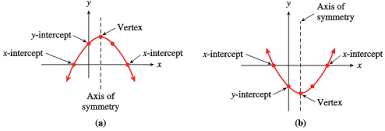
\includegraphics{parabola_graph.png}
}
\subsection{Parabolic Transformations}
\thm{Parabolic Transformations}{
    Parabola Transformations:
    \newline 
    if $a < 0$, the parabola is concave down
    \newline
    if $a > 0$, the parabola is concave up
    \newline
    if $c < 0$  move parabola down y axis
    \newline
    if $c > 0$  move parabola up y axis
    \newline
    if $b < 0$  move parabola left along x axis
    \newline
    if $b > 0$, the move parabola right along the x-axis
}
\section{Functions and their notation}
\thm{Functions and their notation}{
Functions are another way of writing equations for graphs, $y = x^{2}$ can be written as $f(x) = x^{2}$
\newline
Any set of ordered pairs is called a relation when referring to a function, a relation where each x value produces only one y value is called a function.
\newline
Any relation that also passes the vertical line test can be referred to as a Function.
\newline
The set of permissible x values in a relation is referred to as the domain
\newline
The range is the set of y coordinates the function can output into a relation
\begin{center}
    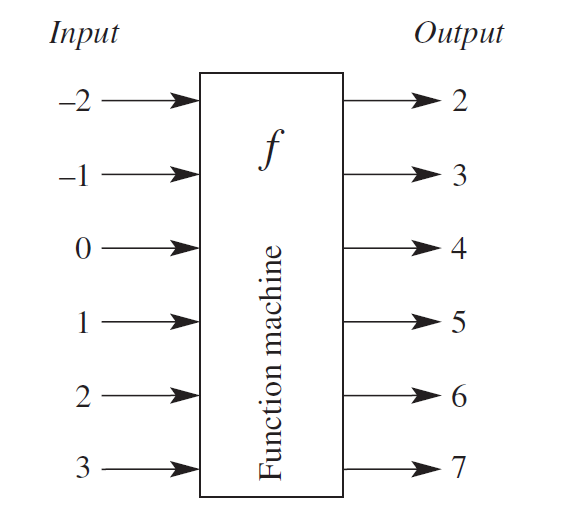
\includegraphics[scale=0.5]{functiongraphic.png}
\end{center}
}
\qs{}{\begin{center}$f(x) = 3x + 4$ find $f(\frac{1}{2})$ \end{center}}
$$f(\frac{1}{2}) = 3(\frac{1}{2}) + 4$$
$$= \frac{3}{2} + 4$$
$$= \frac{11}{2}$$
\qs{}{\begin{center} Find the domain of the following equation $f(x) = \frac{2}{x}$ \end{center}}
\begin{center}
    The domain for the equation is $x \neq 0$
\end{center}
\newpage
\section{Linear Relationships}
\subsection{Straight lines}
\subsubsection{Straight line formula}
\thm{Straight line formula}{
    Gradient states the slope of a line abbreviated to m in equations
    To find the gradient the equation is $\frac{y2-y1}{x2-x1}$
    \newline
    If the gradient is positive, the  slope is uphill
    If the gradient is negative, the slope is downhill
    No gradient = horizontal line
    Vertical line = Undefined line
\newline
    The straight line equation is $y = mx + c$
 where  m  is the  gradient and c  is the y-intercept
\newline


 
}
\raggedright
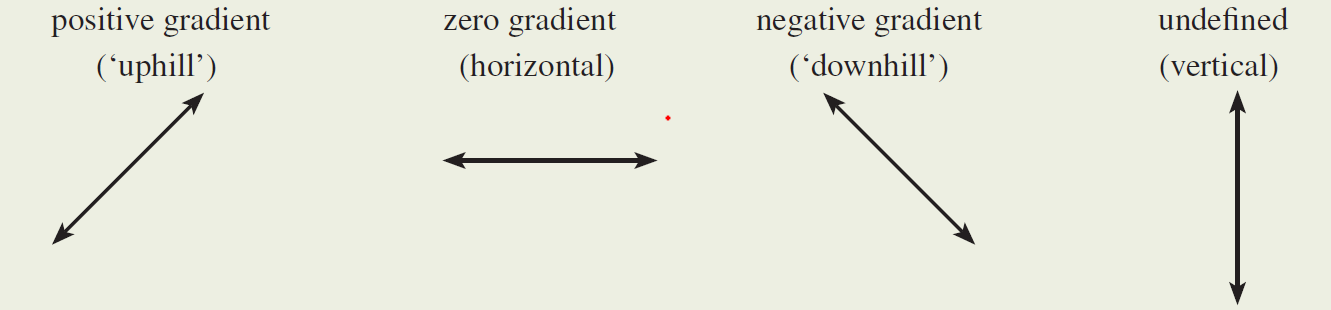
\includegraphics[scale=0.5]{gradient_lines.png}
\qs{Find Y intercept}{$$y = 2x - 8$$}
$$y = 2 \times 0 -8$$
$$ y = -8$$
\newline
\qs{Find equation of the line using the points below}{$$(3,11) (6,7)$$}
$$\frac{11-7}{3-6}$$
$$-\frac{4}{3}$$
$$y = -\frac{4}{3}x + c$$
$$11 = -\frac{4}{3} \times 3 + c$$
$$11 = 4 + c $$
$$c = 7$$
\newpage
\subsubsection{Point Gradient Formula}
\thm{Point Gradient Formula}{
    If you are given one point and  gradient, you can use $y-y1 = m(x-x1)$
    where (y1, x1,) are the points on the line and m is the gradient

}
\qs{Find the equation of the line }{$$(3,2) and m = 4$$}
$$y-2 = 4(x-3)$$
$$y-2 = 4x-12$$
$$y = 4x -10$$
\qs{Find the equation of the line}{$$(-3,-4) m = -1$$}
$$y + 4 = -1(x+3)$$
$$y + 4 = -x - 3$$
$$y = -x -7$$
\subsubsection{Additional formulas} 
\thm{Additional formulas}{
    Midpoint Formula:
    \newline
    The midpoint is  between two points of a line segment; the formula is
    $M= (\frac{x1+x2}{2},\frac{y1+y2}{2})$
    \newline
    Line Segment Length:
    \newline
    The length of a line segment is the distance between two points; the formula is 
    $d = \sqrt{(x2-x1)^{2}+ (y2 - y1)^{2}}$
}
\qs{Find the midpoint}{$$(-3,-5) and (2,8)$$}
$$M = (\frac{-3 + 2}{2}, \frac{8-5}{2})$$
$$ M =(-\frac{1}{2},\frac{3}{2})$$

\qs{Find the distance between the points}{$$(-3,8) and (4, -1)$$}
$$d = \sqrt{(4+3)^{2}+(-1-8)^{2}}$$
$$d = \sqrt{7^{2}+ 9^{2}}$$
$$d = \sqrt{130}$$
\subsubsection{Parallel and perpendicular lines}
\thm{Parallel and Perpendicular lines}{
    Parallel Lines:
    \newline
    All parallel lines have the same gradient
    \newline
    Perpendicular lines:
    \newline
    To find perpendicular lines $ m1 \times m2 = -1$ or $ m2 = -\frac{1}{m1}$, m2 is the negative reciprocal of m1

}
\qs{Are these lines perpendicular or parallel}{$$ y = \frac{1}{2}x + 2$$ \centering and $$ 2y - x = 5$$}
$$2y = x + 5$$
$$ y = \frac{1}{2}x + \frac{5}{2}$$
$$These lines are parallel to each other$$
\qs{Are these lines perpendicular or parallel}{$$ y = -3x-8$$ \centering and $$y = \frac{1}{3}x+ 1$$}
$$ -3 \times \frac{1}{3} = -1$$
$$Thes lines are perpendicular$$
\newpage
\subsection{Simultaneous Equations}
\subsubsection{Simultaneous Equations Substitution}
\thm{Simultaneous Equations Substitution}{
    The substitution method is used to solve simultaneous equations when one pronumeral is isolated and can be substituted into the other equation.
}
\qs{}{$$1.2x-3y = -8$$ $$2.y = x + 3$$}
\centering Sub 2 into 1
$$2x -3(x + 3) = -8$$
$$2x -3x -9 = -8$$
$$x = -1$$
$$ y = -1 + 3$$
$$y = 2$$
$$(-1,2)$$
\begin{note}
 Always remember to isolate pronumerals before substituting
\end{note}
\qs{}{$$1.y = -3x + 2$$  $$2.y = 7x -8$$}
\centering Sub 1 into 2
$$ 7x - 8 = -3x + 2$$
$$10x = 10$$
$$ x =  1$$
$$y = 7 -8$$
$$ y = -1$$
$$(1,-1)$$
\newpage
\raggedright
\subsubsection{Simultaneous Equations Elimination}
\thm{Simultaneous Equations Elimination}{
    The elimination method is used when you cannot isolate one variable, and the equation is in the form of $ax + by = d$
    \newline
    The method used to complete the elimination method is multiplying both equations by a chosen factor and then adding or subtracting one of the equations from the other to eliminate a variable.
}
\qs{}{$$1.x + y = 6$$ \centering $$2.3x - y = 10$$}
\centering add 1 to 2
2a.$$4x = 16$$
$$x = 4$$
$$4 + y = 6$$
$$ y = 2$$
\begin{note}
    Once you find one variable, sub into an equation to find the other
\end{note}

\qs{}{$$1.3x + 2y = 6$$ \centering and $$2.5x + 3y = 11$$}
\centering 1. times 3
\centering 2. times 2
$$1a. 9x + 6y = 18$$
$$2a. 10x + 6y = 22$$
\centering 2a - 1a
$$ x = 4$$
$$12 + 2y = 6$$
$$ y = -3$$
\begin{note}
    When multiplying the equations by the chosen factor, remember that  one coefficient and variable in each equation should be the same
\end{note}
\newpage
\raggedright
\subsection{Linear Inequalities}
\thm{Linear inequalities }{
    We solve Linear inequalities the same way we solve linear equations, except we flip the sign if we multiply or divide by a negative.
    \newline
    When drawing linear inequalities, we use an open circle if the greater or less than signs are used. We use a closed circle if the greater/less than or equal symbols are used.
}
\qs{}{$$3x + 4 > 13$$}
$$3x > 9$$
$$ x > 3$$
\qs{}{$$4 -\frac{x}{3} \leq 6$$}
$$-\frac{x}{3} \leq 2$$
$$x \geq -6$$
\section{Indices and Surds}
\subsection{Surds}
\subsection{Surd Rules and Simplification }
\thm{Surds Rules and Simplification }{
    Surds are irrational numbers that don't have a terminating decimal; surds use $ \sqrt{}$ 
    \newline
    Surd Rules:
    \newline
    $\sqrt{x^{2}} = x$
    \newline
    $\sqrt{xy} = \sqrt{x} \times \sqrt{y}$
    \newline
    $\sqrt{\frac{x}{y}} = \frac{\sqrt{x}}{\sqrt{y}}$
    \newline 
    When a factor of a number is a perfect square, its called a square factor
    \newline 
    Simplifying Surds:
    \newline
    To simplify a surd, look for square factors of that number $\sqrt{50} = \sqrt{25 \times 2} = 5\sqrt{2}$
}
\qs{Simplify the following Surd}{$$\sqrt{32}$$}
$$ \sqrt{16 \times 2}$$
$$4\sqrt{2}$$
\qs{Simplify the following Surd}{$$\sqrt{\frac{75}{9}} $$}
$$\frac{\sqrt{25 \times 3}}{3}$$
$$\frac{5\sqrt{3}}{3}$$
\subsubsection{Adding and Subtracting Surds}
\thm{Adding and Subtracting Surds}{
    Like surds are multiples of the same surd, only like surds can be added or subtracted. 
    \newline
    Remember to simplify surds before adding or subtracting them.
}
\qs{}{$$2\sqrt{3}+ 4\sqrt{3}$$}
$$=6\sqrt{3}$$
\qs{}{$$5\sqrt{2} - \sqrt{8}$$}
$$=5\sqrt{2} - \sqrt{4 \times 2} $$
$$=5\sqrt{2} - 2\sqrt{ \times 2} $$
$$3\sqrt{2}$$

\subsubsection{Multiplying and Dividing Surds}
\thm{Multiplying and Dividing}{
    When multiply surds use $a\sqrt{x} \times b\sqrt{y} = ab\sqrt{xy}$
    \newline
    When dividing surds use $\frac{a\sqrt{x}}{b\sqrt{y}} = \frac{a}{b} \sqrt{\frac{x}{y}}$
    \newline 
    Also, remember to use the distributive law to expand brackets.
}
\qs{}{$$2\sqrt{3} \times 3\sqrt{15}$$}
$$6 \sqrt{45}$$
$$6 \sqrt{9 \times 5}$$
$$18 \sqrt{5}$$
\begin{note}
    Remember to times all square numbers by the number multiply the surd as seen above
\end{note}
\qs{}{$$\frac{12\sqrt{18}}{3 \sqrt{3}}$$}
$$\frac{12}{3}\sqrt{\frac{18}{3}}$$
$$4\sqrt{6}$$
\begin{note}
    Always separate the fraction before simplifying when dividing Surds
\end{note}
\subsubsection{Rationalising the Denominator}
\thm{Rationalising the denominator}{
    Rationalising the denominator involves multiplying the entire fraction 
    by the surd, denominator to rationalise it to a whole number
}
\qs{}{$$\frac{2\sqrt{6}}{5\sqrt{2}}$$}
$$\frac{2\sqrt{6}}{5\sqrt{2}} \times \frac{\sqrt{2}}{\sqrt{2}}$$
$$\frac{2\sqrt{12}}{10}$$
$$\frac{4\sqrt{3}}{10}$$
$$\frac{2\sqrt{3}}{5}$$
\qs{}{$$\frac{1-\sqrt{3}}{\sqrt{3}}$$}
$$\frac{1-\sqrt{3}}{\sqrt{3}} \times \frac{\sqrt{3}}{\sqrt{3}}$$
$$\frac{\sqrt{3}-3}{3}$$
\newpage

\subsection{Indices}
\subsubsection{Fractional Indices}
\thm{Fractional Indices}{
    $a^{\frac{1}{n}} = \sqrt[n]{a}$
    this is the nth root of a
    \newline
    $a^{\frac{m}{n}}  = (\sqrt[n]{a})^{m}$
}
\qs{Write in index form}{$$\sqrt[4]{x^{7}}$$}
$$=x^{\frac{7}{4}}$$
\qs{Write in surd form}{$$5^{\frac{2}{3}}$$}
$$= \sqrt[3]{5^{2}}$$
\subsubsection{Exponential Equations}
\thm{Exponential Equations}{
    An exponential equation looks like $a^{x} = b$. There is only one 
    solution to an exponential equation like the above. Many of these equations can be solved by using 
    the same base for each exponent.
}

\qs{}{$$25^{x}= 125$$}
$$(5^{2})^{x} = 5^{3}$$
$$2x = 3$$
$$x = \frac{3}{2}$$

\qs{}{$$3^{2x-1}= 27^{x}$$}
$$3^{2x-1}= 3^{3x}$$
$$2x-1= 3x$$
$$x = -1$$
\newpage
\section{Statistics}
\subsection{Types of Statistics and Data Displays}
\thm{Types of Statistics and Data Displays}{
    Types of Statistics:
    \newline
    There are two types of Statistics Categorical and Numerical. Within these types, there are subsections or statistics.
    \newline
    For Categorical Data, there are nominal and Ordinal data. Nominal data has no order, i.e. red, green, blue. Ordinal data can be ordered, i.e. low, medium, and high.
    \newline
    For Numerical, there are Discrete and Continuous data. Discrete data can only have a limited amount of values, i.e. the number of children in a family. Continuous Data can take any value of numbers in a range, i.e. time taken to run a race.
    \newline
    Types of Data sets:
    \newline
    There are three types of data sets, Symmetrical where the mean and median will be equal, 
    \newline
    Positively Skewed where the median will be less than the mean and
   \newline
    Negatively skewed where the median will be greater than the mean.
    See the Figures Above for a visual representation.


}
\begin{figure}
    \centering
    \begin{subfigure}[b]{0.3\textwidth}
        \centering
        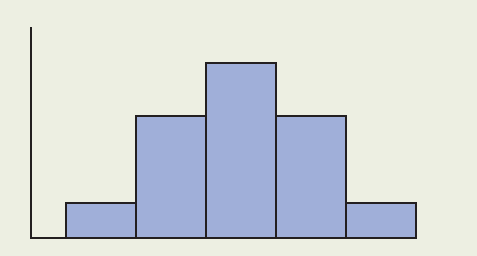
\includegraphics[width=\textwidth]{symmetrical_data.png}
        \caption{The median and mean will be equal}
        \label{Symmetrical Data}
    \end{subfigure}
    \hfill
    \begin{subfigure}[b]{0.3\textwidth}
        \centering
        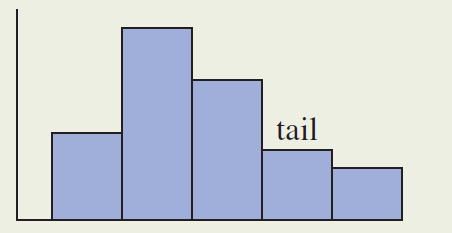
\includegraphics[width=\textwidth]{positive_data.png}
        \caption{The median will be less than the mean}
        \label{Positively skewed Data}
    \end{subfigure}
    \hfill
    \begin{subfigure}[b]{0.3\textwidth}
        \centering
        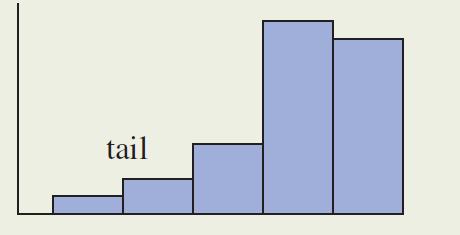
\includegraphics[width=\textwidth]{negative_data.png}
        \caption{The median will be greater than the mean}
        \label{Negatively Skewed Data}
    \end{subfigure}
       \caption{SYMMETRICAL AND SKEWED DATA}
       \label{fig: three graphs}
\end{figure}
\subsection{Summary Statistics}
\thm{Summary Statistics}{
    Summary statistics highlight important aspects of a data set
    \newline
    The median is the middle value of a data set. When the data set is even, you should divide the middle two numbers by 2
    \newline
    The mode is the most frequently occurring value in a dataset
    \newline
    \newline
    The frequency and the percentage frequency are the number of times a 
    favourable outcome occurred. To get percentage frequency, you 
    divide the number of favourable outcomes by the total outcomes.
    \newline
    \newline
    Five-figure summary:
    \newline
    Min/max value, the smallest/largest value in a dataset
    \newline
    Lower Quartile($Q_1$), the value above $25\%$ of the ordered data. The formula to obtain $Q_1$ is $ 0.25(n+1)$, with n being the number of data points given.
    \newline
    \newline
    The median($Q_2$), the value above $50\%$ of the ordered data.
    \newline
    \newline
    Upper Quartile($Q_3$), the value above $75\%$ of the ordered data. The formula to obtain $Q_1$ is $ 0.25(n+1)$, with n being the number of data points given.
    \newline
    \newline
    \newline
    A measure of spread:
    \newline
    Range = max value - min value
    \newline
    Interquartile Range(IQR). The formula for this is $Q_3 Q_1$
    \newline
    Standard deviation(SD)
    Outliers are outside the parameters o a data set. To detect if a data point is an outlier, the formula is  $ if <  Q_1 - 1.5 \times IQR $ or $ > Q_3 + 1.5 \times IQR$
}
\subsection{Box Plots}
\thm{Box Plots}{
    Box Plots are used to summarise data sets. The dataset is divided into four groups, as seen in the figure below,
    \begin{center}
        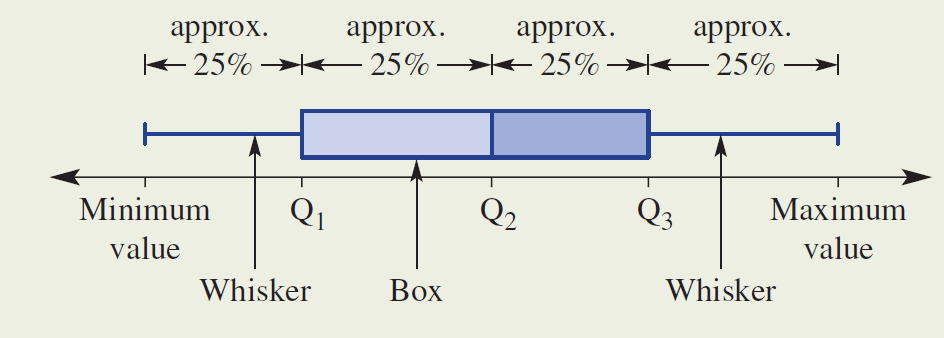
\includegraphics[scale=0.5]{boxplot.png} 
    \end{center}
    An outlier is marked with an x on the plot
}
\subsection{BiVariate Data}
\thm{Bivariate Data}{
    Types of correlation with bivariate data:
    \begin{center}
        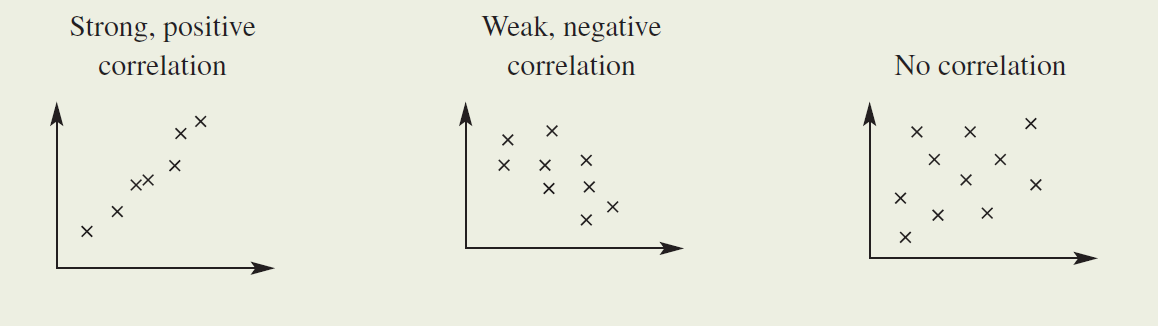
\includegraphics[scale=0.3]{correlation.png}
    \end{center}

}
\subsection{Line of Best fit}
\thm{Line of best fit}{
What is a line of best fit?
\newline
A line of best fit is placed on a graph with an even amount of points across each side. This shows the trend of the data.
\newline
To find the line of best fit, you can use the straight line formula or Point gradient Formula.
\newline
This line can be used for extrapolation or interpolation. 
}
\section{Probability}
\subsection{Arrays}
\thm{Arrays}{
An array is used to list the data of a two-step experiment.
If replacement is allowed in the experiment, then the outcome can occur in both steps of the experiment.
However, if replacement is not allowed, the outcome cannot occur in both steps of the experiment; w highlight these possibilities with an X in the array table.
}
\subsection{Tree Diagrams}
\thm{Tree Diagrams}{
Tree diagrams are used to list the probability of outcomes in an experiment with two or more steps
\newline
The branches on the tree describe the probability of an outcome at each stage. To gain the probability of an outcome occurring, you multiply the probability of each branch by each other.
See the diagram below for example:
}

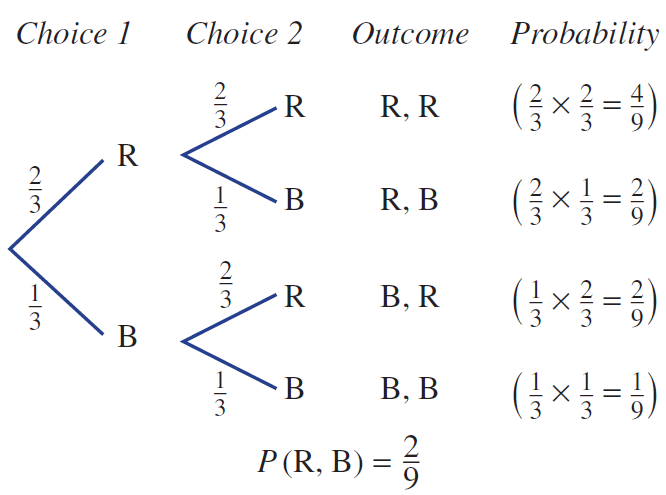
\includegraphics[scale=0.25]{treediagram.png}
\section{Measurement}
\subsection{Area of quadrilaterals }
\thm{Area of quadrilaterals}{
Area formulas:
\newline
Rhombus : $ \frac{1}{2}xy$
\newline
Parallelogram: $bh$
\newline 
Trapezium: $ h\left(\frac{a+b}{2}\right)$
\newline
Kite: $\frac{1}{2}xy$
}
\subsection{Cylinders and Prisms}
\subsubsection{SA  of Cylinders and Prisms}
\thm{SA of Cylinders and Prisms}{
    To find the Surface area of  objects, you need to find the area of each 2d shape that make up the 3d object
    \newline
    To find the SA of a cylinder, the formula is $2\pi$$r^{2}+ \pi$$dh$ with (d) being the diameter and (h) being the height
    \newline
    To find the SA of a prism, the formula is $ 2(w \times h) + 2(h \times l) + 2(l \times w)$
}
\qs{}{If the radius of a cylinder is three and the height of the cylinder is 3, what is the SA, leave your answer in exact form}
$$SA = 2\pi3^{2} + \pi6 \times 3$$

$$=18\pi + 18\pi$$
$$=36\pi$$
\qs{}{If the height of a prism is five and the length of the prism is seven, and the width of a prism is 2, find the SA}
$$SA = 2(2 \times 5) + 2(7 \times 5) + 2(2 \times 7) $$
$$= 40 + 70 + 28$$
$$=138$$
\newpage
\subsubsection{Volume of Cylinders and Prisms}
\thm{Volume of Cylinders and Prisms}{
To calculate the volume of a cylinder and prism, you first need to find the area of the cross-section that makes up that shape.
The volume formula for a cylinder is $ \pi$$r^{2} \times h$
\newline
The volume formula for a prism is $ah$, where a is the area of the cross-section of the shape.
}
\qs{}{Find the volume of a prism where the width is 2m, length is 3m, and height is 4 m}
$$V = 4(2 \times 3)$$
$$= 24$$

\qs{}{Find the volume of a cylinder where the radius is 2m and the height is 6m in exact form}
$$V = \pi2^{2} \times 6$$
$$ = 24\pi$$
\newpage
\subsection{Pyramids and cones}
\subsubsection{SA of Pyramids and Cones}
\thm{SA of Pyramids and Cones}{
    The formula for the surface area of a right cone is $\pi$$rl + \pi$$r^{2}$ where l is the slant height. If you need to find the slant height or any measurement in a  cone, use the Pythagorean theorem, the Sine rule or the Cosine Rule
    \newline
    The surface area for a right pyramid is $4(b \times h) + b^{2}$
}
\qs{}{The slant height of a cone is four and the radius of a cone is 6, what is the SA in exact form}
$$SA = \pi6 \times 7 + \pi6^{2}$$
$$= 42\pi + 36\pi$$
$$ = 78\pi$$
\qs{}{ The base of a pyramid is 4 and the height is 6 find the SA}
$$SA = 2(4 \times 6) + 4^{2}$$
$$= 48 + 16$$
$$= 64$$
\subsubsection{Volume of Pyramids and Cones}
\thm{Volume of Pyramids and Cones}{
To find the volume of a right pyramid or cone the formula $\frac{1}{3}AH$ where A is the area of the pyramids or cone cross-section, $x^{2}$ for pyramid  or$\pi$$r^{2}$ for cone.
 
}
\qs{}{Find the volume of this pyramid if the length is 4 and the height is 6}
$$V = \frac{1}{3}4^{2} \times 6$$
$$=\frac{16}{3} \times 6$$
$$=\frac{96}{3}$$
$$=32$$
\newpage
\qs{}{Find the volume of a cone in the exact form if the radius is 10 and the height is 15}
$$V =\frac{1}{3}(\pi10^{2}) \times 15$$
$$=\frac{100\pi}{3} \times 15$$
$$=\frac{1500\pi}{3}$$
$$=500\pi$$
\subsection{Spheres}
\subsubsection{SA of Spheres}
\thm{SA of Spheres}{
The formula for a Spheres SA is $4\pi$$r^{2}$
}
\qs{}{If the radius of the sphere is 3 find the SA in exact form}
$$SA = 4\pi3^{2}$$
$$=4\pi9$$
$$=36\pi$$
\qs{}{If the radius of a sphere is 5 find the SA in exact form}
$$SA=4\pi5^{2}$$
$$=100\pi$$
\subsubsection{Volume of a Sphere}
\thm{Volume of a Sphere}{
The formula for the Volume of a Sphere is $\frac{4}{3}\pi$$r^{3}$
}
\qs{}{If the Radius of the sphere is 7 find the volume in exact form}
$$\frac{4}{3}\pi7^{3}$$
$$\frac{4}{3}343\pi$$
$$\frac{1372\pi}{3}$$
\qs{}{If the radius of a sphere is 3 find the volume in exact form}
$$\frac{4}{3}\pi2^{3}$$
$$\frac{4}{3}8\pi$$
$$\frac{32\pi}{3}$$
\section{Trigonometry}
\subsection{Trigonometric Ratios}
\thm{Trigonometric Ratios}{
Trigonometric ratios help us find the angles inside a RAT
\newline
The three trigonometric Ratios:
\newline
$Sin\theta = \frac{opp}{hyp}$
\newline
$Cos\theta = \frac{adj}{hyp}$
\newline
$Tan\theta = \frac{opp}{adj}$
\newline
A mnemonic to remember these ratios is SOHCAHTOA
\newline
To find the unknown length of a side you can find a ratio that links the angle and the two sides together  and solve for $x$ See the second example below
\newline



}
\qs{}{Find the angle if the adjacent side is 5 and the hypotenuse 7 }
$$\cos\theta = \cos^{-1} \frac{5}{7}$$
$$\cos\theta = 44.4$$
\qs{}{Find the unknown side if the opp is 5cm, hyp = unknown and the angle is 50 }
$$\sin50 = \frac{5}{x}$$
$$x = \frac{5}{\sin50}$$
$$x = 6.53$$
\begin{note}
    Remember  if the variable is the numerator multiply the ratio and the length, if the variable is the denominator remember to divide the length by the variable
\end{note}
\subsection{Bearings}
\thm{Bearings \textbf{Come back to this later}}{
Bearings are three-digit numbers that give us a more accurate direction
}
\qs{}{}
\qs{}{}
\subsection{Obtuse Angles and Unit Circle}
\thm{Obtuse angles and Unit Circle}{
The unit circle has a radius of 1. It is used to define the values of $Cos\theta$ $Sin\theta$ and $Tan\theta$
\newline
Obtuse Angles:
\newline
To find the angle supplementary to an obtuse angle in the Q2 use the below 
\newline
$cos(180 - \theta)=  -cos\theta$
\newline
$sin(180 - \theta)= sin\theta$
\newline
$tan(180 - \theta)= -tan\theta$
\newline
A mnemonic to remember the sign in each of the four Quadrants is All Stations To Central(ALL SIN TAN COS) in the first quadrant(acute) all values are positive and in the Second only Sin is positive. etc.
\newline
\newline
Exact Values for the trigonometric Ratios can be obtained using two triangles seen below
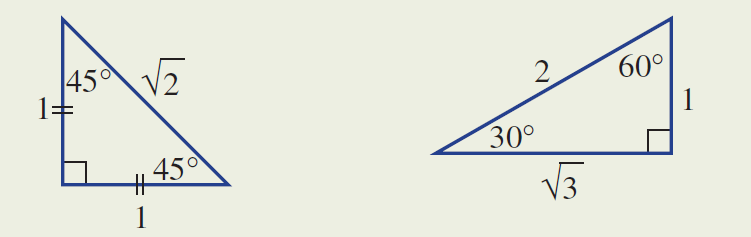
\includegraphics[scale=0.5]{exactvaluetriangles.png}
\newline
Here are the values in a table:
\begin{center}
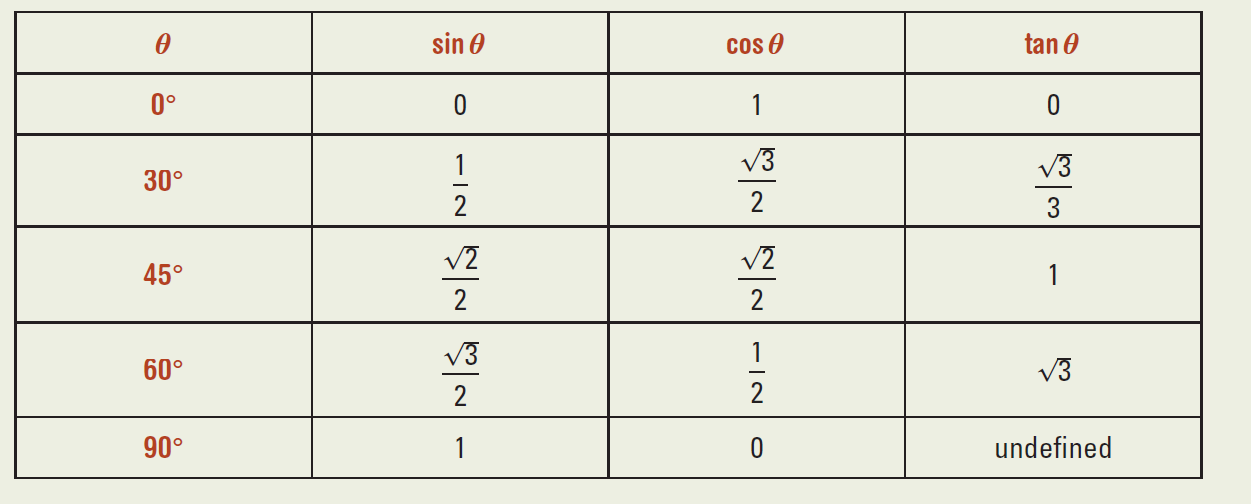
\includegraphics[scale=0.5]{exactvalues.png}
\end{center}
}
\newpage
\qs{}{Find the supplementary angle that goes with $\sin150$}
$$\theta=\sin180-150$$
$$=30$$
$$\sin30=\frac{1}{2}$$
\qs{}{Find the supplementary angle that goes with $\tan135$}
$$\theta=\tan180-135$$
$$= \tan45$$
$$\tan45 = 1$$

\subsection{Sine Rule}
\thm{The Sine Rule}{
 The Sine rule describes the relationship between the angles in a triangle and their opposite sides, being that they're equal.
 \newline
 the Sine Rule is $\frac{a}{\sin(A)} = \frac{b}{\sin(B)} = \frac{c}{\sin(C)}$, this rule can be manipulated to find either the side length or angle size.
 \newline
 It is important to note that to use the sine rule you need to know the size of one angle, the length of the side opposite that angle, and another side or angle.
\begin{center}
    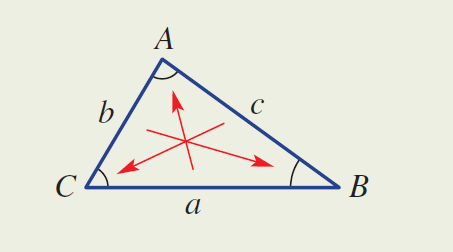
\includegraphics[scale=0.5]{sinediagram.png}   
\end{center}
}
\newpage
\qs{}{Find for x in the following: \begin{center}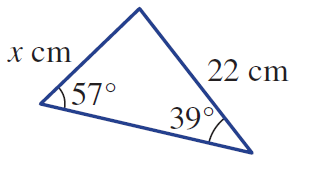
\includegraphics[scale=0.5]{qs1.png}\end{center}}
$$\frac{x}{\sin39}= \frac{22}{\sin57}$$
$$x = \frac{22 \times \sin39}{\sin57}$$
$$x = 16.51cm$$
\qs{}{Find $\theta$ in the following: \begin{center} 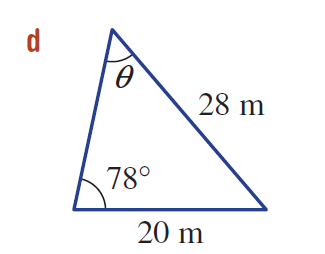
\includegraphics[scale=0.5]{qs2.png} \end{center}}
$$\frac{\sin\theta}{20}= \frac{\sin78}{28}$$
$$\sin\theta = \frac{20 \times \sin78}{28}$$
$$\sin\theta = 44.32$$
\begin{note}
    Remember to use $\sin^{-1}($ to gain the size of the angle. Additionally when using the sine rule to find  an angle, use the reciprocal of the rule stated in the theorem 
\end{note}
\newpage
\subsection{Cosine Rule}
\thm{Cosine Rule}{
    The cosine rule describes the relationship between three sides and one angle in a triangle.
    \newline
    The rule to find a side is $a^{2} = b^{2} + c^{2} - 2bc\times \cos(A)$
    \newline
    The rule to find the angle is $\cos(A) = \frac{b^{2} + c^{2} - a^{2}}{2bc}$
    \newline
    You can use the Cosine Rule when you are given two sides and angles and you are required to find the third side. You are required to find the angle when given three sides
    \newline
    Checking your answer, the longest side is opposite the largest $\angle  \therefore$ smallest angle is opp smallest $\angle$
}
\qs{}{Solve for the missing side \begin{center} 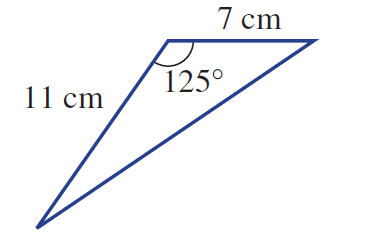
\includegraphics[scale=0.5]{qs3.png}\end{center}}
$$a^{2} = 7^{2} + 11^{2} -2\times 7 \times 11 \times \cos(125) $$
$$a = \sqrt{258.33}$$
$$a = 16.07cm$$
\qs{}{Solve for $\theta$ \begin{center} 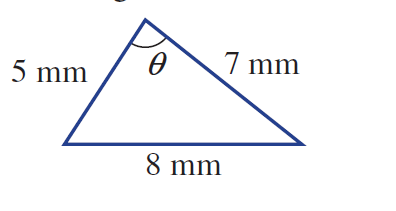
\includegraphics[scale=0.5]{qs4.png}\end{center}}
$$\cos\theta = \frac{5^{2}+7^{2}- 8^{2}}{2 \times 5 \times 7}$$
$$= \frac{10}{70}$$
$$= \cos^{-1}\left(\frac{1}{7}\right)$$
$$\theta=81.79$$
\newpage
\subsection{Area Rule}
\thm{Area Rule}{
The area rule is primarily used for NRATS but you can use it for RATS as well, it relates two sides of a triangle plus the including angle with the area.
\newline
The formula is $A = \frac{1}{2}ab\sin(C)$
}
\qs{}{Find the area \begin{center} 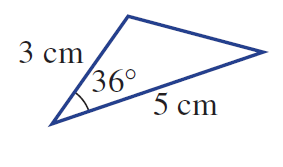
\includegraphics[scale=0.5]{qs5.png}\end{center}}
$$A = \frac{1}{2}\times 3 \times 5 \times \sin(36)$$
$$A= 4.41cm^{2}$$
\qs{}{Solve for x \begin{center} 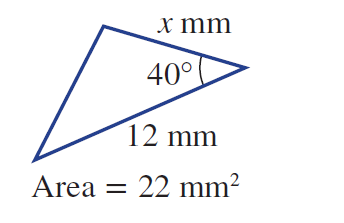
\includegraphics[scale=0.5]{qs6.png}\end{center}}
$$22 = \frac{1}{2}\times 12 \times x \times \sin(40) $$
$$\frac{22}{6\sin(40)} = x$$
$$x = 5.7mm^{2}$$
\newpage
\subsection{The four Quadrants}
\thm{The four Quadrants}{
   Dependent on the quadrant the angle is, the angle ratio could be positive or negative:
   \newline
   Q1(0-90): All ratios are positive
   \newline
   Q2(90-180): Only Sine Ratio is positive
    $180 - \theta$
    \newline
   Q3(180-270): Only the Tan ratio is positive, to get this angle the equation is $\theta - 180$
   \newline
   Q4(270-360): Only the Cosine ratio is positive the equation to find the cute angle is $360 - \theta$
   \newline
   A mnemonic to remember this is All Stations to Central
}
\qs{}{Find the acute angle if it is 280}

$$\theta = 360 - 280$$
$$\theta = 80 = -tan(80), -sin(80), cos(80)$$
\
\subsection{Trigonometric Function Graphs}
\thm{Trigonometric exact value graphs}{
    Here are the graphs that show the pattern of trigonometric exact values
    \newline
    Sine Wave:
    \begin{center}
    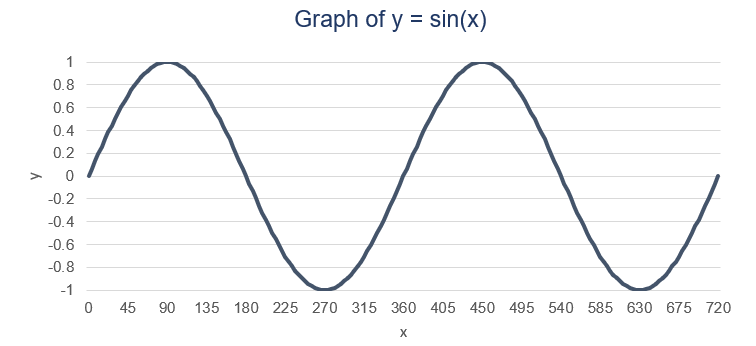
\includegraphics[scale=0.5]{sinewave.png}
    \newline
    \end{center}
    Cosine Wave:
    \begin{center}
    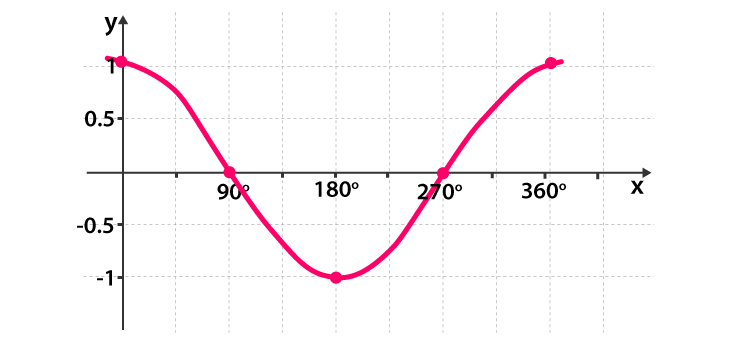
\includegraphics[scale=0.3]{coswave.png}
    \newline
    \end{center}
    Tangent Wave:
    \begin{center}
    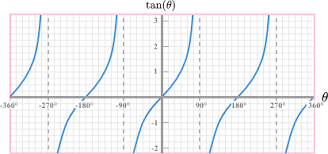
\includegraphics[scale=0.7]{tanwave.png}
    \end{center}

}
\section{Geometry}
\subsection{Triangle Congruency}
\thm{Triangle Congruency}{
Two triangles are considered to be congruent when they are the same shape and size

Triangle congruency can be proven using one of the tests below:
\newline
\newline 
SSS(3 Sides): The three sides of each triangle are equal to each other
\newline
SAS(Two sides one angle):  The two sides and the including angle of the triangles are equal to each other
\newline
AAS( Two angles and one side ): The two angles and one side of the triangles are equal
\newline
RHS(right-angle, hypotenuse, side): One side, 90-degree angle and the hypotenuse of triangles are equal 
}
\qs{}{Prove this pair of triangles is congruent \begin{center} 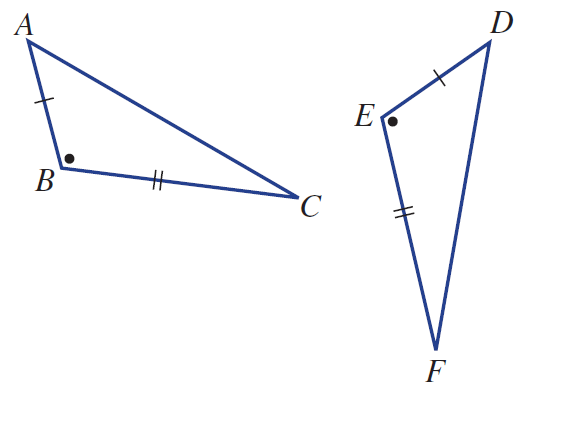
\includegraphics[scale=0.5]{qs7.png} \end{center}}
$$BC = EF (given)$$
$$AB = DE (given)$$
$$\angle ABC = \angle DEF (given)$$
$$\therefore \triangle ABC = \triangle DEF (SAS)$$
\qs{}{Prove this pair of triangles is congruent \begin{center} 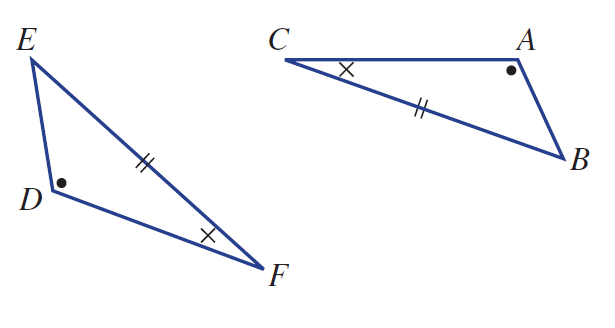
\includegraphics[scale=0.5]{QS8.png} \end{center}}
$$EF = CB (given)$$
$$\angle EDF = \angle CAB (given)$$
$$\angle EFD = \angle ACB (given)$$
$$\therefore \triangle EDF = \triangle CAB (AAS)$$
\newpage 
\subsection{Similarity in Shapes}

\thm{Similarity in Shapes}{
For two figures to be considered similar, they need to be the same shape(proportional) but have different 
sizes.
\newline
The symbol used to describe similarity in shapes is
\newline
To prove two shapes are similar we can use four different tests:
\newline
PPP(three proportional sides): Three sides of each triangle are proportional to each other
\newline
PAP(two proportional sides and included angle): Two sides of each triangle are proportional and the included angle is equal
\newline
AA(Two Angles): Two angles in each triangle are equal to each other
\newline
RHS(right angle, hypotenuse, side): The right angle, hypotenuse and side are proportional to each triangle

}
\qs{}{Prove these two triangles are similiar \begin{center} 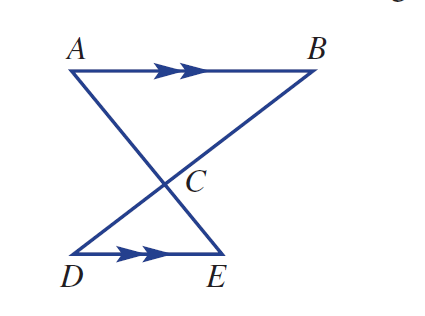
\includegraphics[scale=0.5]{qs9.png} \end{center}}
$$\angle DCE = \angle ACB (vert opp)$$
$$\angle CDE = \angle ABC (alt angles)$$
$$\therefore \triangle DCE ||| \triangle ACB (AA)$$

\qs{}{Prove these two triangles are similar \begin{center} \includegraphics[scale=0.5]{qs10.png} \end{center}}
$$\angle BAC  = \angle EDF (given)$$
$$\angle ABC  = \angle DEF $$
$$\therefore \triangle BAC ||| \triangle EDF (AA)$$
\subsection{Circle terminology and chord properties}
\begin{figure}
    \centering
    \begin{subfigure}[b]{0.3\textwidth}
        \centering
        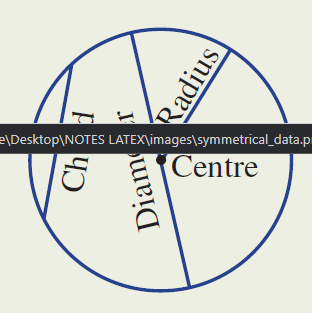
\includegraphics[width=\textwidth]{chord.png}
        \caption{The Chord is a segment whose both points lie on a circular arc}
        \label{Chord}
    \end{subfigure}
    \hfill
    \begin{subfigure}[b]{0.3\textwidth}
        \centering
        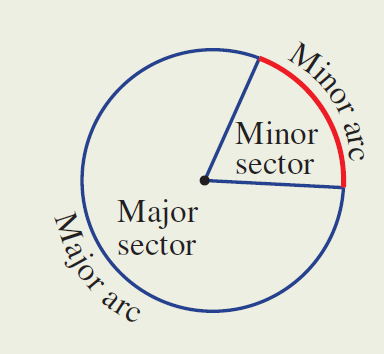
\includegraphics[width=\textwidth]{arc.png}
        \caption{An arc is a smooth curve joining two endpoints}
        \label{ARC}
    \end{subfigure}
    \hfill
    \begin{subfigure}[b]{0.3\textwidth}
        \centering
        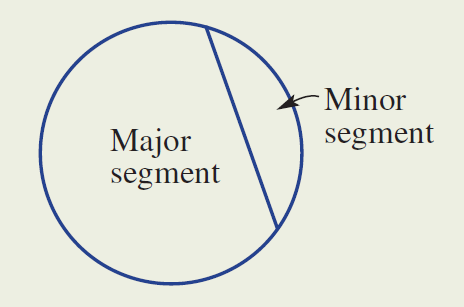
\includegraphics[width=\textwidth]{segment.png}
        \caption{A segment is part of the circle which is cut off by a chord or secant}
        \label{Segment}
    \end{subfigure}
       \caption{STypes of lines in Circles}
       \label{fig:three circles}
\end{figure}
\thm{Circle terminology and Chord properties}{
Look at the figures above to revise basic circle terms, an important term to remember is subtended which is a mathematical term for make/made.
\newline
An angle is subtended by an arc/chord when the arms of the angle arms meet the chord/arc's endpoint. See the example below.
\newline
\begin{center}
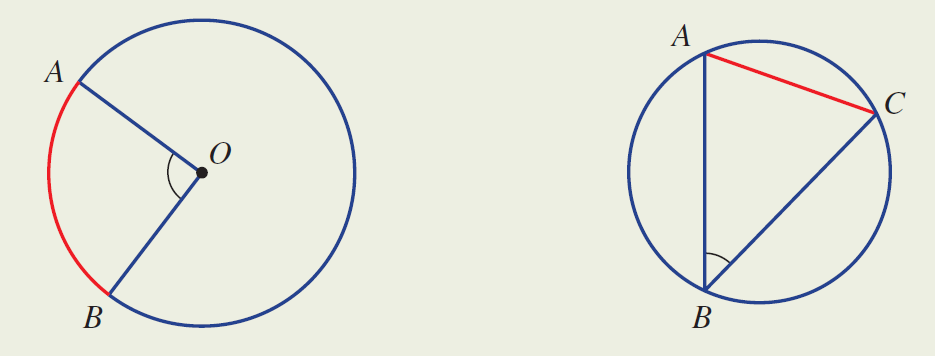
\includegraphics[scale=0.3]{chordangle.png}
\end{center}
Rules about Chords:
\newline
\noindent\begin{minipage}{0.3\textwidth}% adapt widths of mini pages to your needs
    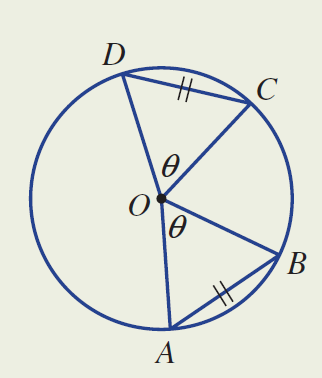
\includegraphics[width=\linewidth]{chordequal.png}
    \end{minipage}%
    \hfill%
    \begin{minipage}{0.6\textwidth}\raggedright
    Chords of equal length subtend equal angles at the centre of a circle, and chords that subtend equal angles are equal length.
    \end{minipage}

\noindent\begin{minipage}{0.3\textwidth}% adapt widths of minipages to your needs
    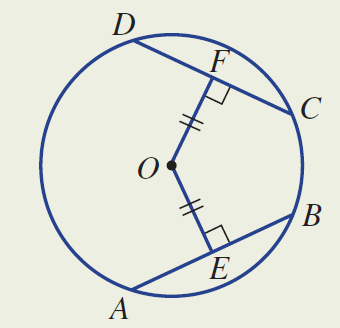
\includegraphics[width=\linewidth]{chordcentre.png}
\end{minipage}%
        \hfill%
\begin{minipage}{0.6\textwidth}\raggedright
        Chords which are equal distances from the centre are equal, and chords of equal length are equal distances from the centre.
\end{minipage}

\noindent\begin{minipage}{0.3\textwidth}% adapt widths of minipages to your needs
    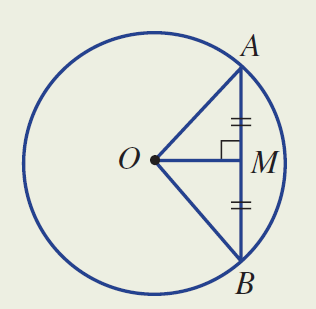
\includegraphics[width=\linewidth]{chordperp.png}
\end{minipage}%
        \hfill%
\begin{minipage}{0.6\textwidth}\raggedright
    The perpendicular from the centre of a circle bisects the chord, and a line through the centre of a circle that bisects a chord
    is perpendicular to the chord.
\end{minipage}
\noindent\begin{minipage}{0.3\textwidth}% adapt widths of mini pages to your needs
    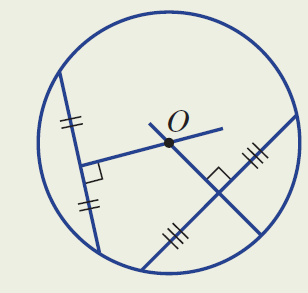
\includegraphics[width=\linewidth]{chordbisect.png}
\end{minipage}%
        \hfill%
\begin{minipage}{0.6\textwidth}\raggedright
Perpendicular bisectors of each chord intersect at the centre of a circle, you can use two perp bisectors to find the circle centre.
\end{minipage}

}


\qs{}{Given AB = CD and OE = 3 cm , find OF.\begin{center} 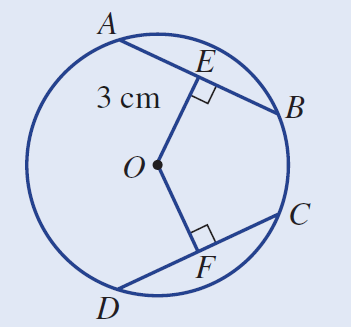
\includegraphics[scale=0.5]{qs11.png} \end{center}}
\ centre {$OF = 3cm$ (chords of equal length are the same distance from centre)}
\qs{}{Given $OM \perp AB$, AB = 10 cm and $\angle AOB = 92$ ,  find AM and $\angle AOM$ \begin{center} 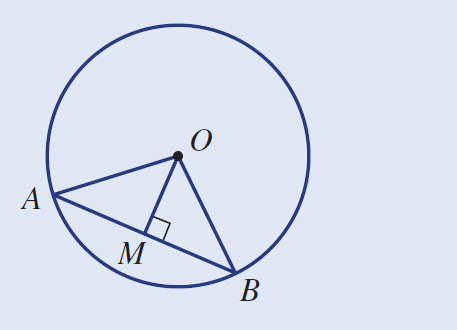
\includegraphics[scale=0.5]{qs12.png} \end{center}}
\center{$AM = 5cm$, perp centre bisects chord}
\begin{center}
    $\angle AOM = 92\div 2 = 46$
\end{center}
\raggedright
\subsection{Circle Angle properties}
\thm{Circle angle properties}{
     Here are the angle properties at the centre and circumference of a circle
     \newline
     The angle at the circumference of a circle is $\frac{1}{2}$ the size of the angle at the centre when standing on the same arc. The angle at the circumference is called an inscribed angle. See diagram.
     \begin{center}
        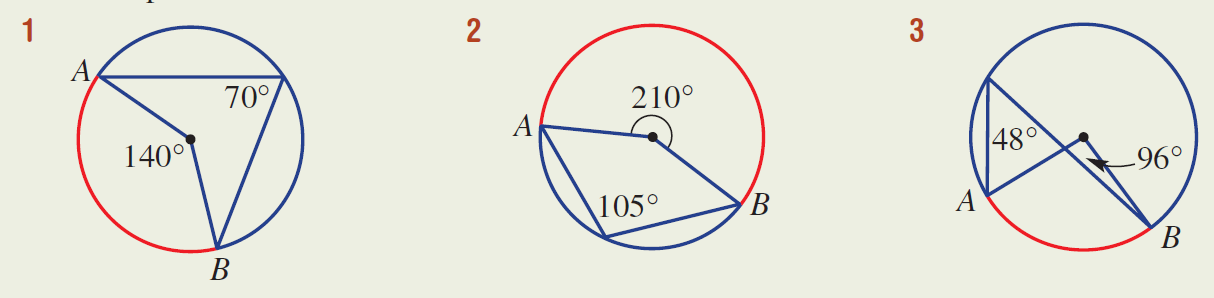
\includegraphics[scale=0.5]{circleangleprop.png}
     \end{center}
     The inscribed angle theory states that Angles subtended by the same arc are equal. See diagram.
     \begin{center}
        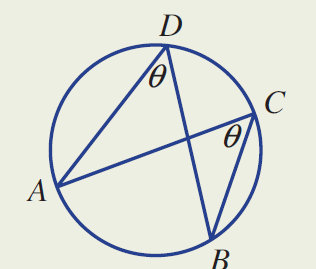
\includegraphics[scale=0.5]{inscribedangle.png}
     \end{center}
     The angle formed by the diameter to a point on a semi-circle is 90
     \begin{center}
        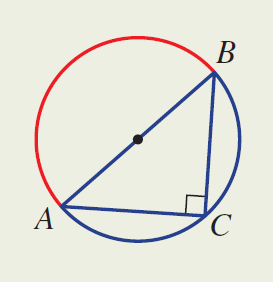
\includegraphics[scale=0.5]{diameterangle.png}
     \end{center}
     Opposite angles in a cyclic quadrilateral add to 180 degrees, as long as all vertices touch the circumference of the Circle. See diagram.
     \begin{center}
        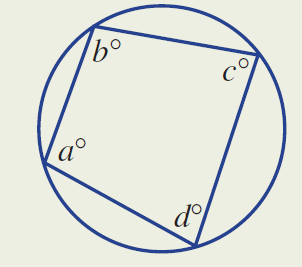
\includegraphics[scale=0.5]{cyclicquadangle.png}
     \end{center}
}
\qs{}{Find the value of $a$\begin{center}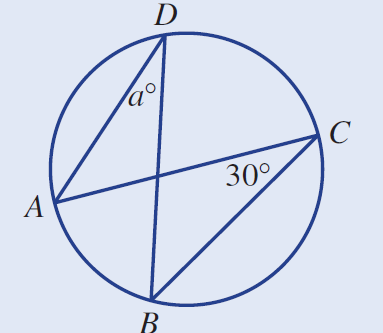
\includegraphics[scale=0.5]{QS13.png}\end{center}}
\begin{center}
    $a = 30$ inscribed angles on the same arc are equal
 \end{center}
 \qs{}{Find the value of $x$\begin{center}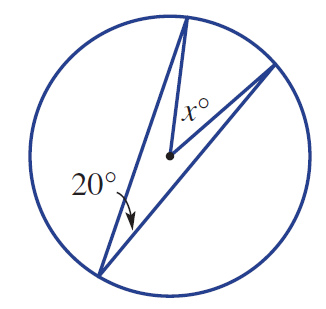
\includegraphics[scale=0.5]{qs14.png}\end{center}}
 \begin{center}
     $x = 80$ centre angles are 2 times the size of an inscribed angle when standing on the same arc
  \end{center}

\subsection{Tangent Theorems}
\thm{Tangent Theorems}{
    What is a tangent? A tangent is a line that has one point of contact with the circle/object.
    \newline
    In a circle, the tangent intersects the circle once and the tangent is perpendicular to the radius at the point of contact.
    \newline
    Two tangents that originate at the same point are equal.
    \newline
    Alternate angle theorem:
    \newline
    The angle formed between the tangent and the chord through the point of contact of the tangent is equal to the angle formed by the chord in the alternate segment. See diagram.
    \begin{center}
        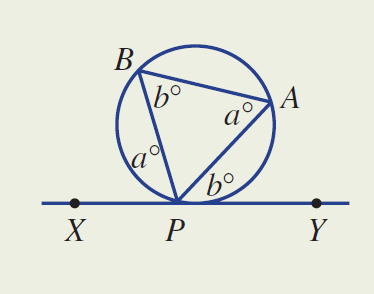
\includegraphics[scale=0.5]{alternateangletheorem.png}
     \end{center}
}
\qs{}{Solve for $a$     \begin{center}
    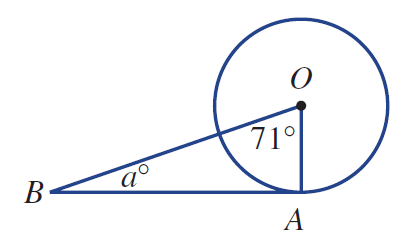
\includegraphics[scale=0.5]{qs15.png}
 \end{center}}
 \begin{center}
    $\angle BOA = 90$ alternate angle theorem
\end{center}
    $$180 -(90 + 71) = 19$$
    $$\therefore \angle OBA = 19$$
    \qs{}{Solve for $a$     \begin{center}
        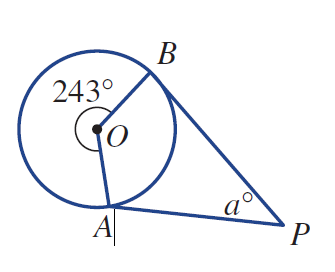
\includegraphics[scale=0.3]{qs16.png}
     \end{center}}
$$\angle BOA = 360-243 = 117$$
\begin{center}
$\angle OBP = \angle OAP = 90$ alternate angle theorem
\end{center}
$$a = 360- (117 + 90 + 90) = 63$$
$$a = 63$$
\section{Logarithms and Polynomials}
\subsection{Logarithm Intro}
\thm{Logarithm Intro}{
    Logarithms are is used to find the power a base was raised to get a value.
    \newline
    Example:
    \newline
    $\log_2(16)= 4$ since$   2^{4} = 16$
    \newline
    The way a log is written is the base is the subscript, and the value of the equation is inside the function which outputs the exponent ie $a^{x} = y$ $=\log_a(y) = x$
}
\qs{}{\centering Write $10^{2} = 100$ in log form}
$$\log_{10}(100) = 2$$
\qs{}{
\centering Write $\log_{7}(49) = 2$ in index form}
$$7^{2} = 49$$
\subsection{Log Laws}
\thm{Log Laws}{
    The Log laws Relate to index Laws, the log laws help us simplify and expand Logs  when needed
    \newline

    Product Rule:
    \newline
    $log_{a}(xy) = log_{a}(x) + log_{a}(y)$ This law relates to the  index law of $ a^{x}\times a^{y} = a^{x+y}$
    \newline
    Quotient Rule:
    \newline
    $\log_{a}(\frac{x}{y}) = \log_a{x} - log_{a}{y}$ This relates to $a^{m}\div a^{n} = a^{m-n}$
    \newline
    Power Rule:
    \newline
    $\log_{a}(x^{n}) = n\log_a{x}$ This law relates to $(a^{m})^{n}= a^{m\times n}$
    \newline
    Change of Base Rule:
    \newline
    $\log_{a}(x) = \frac{\log_{b}(x)}{\log_{b}(a)}$
    \newline
    $\log_a{\frac{1}{x}} = \log_{a}(x^{-1}) = -\log_{a}(x)$
}
\qs{}{Simplify$$\log_{a}(3)+ \log_{a}(2)$$}
$$\log_{a}(6)$$
\qs{}{Simplify$$2\log_{a}(3)$$}
$$\log_{a}(3^{2})$$
\end{document}\documentclass{report}

%%%%%%%%%%%%%%%%%%%%%%%%%%%%%%%%%
% PACKAGE IMPORTS
%%%%%%%%%%%%%%%%%%%%%%%%%%%%%%%%%


\usepackage[tmargin=2cm,rmargin=1in,lmargin=1in,margin=0.85in,bmargin=2cm,footskip=.2in]{geometry}
\usepackage{amsmath,amsfonts,amsthm,amssymb,mathtools}
\usepackage[varbb]{newpxmath}
\usepackage{xfrac}
\usepackage[makeroom]{cancel}
\usepackage{mathtools}
\usepackage{bookmark}
\usepackage{enumitem}
\usepackage{hyperref,theoremref}
\hypersetup{
	pdftitle={Assignment},
	colorlinks=true, linkcolor=doc!90,
	bookmarksnumbered=true,
	bookmarksopen=true
}
\usepackage[most,many,breakable]{tcolorbox}
\usepackage{xcolor}
\usepackage{varwidth}
\usepackage{varwidth}
\usepackage{etoolbox}
\usepackage{caption}
\usepackage{subcaption}
%\usepackage{authblk}
\usepackage{nameref}
\usepackage{multicol,array}
\usepackage{tikz-cd}
\usepackage[ruled,vlined,linesnumbered]{algorithm2e}
\usepackage{comment} % enables the use of multi-line comments (\ifx \fi) 
\usepackage{import}
\usepackage{xifthen}
\usepackage{pdfpages}
\usepackage{transparent}
\usepackage{graphicx}
\usepackage[utf8]{inputenc}
\newcommand\mycommfont[1]{\footnotesize\ttfamily\textcolor{blue}{#1}}
\SetCommentSty{mycommfont}
\newcommand{\incfig}[1]{%
    \def\svgwidth{\columnwidth}
    \import{./figures/}{#1.pdf_tex}
}

\usepackage{tikzsymbols}
\renewcommand\qedsymbol{$\Laughey$}


%\usepackage{import}
%\usepackage{xifthen}
%\usepackage{pdfpages}
%\usepackage{transparent}


%%%%%%%%%%%%%%%%%%%%%%%%%%%%%%
% SELF MADE COLORS
%%%%%%%%%%%%%%%%%%%%%%%%%%%%%%



\definecolor{myg}{RGB}{56, 140, 70}
\definecolor{myb}{RGB}{45, 111, 177}
\definecolor{myr}{RGB}{199, 68, 64}
\definecolor{mytheorembg}{HTML}{F2F2F9}
\definecolor{mytheoremfr}{HTML}{00007B}
\definecolor{mylenmabg}{HTML}{FFFAF8}
\definecolor{mylenmafr}{HTML}{983b0f}
\definecolor{mypropbg}{HTML}{f2fbfc}
\definecolor{mypropfr}{HTML}{191971}
\definecolor{myexamplebg}{HTML}{F2FBF8}
\definecolor{myexamplefr}{HTML}{88D6D1}
\definecolor{myexampleti}{HTML}{2A7F7F}
\definecolor{mydefinitbg}{HTML}{E5E5FF}
\definecolor{mydefinitfr}{HTML}{3F3FA3}
\definecolor{notesgreen}{RGB}{0,162,0}
\definecolor{myp}{RGB}{197, 92, 212}
\definecolor{mygr}{HTML}{2C3338}
\definecolor{myred}{RGB}{127,0,0}
\definecolor{myyellow}{RGB}{169,121,69}
\definecolor{myexercisebg}{HTML}{F2FBF8}
\definecolor{myexercisefg}{HTML}{88D6D1}


%%%%%%%%%%%%%%%%%%%%%%%%%%%%
% TCOLORBOX SETUPS
%%%%%%%%%%%%%%%%%%%%%%%%%%%%

\setlength{\parindent}{1cm}
%================================
% THEOREM BOX
%================================

\tcbuselibrary{theorems,skins,hooks}
\newtcbtheorem[number within=section]{Theorem}{Theorem}
{%
	enhanced,
	breakable,
	colback = mytheorembg,
	frame hidden,
	boxrule = 0sp,
	borderline west = {2pt}{0pt}{mytheoremfr},
	sharp corners,
	detach title,
	before upper = \tcbtitle\par\smallskip,
	coltitle = mytheoremfr,
	fonttitle = \bfseries\sffamily,
	description font = \mdseries,
	separator sign none,
	segmentation style={solid, mytheoremfr},
}
{th}

\tcbuselibrary{theorems,skins,hooks}
\newtcbtheorem[number within=chapter]{theorem}{Theorem}
{%
	enhanced,
	breakable,
	colback = mytheorembg,
	frame hidden,
	boxrule = 0sp,
	borderline west = {2pt}{0pt}{mytheoremfr},
	sharp corners,
	detach title,
	before upper = \tcbtitle\par\smallskip,
	coltitle = mytheoremfr,
	fonttitle = \bfseries\sffamily,
	description font = \mdseries,
	separator sign none,
	segmentation style={solid, mytheoremfr},
}
{th}


\tcbuselibrary{theorems,skins,hooks}
\newtcolorbox{Theoremcon}
{%
	enhanced
	,breakable
	,colback = mytheorembg
	,frame hidden
	,boxrule = 0sp
	,borderline west = {2pt}{0pt}{mytheoremfr}
	,sharp corners
	,description font = \mdseries
	,separator sign none
}

%================================
% Corollery
%================================
\tcbuselibrary{theorems,skins,hooks}
\newtcbtheorem[number within=section]{Corollary}{Corollary}
{%
	enhanced
	,breakable
	,colback = myp!10
	,frame hidden
	,boxrule = 0sp
	,borderline west = {2pt}{0pt}{myp!85!black}
	,sharp corners
	,detach title
	,before upper = \tcbtitle\par\smallskip
	,coltitle = myp!85!black
	,fonttitle = \bfseries\sffamily
	,description font = \mdseries
	,separator sign none
	,segmentation style={solid, myp!85!black}
}
{th}
\tcbuselibrary{theorems,skins,hooks}
\newtcbtheorem[number within=chapter]{corollary}{Corollary}
{%
	enhanced
	,breakable
	,colback = myp!10
	,frame hidden
	,boxrule = 0sp
	,borderline west = {2pt}{0pt}{myp!85!black}
	,sharp corners
	,detach title
	,before upper = \tcbtitle\par\smallskip
	,coltitle = myp!85!black
	,fonttitle = \bfseries\sffamily
	,description font = \mdseries
	,separator sign none
	,segmentation style={solid, myp!85!black}
}
{th}


%================================
% LENMA
%================================

\tcbuselibrary{theorems,skins,hooks}
\newtcbtheorem[number within=section]{Lenma}{Lenma}
{%
	enhanced,
	breakable,
	colback = mylenmabg,
	frame hidden,
	boxrule = 0sp,
	borderline west = {2pt}{0pt}{mylenmafr},
	sharp corners,
	detach title,
	before upper = \tcbtitle\par\smallskip,
	coltitle = mylenmafr,
	fonttitle = \bfseries\sffamily,
	description font = \mdseries,
	separator sign none,
	segmentation style={solid, mylenmafr},
}
{th}

\tcbuselibrary{theorems,skins,hooks}
\newtcbtheorem[number within=chapter]{lenma}{Lenma}
{%
	enhanced,
	breakable,
	colback = mylenmabg,
	frame hidden,
	boxrule = 0sp,
	borderline west = {2pt}{0pt}{mylenmafr},
	sharp corners,
	detach title,
	before upper = \tcbtitle\par\smallskip,
	coltitle = mylenmafr,
	fonttitle = \bfseries\sffamily,
	description font = \mdseries,
	separator sign none,
	segmentation style={solid, mylenmafr},
}
{th}


%================================
% PROPOSITION
%================================

\tcbuselibrary{theorems,skins,hooks}
\newtcbtheorem[number within=section]{Prop}{Proposition}
{%
	enhanced,
	breakable,
	colback = mypropbg,
	frame hidden,
	boxrule = 0sp,
	borderline west = {2pt}{0pt}{mypropfr},
	sharp corners,
	detach title,
	before upper = \tcbtitle\par\smallskip,
	coltitle = mypropfr,
	fonttitle = \bfseries\sffamily,
	description font = \mdseries,
	separator sign none,
	segmentation style={solid, mypropfr},
}
{th}

\tcbuselibrary{theorems,skins,hooks}
\newtcbtheorem[number within=chapter]{prop}{Proposition}
{%
	enhanced,
	breakable,
	colback = mypropbg,
	frame hidden,
	boxrule = 0sp,
	borderline west = {2pt}{0pt}{mypropfr},
	sharp corners,
	detach title,
	before upper = \tcbtitle\par\smallskip,
	coltitle = mypropfr,
	fonttitle = \bfseries\sffamily,
	description font = \mdseries,
	separator sign none,
	segmentation style={solid, mypropfr},
}
{th}


%================================
% CLAIM
%================================

\tcbuselibrary{theorems,skins,hooks}
\newtcbtheorem[number within=section]{claim}{Claim}
{%
	enhanced
	,breakable
	,colback = myg!10
	,frame hidden
	,boxrule = 0sp
	,borderline west = {2pt}{0pt}{myg}
	,sharp corners
	,detach title
	,before upper = \tcbtitle\par\smallskip
	,coltitle = myg!85!black
	,fonttitle = \bfseries\sffamily
	,description font = \mdseries
	,separator sign none
	,segmentation style={solid, myg!85!black}
}
{th}



%================================
% Exercise
%================================

\tcbuselibrary{theorems,skins,hooks}
\newtcbtheorem[number within=section]{Exercise}{Exercise}
{%
	enhanced,
	breakable,
	colback = myexercisebg,
	frame hidden,
	boxrule = 0sp,
	borderline west = {2pt}{0pt}{myexercisefg},
	sharp corners,
	detach title,
	before upper = \tcbtitle\par\smallskip,
	coltitle = myexercisefg,
	fonttitle = \bfseries\sffamily,
	description font = \mdseries,
	separator sign none,
	segmentation style={solid, myexercisefg},
}
{th}

\tcbuselibrary{theorems,skins,hooks}
\newtcbtheorem[number within=chapter]{exercise}{Exercise}
{%
	enhanced,
	breakable,
	colback = myexercisebg,
	frame hidden,
	boxrule = 0sp,
	borderline west = {2pt}{0pt}{myexercisefg},
	sharp corners,
	detach title,
	before upper = \tcbtitle\par\smallskip,
	coltitle = myexercisefg,
	fonttitle = \bfseries\sffamily,
	description font = \mdseries,
	separator sign none,
	segmentation style={solid, myexercisefg},
}
{th}

%================================
% EXAMPLE BOX
%================================

\newtcbtheorem[number within=section]{Example}{Example}
{%
	colback = myexamplebg
	,breakable
	,colframe = myexamplefr
	,coltitle = myexampleti
	,boxrule = 1pt
	,sharp corners
	,detach title
	,before upper=\tcbtitle\par\smallskip
	,fonttitle = \bfseries
	,description font = \mdseries
	,separator sign none
	,description delimiters parenthesis
}
{ex}

\newtcbtheorem[number within=chapter]{example}{Example}
{%
	colback = myexamplebg
	,breakable
	,colframe = myexamplefr
	,coltitle = myexampleti
	,boxrule = 1pt
	,sharp corners
	,detach title
	,before upper=\tcbtitle\par\smallskip
	,fonttitle = \bfseries
	,description font = \mdseries
	,separator sign none
	,description delimiters parenthesis
}
{ex}

%================================
% DEFINITION BOX
%================================

\newtcbtheorem[number within=section]{Definition}{Definition}{enhanced,
	before skip=2mm,after skip=2mm, colback=red!5,colframe=red!80!black,boxrule=0.5mm,
	attach boxed title to top left={xshift=1cm,yshift*=1mm-\tcboxedtitleheight}, varwidth boxed title*=-3cm,
	boxed title style={frame code={
					\path[fill=tcbcolback]
					([yshift=-1mm,xshift=-1mm]frame.north west)
					arc[start angle=0,end angle=180,radius=1mm]
					([yshift=-1mm,xshift=1mm]frame.north east)
					arc[start angle=180,end angle=0,radius=1mm];
					\path[left color=tcbcolback!60!black,right color=tcbcolback!60!black,
						middle color=tcbcolback!80!black]
					([xshift=-2mm]frame.north west) -- ([xshift=2mm]frame.north east)
					[rounded corners=1mm]-- ([xshift=1mm,yshift=-1mm]frame.north east)
					-- (frame.south east) -- (frame.south west)
					-- ([xshift=-1mm,yshift=-1mm]frame.north west)
					[sharp corners]-- cycle;
				},interior engine=empty,
		},
	fonttitle=\bfseries,
	title={#2},#1}{def}
\newtcbtheorem[number within=chapter]{definition}{Definition}{enhanced,
	before skip=2mm,after skip=2mm, colback=red!5,colframe=red!80!black,boxrule=0.5mm,
	attach boxed title to top left={xshift=1cm,yshift*=1mm-\tcboxedtitleheight}, varwidth boxed title*=-3cm,
	boxed title style={frame code={
					\path[fill=tcbcolback]
					([yshift=-1mm,xshift=-1mm]frame.north west)
					arc[start angle=0,end angle=180,radius=1mm]
					([yshift=-1mm,xshift=1mm]frame.north east)
					arc[start angle=180,end angle=0,radius=1mm];
					\path[left color=tcbcolback!60!black,right color=tcbcolback!60!black,
						middle color=tcbcolback!80!black]
					([xshift=-2mm]frame.north west) -- ([xshift=2mm]frame.north east)
					[rounded corners=1mm]-- ([xshift=1mm,yshift=-1mm]frame.north east)
					-- (frame.south east) -- (frame.south west)
					-- ([xshift=-1mm,yshift=-1mm]frame.north west)
					[sharp corners]-- cycle;
				},interior engine=empty,
		},
	fonttitle=\bfseries,
	title={#2},#1}{def}



%================================
% Solution BOX
%================================

\makeatletter
\newtcbtheorem{question}{Question}{enhanced,
	breakable,
	colback=white,
	colframe=myb!80!black,
	attach boxed title to top left={yshift*=-\tcboxedtitleheight},
	fonttitle=\bfseries,
	title={#2},
	boxed title size=title,
	boxed title style={%
			sharp corners,
			rounded corners=northwest,
			colback=tcbcolframe,
			boxrule=0pt,
		},
	underlay boxed title={%
			\path[fill=tcbcolframe] (title.south west)--(title.south east)
			to[out=0, in=180] ([xshift=5mm]title.east)--
			(title.center-|frame.east)
			[rounded corners=\kvtcb@arc] |-
			(frame.north) -| cycle;
		},
	#1
}{def}
\makeatother

%================================
% SOLUTION BOX
%================================

\makeatletter
\newtcolorbox{solution}{enhanced,
	breakable,
	colback=white,
	colframe=myg!80!black,
	attach boxed title to top left={yshift*=-\tcboxedtitleheight},
	title=Solution,
	boxed title size=title,
	boxed title style={%
			sharp corners,
			rounded corners=northwest,
			colback=tcbcolframe,
			boxrule=0pt,
		},
	underlay boxed title={%
			\path[fill=tcbcolframe] (title.south west)--(title.south east)
			to[out=0, in=180] ([xshift=5mm]title.east)--
			(title.center-|frame.east)
			[rounded corners=\kvtcb@arc] |-
			(frame.north) -| cycle;
		},
}
\makeatother

%================================
% Question BOX
%================================

\makeatletter
\newtcbtheorem{qstion}{Question}{enhanced,
	breakable,
	colback=white,
	colframe=mygr,
	attach boxed title to top left={yshift*=-\tcboxedtitleheight},
	fonttitle=\bfseries,
	title={#2},
	boxed title size=title,
	boxed title style={%
			sharp corners,
			rounded corners=northwest,
			colback=tcbcolframe,
			boxrule=0pt,
		},
	underlay boxed title={%
			\path[fill=tcbcolframe] (title.south west)--(title.south east)
			to[out=0, in=180] ([xshift=5mm]title.east)--
			(title.center-|frame.east)
			[rounded corners=\kvtcb@arc] |-
			(frame.north) -| cycle;
		},
	#1
}{def}
\makeatother

\newtcbtheorem[number within=chapter]{wconc}{Wrong Concept}{
	breakable,
	enhanced,
	colback=white,
	colframe=myr,
	arc=0pt,
	outer arc=0pt,
	fonttitle=\bfseries\sffamily\large,
	colbacktitle=myr,
	attach boxed title to top left={},
	boxed title style={
			enhanced,
			skin=enhancedfirst jigsaw,
			arc=3pt,
			bottom=0pt,
			interior style={fill=myr}
		},
	#1
}{def}



%================================
% NOTE BOX
%================================

\usetikzlibrary{arrows,calc,shadows.blur}
\tcbuselibrary{skins}
\newtcolorbox{note}[1][]{%
	enhanced jigsaw,
	colback=gray!20!white,%
	colframe=gray!80!black,
	size=small,
	boxrule=1pt,
	title=\textbf{Note:-},
	halign title=flush center,
	coltitle=black,
	breakable,
	drop shadow=black!50!white,
	attach boxed title to top left={xshift=1cm,yshift=-\tcboxedtitleheight/2,yshifttext=-\tcboxedtitleheight/2},
	minipage boxed title=1.5cm,
	boxed title style={%
			colback=white,
			size=fbox,
			boxrule=1pt,
			boxsep=2pt,
			underlay={%
					\coordinate (dotA) at ($(interior.west) + (-0.5pt,0)$);
					\coordinate (dotB) at ($(interior.east) + (0.5pt,0)$);
					\begin{scope}
						\clip (interior.north west) rectangle ([xshift=3ex]interior.east);
						\filldraw [white, blur shadow={shadow opacity=60, shadow yshift=-.75ex}, rounded corners=2pt] (interior.north west) rectangle (interior.south east);
					\end{scope}
					\begin{scope}[gray!80!black]
						\fill (dotA) circle (2pt);
						\fill (dotB) circle (2pt);
					\end{scope}
				},
		},
	#1,
}

%%%%%%%%%%%%%%%%%%%%%%%%%%%%%%
% SELF MADE COMMANDS
%%%%%%%%%%%%%%%%%%%%%%%%%%%%%%


\newcommand{\thm}[2]{\begin{Theorem}{#1}{}#2\end{Theorem}}
\newcommand{\cor}[2]{\begin{Corollary}{#1}{}#2\end{Corollary}}
\newcommand{\mlenma}[2]{\begin{Lenma}{#1}{}#2\end{Lenma}}
\newcommand{\mprop}[2]{\begin{Prop}{#1}{}#2\end{Prop}}
\newcommand{\clm}[3]{\begin{claim}{#1}{#2}#3\end{claim}}
\newcommand{\wc}[2]{\begin{wconc}{#1}{}\setlength{\parindent}{1cm}#2\end{wconc}}
\newcommand{\thmcon}[1]{\begin{Theoremcon}{#1}\end{Theoremcon}}
\newcommand{\ex}[2]{\begin{Example}{#1}{}#2\end{Example}}
\newcommand{\dfn}[2]{\begin{Definition}[colbacktitle=red!75!black]{#1}{}#2\end{Definition}}
\newcommand{\dfnc}[2]{\begin{definition}[colbacktitle=red!75!black]{#1}{}#2\end{definition}}
\newcommand{\qs}[2]{\begin{question}{#1}{}#2\end{question}}
\newcommand{\pf}[2]{\begin{myproof}[#1]#2\end{myproof}}
\newcommand{\nt}[1]{\begin{note}#1\end{note}}

\newcommand*\circled[1]{\tikz[baseline=(char.base)]{
		\node[shape=circle,draw,inner sep=1pt] (char) {#1};}}
\newcommand\getcurrentref[1]{%
	\ifnumequal{\value{#1}}{0}
	{??}
	{\the\value{#1}}%
}
\newcommand{\getCurrentSectionNumber}{\getcurrentref{section}}
\newenvironment{myproof}[1][\proofname]{%
	\proof[\bfseries #1: ]%
}{\endproof}

\newcommand{\mclm}[2]{\begin{myclaim}[#1]#2\end{myclaim}}
\newenvironment{myclaim}[1][\claimname]{\proof[\bfseries #1: ]}{}

\newcounter{mylabelcounter}

\makeatletter
\newcommand{\setword}[2]{%
	\phantomsection
	#1\def\@currentlabel{\unexpanded{#1}}\label{#2}%
}
\makeatother




\tikzset{
	symbol/.style={
			draw=none,
			every to/.append style={
					edge node={node [sloped, allow upside down, auto=false]{$#1$}}}
		}
}


% deliminators
\DeclarePairedDelimiter{\abs}{\lvert}{\rvert}
\DeclarePairedDelimiter{\norm}{\lVert}{\rVert}

\DeclarePairedDelimiter{\ceil}{\lceil}{\rceil}
\DeclarePairedDelimiter{\floor}{\lfloor}{\rfloor}
\DeclarePairedDelimiter{\round}{\lfloor}{\rceil}

\newsavebox\diffdbox
\newcommand{\slantedromand}{{\mathpalette\makesl{d}}}
\newcommand{\makesl}[2]{%
\begingroup
\sbox{\diffdbox}{$\mathsurround=0pt#1\mathrm{#2}$}%
\pdfsave
\pdfsetmatrix{1 0 0.2 1}%
\rlap{\usebox{\diffdbox}}%
\pdfrestore
\hskip\wd\diffdbox
\endgroup
}
\newcommand{\dd}[1][]{\ensuremath{\mathop{}\!\ifstrempty{#1}{%
\slantedromand\@ifnextchar^{\hspace{0.2ex}}{\hspace{0.1ex}}}%
{\slantedromand\hspace{0.2ex}^{#1}}}}
\ProvideDocumentCommand\dv{o m g}{%
  \ensuremath{%
    \IfValueTF{#3}{%
      \IfNoValueTF{#1}{%
        \frac{\dd #2}{\dd #3}%
      }{%
        \frac{\dd^{#1} #2}{\dd #3^{#1}}%
      }%
    }{%
      \IfNoValueTF{#1}{%
        \frac{\dd}{\dd #2}%
      }{%
        \frac{\dd^{#1}}{\dd #2^{#1}}%
      }%
    }%
  }%
}
\providecommand*{\pdv}[3][]{\frac{\partial^{#1}#2}{\partial#3^{#1}}}
%  - others
\DeclareMathOperator{\Lap}{\mathcal{L}}
\DeclareMathOperator{\Var}{Var} % varience
\DeclareMathOperator{\Cov}{Cov} % covarience
\DeclareMathOperator{\E}{E} % expected

% Since the amsthm package isn't loaded

% I prefer the slanted \leq
\let\oldleq\leq % save them in case they're every wanted
\let\oldgeq\geq
\renewcommand{\leq}{\leqslant}
\renewcommand{\geq}{\geqslant}

% % redefine matrix env to allow for alignment, use r as default
% \renewcommand*\env@matrix[1][r]{\hskip -\arraycolsep
%     \let\@ifnextchar\new@ifnextchar
%     \array{*\c@MaxMatrixCols #1}}


%\usepackage{framed}
%\usepackage{titletoc}
%\usepackage{etoolbox}
%\usepackage{lmodern}


%\patchcmd{\tableofcontents}{\contentsname}{\sffamily\contentsname}{}{}

%\renewenvironment{leftbar}
%{\def\FrameCommand{\hspace{6em}%
%		{\color{myyellow}\vrule width 2pt depth 6pt}\hspace{1em}}%
%	\MakeFramed{\parshape 1 0cm \dimexpr\textwidth-6em\relax\FrameRestore}\vskip2pt%
%}
%{\endMakeFramed}

%\titlecontents{chapter}
%[0em]{\vspace*{2\baselineskip}}
%{\parbox{4.5em}{%
%		\hfill\Huge\sffamily\bfseries\color{myred}\thecontentspage}%
%	\vspace*{-2.3\baselineskip}\leftbar\textsc{\small\chaptername~\thecontentslabel}\\\sffamily}
%{}{\endleftbar}
%\titlecontents{section}
%[8.4em]
%{\sffamily\contentslabel{3em}}{}{}
%{\hspace{0.5em}\nobreak\itshape\color{myred}\contentspage}
%\titlecontents{subsection}
%[8.4em]
%{\sffamily\contentslabel{3em}}{}{}  
%{\hspace{0.5em}\nobreak\itshape\color{myred}\contentspage}



%%%%%%%%%%%%%%%%%%%%%%%%%%%%%%%%%%%%%%%%%%%
% TABLE OF CONTENTS
%%%%%%%%%%%%%%%%%%%%%%%%%%%%%%%%%%%%%%%%%%%

\usepackage{tikz}
\definecolor{doc}{RGB}{0,60,110}
\usepackage{titletoc}
\contentsmargin{0cm}
\titlecontents{chapter}[3.7pc]
{\addvspace{30pt}%
	\begin{tikzpicture}[remember picture, overlay]%
		\draw[fill=doc!60,draw=doc!60] (-7,-.1) rectangle (-0.9,.5);%
		\pgftext[left,x=-3.5cm,y=0.2cm]{\color{white}\Large\sc\bfseries Chapter\ \thecontentslabel};%
	\end{tikzpicture}\color{doc!60}\large\sc\bfseries}%
{}
{}
{\;\titlerule\;\large\sc\bfseries Page \thecontentspage
	\begin{tikzpicture}[remember picture, overlay]
		\draw[fill=doc!60,draw=doc!60] (2pt,0) rectangle (4,0.1pt);
	\end{tikzpicture}}%
\titlecontents{section}[3.7pc]
{\addvspace{2pt}}
{\contentslabel[\thecontentslabel]{2pc}}
{}
{\hfill\small \thecontentspage}
[]
\titlecontents*{subsection}[3.7pc]
{\addvspace{-1pt}\small}
{}
{}
{\ --- \small\thecontentspage}
[ \textbullet\ ][]

\makeatletter
\renewcommand{\tableofcontents}{%
	\chapter*{%
	  \vspace*{-20\p@}%
	  \begin{tikzpicture}[remember picture, overlay]%
		  \pgftext[right,x=15cm,y=0.2cm]{\color{doc!60}\Huge\sc\bfseries \contentsname};%
		  \draw[fill=doc!60,draw=doc!60] (13,-.75) rectangle (20,1);%
		  \clip (13,-.75) rectangle (20,1);
		  \pgftext[right,x=15cm,y=0.2cm]{\color{white}\Huge\sc\bfseries \contentsname};%
	  \end{tikzpicture}}%
	\@starttoc{toc}}
\makeatother


%From M275 "Topology" at SJSU
\newcommand{\id}{\mathrm{id}}
\newcommand{\taking}[1]{\xrightarrow{#1}}
\newcommand{\inv}{^{-1}}

%From M170 "Introduction to Graph Theory" at SJSU
\DeclareMathOperator{\diam}{diam}
\DeclareMathOperator{\ord}{ord}
\newcommand{\defeq}{\overset{\mathrm{def}}{=}}

%From the USAMO .tex files
\newcommand{\ts}{\textsuperscript}
\newcommand{\dg}{^\circ}
\newcommand{\ii}{\item}

% % From Math 55 and Math 145 at Harvard
% \newenvironment{subproof}[1][Proof]{%
% \begin{proof}[#1] \renewcommand{\qedsymbol}{$\blacksquare$}}%
% {\end{proof}}

\newcommand{\liff}{\leftrightarrow}
\newcommand{\lthen}{\rightarrow}
\newcommand{\opname}{\operatorname}
\newcommand{\surjto}{\twoheadrightarrow}
\newcommand{\injto}{\hookrightarrow}
\newcommand{\On}{\mathrm{On}} % ordinals
\DeclareMathOperator{\img}{im} % Image
\DeclareMathOperator{\Img}{Im} % Image
\DeclareMathOperator{\coker}{coker} % Cokernel
\DeclareMathOperator{\Coker}{Coker} % Cokernel
\DeclareMathOperator{\Ker}{Ker} % Kernel
\DeclareMathOperator{\rank}{rank}
\DeclareMathOperator{\Spec}{Spec} % spectrum
\DeclareMathOperator{\Tr}{Tr} % trace
\DeclareMathOperator{\pr}{pr} % projection
\DeclareMathOperator{\ext}{ext} % extension
\DeclareMathOperator{\pred}{pred} % predecessor
\DeclareMathOperator{\dom}{dom} % domain
\DeclareMathOperator{\ran}{ran} % range
\DeclareMathOperator{\Hom}{Hom} % homomorphism
\DeclareMathOperator{\Mor}{Mor} % morphisms
\DeclareMathOperator{\End}{End} % endomorphism

\newcommand{\eps}{\epsilon}
\newcommand{\veps}{\varepsilon}
\newcommand{\ol}{\overline}
\newcommand{\ul}{\underline}
\newcommand{\wt}{\widetilde}
\newcommand{\wh}{\widehat}
\newcommand{\vocab}[1]{\textbf{\color{blue} #1}}
\providecommand{\half}{\frac{1}{2}}
\newcommand{\dang}{\measuredangle} %% Directed angle
\newcommand{\ray}[1]{\overrightarrow{#1}}
\newcommand{\seg}[1]{\overline{#1}}
\newcommand{\arc}[1]{\wideparen{#1}}
\DeclareMathOperator{\cis}{cis}
\DeclareMathOperator*{\lcm}{lcm}
\DeclareMathOperator*{\argmin}{arg min}
\DeclareMathOperator*{\argmax}{arg max}
\newcommand{\cycsum}{\sum_{\mathrm{cyc}}}
\newcommand{\symsum}{\sum_{\mathrm{sym}}}
\newcommand{\cycprod}{\prod_{\mathrm{cyc}}}
\newcommand{\symprod}{\prod_{\mathrm{sym}}}
\newcommand{\Qed}{\begin{flushright}\qed\end{flushright}}
\newcommand{\parinn}{\setlength{\parindent}{1cm}}
\newcommand{\parinf}{\setlength{\parindent}{0cm}}
% \newcommand{\norm}{\|\cdot\|}
\newcommand{\inorm}{\norm_{\infty}}
\newcommand{\opensets}{\{V_{\alpha}\}_{\alpha\in I}}
\newcommand{\oset}{V_{\alpha}}
\newcommand{\opset}[1]{V_{\alpha_{#1}}}
\newcommand{\lub}{\text{lub}}
\newcommand{\del}[2]{\frac{\partial #1}{\partial #2}}
\newcommand{\Del}[3]{\frac{\partial^{#1} #2}{\partial^{#1} #3}}
\newcommand{\deld}[2]{\dfrac{\partial #1}{\partial #2}}
\newcommand{\Deld}[3]{\dfrac{\partial^{#1} #2}{\partial^{#1} #3}}
\newcommand{\lm}{\lambda}
\newcommand{\uin}{\mathbin{\rotatebox[origin=c]{90}{$\in$}}}
\newcommand{\usubset}{\mathbin{\rotatebox[origin=c]{90}{$\subset$}}}
\newcommand{\lt}{\left}
\newcommand{\rt}{\right}
\newcommand{\bs}[1]{\boldsymbol{#1}}
\newcommand{\exs}{\exists}
\newcommand{\st}{\strut}
\newcommand{\dps}[1]{\displaystyle{#1}}

\newcommand{\sol}{\setlength{\parindent}{0cm}\textbf{\textit{Solution:}}\setlength{\parindent}{1cm} }
\newcommand{\solve}[1]{\setlength{\parindent}{0cm}\textbf{\textit{Solution: }}\setlength{\parindent}{1cm}#1 \Qed}

% Things Lie
\newcommand{\kb}{\mathfrak b}
\newcommand{\kg}{\mathfrak g}
\newcommand{\kh}{\mathfrak h}
\newcommand{\kn}{\mathfrak n}
\newcommand{\ku}{\mathfrak u}
\newcommand{\kz}{\mathfrak z}
\DeclareMathOperator{\Ext}{Ext} % Ext functor
\DeclareMathOperator{\Tor}{Tor} % Tor functor
\newcommand{\gl}{\opname{\mathfrak{gl}}} % frak gl group
\renewcommand{\sl}{\opname{\mathfrak{sl}}} % frak sl group chktex 6

% More script letters etc.
\newcommand{\SA}{\mathcal A}
\newcommand{\SB}{\mathcal B}
\newcommand{\SC}{\mathcal C}
\newcommand{\SF}{\mathcal F}
\newcommand{\SG}{\mathcal G}
\newcommand{\SH}{\mathcal H}
\newcommand{\OO}{\mathcal O}

\newcommand{\SCA}{\mathscr A}
\newcommand{\SCB}{\mathscr B}
\newcommand{\SCC}{\mathscr C}
\newcommand{\SCD}{\mathscr D}
\newcommand{\SCE}{\mathscr E}
\newcommand{\SCF}{\mathscr F}
\newcommand{\SCG}{\mathscr G}
\newcommand{\SCH}{\mathscr H}

% Mathfrak primes
\newcommand{\km}{\mathfrak m}
\newcommand{\kp}{\mathfrak p}
\newcommand{\kq}{\mathfrak q}

% number sets
\newcommand{\RR}[1][]{\ensuremath{\ifstrempty{#1}{\mathbb{R}}{\mathbb{R}^{#1}}}}
\newcommand{\NN}[1][]{\ensuremath{\ifstrempty{#1}{\mathbb{N}}{\mathbb{N}^{#1}}}}
\newcommand{\ZZ}[1][]{\ensuremath{\ifstrempty{#1}{\mathbb{Z}}{\mathbb{Z}^{#1}}}}
\newcommand{\QQ}[1][]{\ensuremath{\ifstrempty{#1}{\mathbb{Q}}{\mathbb{Q}^{#1}}}}
\newcommand{\CC}[1][]{\ensuremath{\ifstrempty{#1}{\mathbb{C}}{\mathbb{C}^{#1}}}}
\newcommand{\PP}[1][]{\ensuremath{\ifstrempty{#1}{\mathbb{P}}{\mathbb{P}^{#1}}}}
\newcommand{\HH}[1][]{\ensuremath{\ifstrempty{#1}{\mathbb{H}}{\mathbb{H}^{#1}}}}
\newcommand{\FF}[1][]{\ensuremath{\ifstrempty{#1}{\mathbb{F}}{\mathbb{F}^{#1}}}}
% expected value
\newcommand{\EE}{\ensuremath{\mathbb{E}}}
\newcommand{\charin}{\text{ char }}
\DeclareMathOperator{\sign}{sign}
\DeclareMathOperator{\Aut}{Aut}
\DeclareMathOperator{\Inn}{Inn}
\DeclareMathOperator{\Syl}{Syl}
\DeclareMathOperator{\Gal}{Gal}
\DeclareMathOperator{\GL}{GL} % General linear group
\DeclareMathOperator{\SL}{SL} % Special linear group

%---------------------------------------
% BlackBoard Math Fonts :-
%---------------------------------------

%Captital Letters
\newcommand{\bbA}{\mathbb{A}}	\newcommand{\bbB}{\mathbb{B}}
\newcommand{\bbC}{\mathbb{C}}	\newcommand{\bbD}{\mathbb{D}}
\newcommand{\bbE}{\mathbb{E}}	\newcommand{\bbF}{\mathbb{F}}
\newcommand{\bbG}{\mathbb{G}}	\newcommand{\bbH}{\mathbb{H}}
\newcommand{\bbI}{\mathbb{I}}	\newcommand{\bbJ}{\mathbb{J}}
\newcommand{\bbK}{\mathbb{K}}	\newcommand{\bbL}{\mathbb{L}}
\newcommand{\bbM}{\mathbb{M}}	\newcommand{\bbN}{\mathbb{N}}
\newcommand{\bbO}{\mathbb{O}}	\newcommand{\bbP}{\mathbb{P}}
\newcommand{\bbQ}{\mathbb{Q}}	\newcommand{\bbR}{\mathbb{R}}
\newcommand{\bbS}{\mathbb{S}}	\newcommand{\bbT}{\mathbb{T}}
\newcommand{\bbU}{\mathbb{U}}	\newcommand{\bbV}{\mathbb{V}}
\newcommand{\bbW}{\mathbb{W}}	\newcommand{\bbX}{\mathbb{X}}
\newcommand{\bbY}{\mathbb{Y}}	\newcommand{\bbZ}{\mathbb{Z}}

%---------------------------------------
% MathCal Fonts :-
%---------------------------------------

%Captital Letters
\newcommand{\mcA}{\mathcal{A}}	\newcommand{\mcB}{\mathcal{B}}
\newcommand{\mcC}{\mathcal{C}}	\newcommand{\mcD}{\mathcal{D}}
\newcommand{\mcE}{\mathcal{E}}	\newcommand{\mcF}{\mathcal{F}}
\newcommand{\mcG}{\mathcal{G}}	\newcommand{\mcH}{\mathcal{H}}
\newcommand{\mcI}{\mathcal{I}}	\newcommand{\mcJ}{\mathcal{J}}
\newcommand{\mcK}{\mathcal{K}}	\newcommand{\mcL}{\mathcal{L}}
\newcommand{\mcM}{\mathcal{M}}	\newcommand{\mcN}{\mathcal{N}}
\newcommand{\mcO}{\mathcal{O}}	\newcommand{\mcP}{\mathcal{P}}
\newcommand{\mcQ}{\mathcal{Q}}	\newcommand{\mcR}{\mathcal{R}}
\newcommand{\mcS}{\mathcal{S}}	\newcommand{\mcT}{\mathcal{T}}
\newcommand{\mcU}{\mathcal{U}}	\newcommand{\mcV}{\mathcal{V}}
\newcommand{\mcW}{\mathcal{W}}	\newcommand{\mcX}{\mathcal{X}}
\newcommand{\mcY}{\mathcal{Y}}	\newcommand{\mcZ}{\mathcal{Z}}


%---------------------------------------
% Bold Math Fonts :-
%---------------------------------------

%Captital Letters
\newcommand{\bmA}{\boldsymbol{A}}	\newcommand{\bmB}{\boldsymbol{B}}
\newcommand{\bmC}{\boldsymbol{C}}	\newcommand{\bmD}{\boldsymbol{D}}
\newcommand{\bmE}{\boldsymbol{E}}	\newcommand{\bmF}{\boldsymbol{F}}
\newcommand{\bmG}{\boldsymbol{G}}	\newcommand{\bmH}{\boldsymbol{H}}
\newcommand{\bmI}{\boldsymbol{I}}	\newcommand{\bmJ}{\boldsymbol{J}}
\newcommand{\bmK}{\boldsymbol{K}}	\newcommand{\bmL}{\boldsymbol{L}}
\newcommand{\bmM}{\boldsymbol{M}}	\newcommand{\bmN}{\boldsymbol{N}}
\newcommand{\bmO}{\boldsymbol{O}}	\newcommand{\bmP}{\boldsymbol{P}}
\newcommand{\bmQ}{\boldsymbol{Q}}	\newcommand{\bmR}{\boldsymbol{R}}
\newcommand{\bmS}{\boldsymbol{S}}	\newcommand{\bmT}{\boldsymbol{T}}
\newcommand{\bmU}{\boldsymbol{U}}	\newcommand{\bmV}{\boldsymbol{V}}
\newcommand{\bmW}{\boldsymbol{W}}	\newcommand{\bmX}{\boldsymbol{X}}
\newcommand{\bmY}{\boldsymbol{Y}}	\newcommand{\bmZ}{\boldsymbol{Z}}
%Small Letters
\newcommand{\bma}{\boldsymbol{a}}	\newcommand{\bmb}{\boldsymbol{b}}
\newcommand{\bmc}{\boldsymbol{c}}	\newcommand{\bmd}{\boldsymbol{d}}
\newcommand{\bme}{\boldsymbol{e}}	\newcommand{\bmf}{\boldsymbol{f}}
\newcommand{\bmg}{\boldsymbol{g}}	\newcommand{\bmh}{\boldsymbol{h}}
\newcommand{\bmi}{\boldsymbol{i}}	\newcommand{\bmj}{\boldsymbol{j}}
\newcommand{\bmk}{\boldsymbol{k}}	\newcommand{\bml}{\boldsymbol{l}}
\newcommand{\bmm}{\boldsymbol{m}}	\newcommand{\bmn}{\boldsymbol{n}}
\newcommand{\bmo}{\boldsymbol{o}}	\newcommand{\bmp}{\boldsymbol{p}}
\newcommand{\bmq}{\boldsymbol{q}}	\newcommand{\bmr}{\boldsymbol{r}}
\newcommand{\bms}{\boldsymbol{s}}	\newcommand{\bmt}{\boldsymbol{t}}
\newcommand{\bmu}{\boldsymbol{u}}	\newcommand{\bmv}{\boldsymbol{v}}
\newcommand{\bmw}{\boldsymbol{w}}	\newcommand{\bmx}{\boldsymbol{x}}
\newcommand{\bmy}{\boldsymbol{y}}	\newcommand{\bmz}{\boldsymbol{z}}

%---------------------------------------
% Scr Math Fonts :-
%---------------------------------------

\newcommand{\sA}{{\mathscr{A}}}   \newcommand{\sB}{{\mathscr{B}}}
\newcommand{\sC}{{\mathscr{C}}}   \newcommand{\sD}{{\mathscr{D}}}
\newcommand{\sE}{{\mathscr{E}}}   \newcommand{\sF}{{\mathscr{F}}}
\newcommand{\sG}{{\mathscr{G}}}   \newcommand{\sH}{{\mathscr{H}}}
\newcommand{\sI}{{\mathscr{I}}}   \newcommand{\sJ}{{\mathscr{J}}}
\newcommand{\sK}{{\mathscr{K}}}   \newcommand{\sL}{{\mathscr{L}}}
\newcommand{\sM}{{\mathscr{M}}}   \newcommand{\sN}{{\mathscr{N}}}
\newcommand{\sO}{{\mathscr{O}}}   \newcommand{\sP}{{\mathscr{P}}}
\newcommand{\sQ}{{\mathscr{Q}}}   \newcommand{\sR}{{\mathscr{R}}}
\newcommand{\sS}{{\mathscr{S}}}   \newcommand{\sT}{{\mathscr{T}}}
\newcommand{\sU}{{\mathscr{U}}}   \newcommand{\sV}{{\mathscr{V}}}
\newcommand{\sW}{{\mathscr{W}}}   \newcommand{\sX}{{\mathscr{X}}}
\newcommand{\sY}{{\mathscr{Y}}}   \newcommand{\sZ}{{\mathscr{Z}}}


%---------------------------------------
% Math Fraktur Font
%---------------------------------------

%Captital Letters
\newcommand{\mfA}{\mathfrak{A}}	\newcommand{\mfB}{\mathfrak{B}}
\newcommand{\mfC}{\mathfrak{C}}	\newcommand{\mfD}{\mathfrak{D}}
\newcommand{\mfE}{\mathfrak{E}}	\newcommand{\mfF}{\mathfrak{F}}
\newcommand{\mfG}{\mathfrak{G}}	\newcommand{\mfH}{\mathfrak{H}}
\newcommand{\mfI}{\mathfrak{I}}	\newcommand{\mfJ}{\mathfrak{J}}
\newcommand{\mfK}{\mathfrak{K}}	\newcommand{\mfL}{\mathfrak{L}}
\newcommand{\mfM}{\mathfrak{M}}	\newcommand{\mfN}{\mathfrak{N}}
\newcommand{\mfO}{\mathfrak{O}}	\newcommand{\mfP}{\mathfrak{P}}
\newcommand{\mfQ}{\mathfrak{Q}}	\newcommand{\mfR}{\mathfrak{R}}
\newcommand{\mfS}{\mathfrak{S}}	\newcommand{\mfT}{\mathfrak{T}}
\newcommand{\mfU}{\mathfrak{U}}	\newcommand{\mfV}{\mathfrak{V}}
\newcommand{\mfW}{\mathfrak{W}}	\newcommand{\mfX}{\mathfrak{X}}
\newcommand{\mfY}{\mathfrak{Y}}	\newcommand{\mfZ}{\mathfrak{Z}}
%Small Letters
\newcommand{\mfa}{\mathfrak{a}}	\newcommand{\mfb}{\mathfrak{b}}
\newcommand{\mfc}{\mathfrak{c}}	\newcommand{\mfd}{\mathfrak{d}}
\newcommand{\mfe}{\mathfrak{e}}	\newcommand{\mff}{\mathfrak{f}}
\newcommand{\mfg}{\mathfrak{g}}	\newcommand{\mfh}{\mathfrak{h}}
\newcommand{\mfi}{\mathfrak{i}}	\newcommand{\mfj}{\mathfrak{j}}
\newcommand{\mfk}{\mathfrak{k}}	\newcommand{\mfl}{\mathfrak{l}}
\newcommand{\mfm}{\mathfrak{m}}	\newcommand{\mfn}{\mathfrak{n}}
\newcommand{\mfo}{\mathfrak{o}}	\newcommand{\mfp}{\mathfrak{p}}
\newcommand{\mfq}{\mathfrak{q}}	\newcommand{\mfr}{\mathfrak{r}}
\newcommand{\mfs}{\mathfrak{s}}	\newcommand{\mft}{\mathfrak{t}}
\newcommand{\mfu}{\mathfrak{u}}	\newcommand{\mfv}{\mathfrak{v}}
\newcommand{\mfw}{\mathfrak{w}}	\newcommand{\mfx}{\mathfrak{x}}
\newcommand{\mfy}{\mathfrak{y}}	\newcommand{\mfz}{\mathfrak{z}}

\usepackage{fancyhdr}
\pagestyle{fancy}
\fancyfoot[RE,LO]{\copyright Jackson love 2022}
\graphicspath{ {images/} }
\title{\Huge{Maths}\\Year 10 Notes}
\author{\huge{Jackson Love}}
\date{2022}
\begin{document}

\maketitle
\newpage% or \cleardoublepage
% \pdfbookmark[<level>]{<title>}{<dest>}
\pdfbookmark[section]{\contentsname}{toc}
\tableofcontents
\pagebreak
\newpage
\section{Factoring Quadratics}

\subsection{Difference of squares}
\thm{Completing the Square}{
    This factorisation involves taking the square root of the numbers involved and factorising.
    \newline 
    See Q1 and Q2
    
}
\qs{}{$$-x^{2}-9$$}
$$( x+3)(x-3)$$
$$x =\pm3$$




\qs{}{$$64x^{2}-25y^{2}$$}
$$(8x-5y^)(8x+5y^)$$

\begin{note}
    Cannot gain intercepts from this(too many variables)
\end{note}
\subsection{Common factorising}
\thm{Common factorising}{
    When we common factor, we take the GCF out of both numbers by dividing
    \newline 
    and then factor the smaller numbers. SEE examples below.
    
}
\qs{}{$$3x^{2}-75y^{2}$$}
$$=3(x^{2}+25y^{2})$$
$$=3(x-5y)(x+5y)$$
\begin{note}
    Remember to factor out the coefficient first
\end{note}

\qs{}{$$6x^{2}+12x$$}

$$=6x(x+2)$$


\newpage
\subsection{Factoring by Grouping Pairs\textbf{(IN Progress)}}
\thm{Grouping pairs}{
Grouping pairs involves four-term expressions and factorising them by grouping them into like
    \newline
    terms and then obtaining the GCF. SEE Q5 and Q6 for examples
}

\qs{}{$$x^{2} + 4x+ax+4a$$}
$$=(4x+4a)(x^{2}+ax)$$
$$=4(x+a)x(x+a)$$
$$=(x+a)(4+x)$$

\begin{note}
    Remember that if the same expression is inside the brackets
    \newline 
    you can factorise the coefficient of the brackets into one of the sets
\end{note}
\qs{}{$$x^{2}+7x+bx+7b $$}
$$=(7x+7b)(x^{2}+bx)$$
$$=7(x+b)x(x+b)$$
$$=(x+b)(7 +x)$$

\subsection{Trinomials}
\subsubsection{Trinomial A}
\thm{Trinomial A}{
    In monic quadratics the coefficient of $x^{2}$ is 1
    \newline
    Monic quadratics of the form $x^{2}+ bx$ + c can be factorised by finding the two numbers that multiply to give
    the constant term (c) and add to give the coefficient of $x(b)$

}

\qs{}{$$x^{2}+4-12$$}
$$(x+6)(x-2)$$
$$x = -6,2$$

\qs{}{$$z^{2}+5x+6$$}
$$(x+3)(x+2)$$
$$x= -2,-3$$
\begin{note}
    When factorising trinomials ask what the factors of c add to bx
\end{note}
\subsubsection{Trinomial B}
\thm{Trinomial B}{
One method that can be used to factorise a non-monic trinomial of the form $ax^{2}+bx+c$
\newline
Find two numbers that multiply to give a×c and add to give b 
}
\qs{}{$$2h^{2}+4h+2 = 0$$}
$$(2h+2)^{2}= 0$$
$$2(h+1)^{2} = 0$$
$$h = -1$$
\qs{}{$$10s^{2}-21s+9 = 0$$}

$$(10s-15)(10s-6)$$
$$5(2s-3)2(5s-3 )$$
\begin{note}
    Always remember to simplify numbners in brackets  like $\frac{15}{10}$ is equivalent $\frac{3}{2}$
\end{note}
\subsection{Completing the Square}
\thm{Completing the Square}{
    To complete the square for $x^{2} + bx$ , add $\left(\frac{b}{2}\right)^{2}$
    \newline
    $x^{2} + bx + \left(\frac{b}{2}\right)^{2} = \left(x + \frac{b}{2}\right)^{2}$

}
\qs{}{$$x^{2}+8x+7=0$$}
$$x^{2}=8x+16=9$$
$$(x+4)^2=9$$
$$x+4=\sqrt{9}$$
$$x = -4\pm 3$$
\newpage
\qs{}{$$x^{2}+20x-13$$}
$$x^{2}+20x+100=87$$
$$\left(x+10\right)^{2}$$
$$x+10 =\pm\sqrt{87}$$
$$x = -10\pm\sqrt{87}$$
\begin{note}
    Remember to simplify your surds and when you introduce 
    \newline
    a surd can have a $\pm$ value
\end{note}   
\subsection{The Quadratic Formula}
\thm{The quadratic formula}{
    The quadratic formula is very useful when $ax^{2} + bx + c$ is difficult to factorise.
    \newline
    The discriminant $\Delta = b^{2}-4ac$ is used to find the number of solutions to an Equations
    \newline
    If $\Delta < 0$ there are no real solutions due to it being an undefined number
    \newline
    If $\Delta = 0$  there is only one real solution
    \newline
    If $\Delta > 0$  there are only two real solutions.
    The Quadratic formula is:
    $$x = \left(\frac{-b\pm\sqrt{b^{2}-4ac}}{2a}\right)$$

}
\qs{}{$$x^{2}+5x+3$$}
$$x = \left(\frac{-5\pm\sqrt{5^{2}-4\times1 \times 3}}{2\times1}\right)$$
$$= \left(\frac{-5\pm\sqrt{25-12}}{2}\right)$$
$$= \left(\frac{-5\pm\sqrt{13}}{2}\right)$$
\qs{}{$$2x^{2}-2x-1$$}
$$x = \left(\frac{2\pm\sqrt{(-2)^{2}-4\times2\times-1}}{2\times2}\right)$$
$$x = \left(\frac{2\pm\sqrt{12}}{4}\right)$$
$$x = \left(\frac{2\pm2\sqrt{3}}{4}\right)$$
$$x = \left(\frac{1\pm\sqrt{3}}{2}\right)$$
\newpage
\section{Parabolas}
\subsection{Features  of a Parabola}
\thm{Parabola}{
    Terms:
    \newline
    Y-intercept: where the parabola cuts the Y axis(found by substituting x = 0 into the equation)
    \newline
    X intercept: where the parabola cuts the X axis one or two times (find x int using factorisation)
    \newline
    Axis of symmetry: vertical line that splits the parabola into two halves $\left(\frac{-b}{2a}\right)$
    \newline
    Turning Point/ Vertex: Where the parabola cuts the axis of symmetry (found by substituting the axis of symmetry value into the quadratic equation)
    \newline

    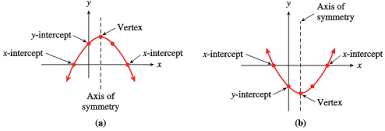
\includegraphics{parabola_graph.png}
}
\subsection{Parabolic Transformations}
\thm{Parabolic Transformations}{
    Parabola Transformations:
    \newline 
    if $a < 0$ the parabola is concave down
    \newline
    if $a > 0$ the parabola is concave up
    \newline
    if $c < 0$  move parabola down y axis
    \newline
    if $c > 0$  move parabola up y axis
    \newline
    if $b < 0$  move parabola left along x axis
    \newline
    if $b > 0$ the move parabola right along the x-axis
}
\section{Functions and their notation}
\thm{Functions and their notation}{
Functions are another way of writing equations for graphs, $y = x^{2}$ can be written as $f(x) = x^{2}$
\newline
Any set of ordered pairs is called a relation when referring to a function, a relation where each x value produces only one y value is called a function.
\newline
Any relation that also passes the vertical line test can be referred to as a Function.
\newline
The set of permissible x values in a relation is referred to as the domain
\newline
The range is the set of y coordinates the function can output into a relation
\begin{center}
    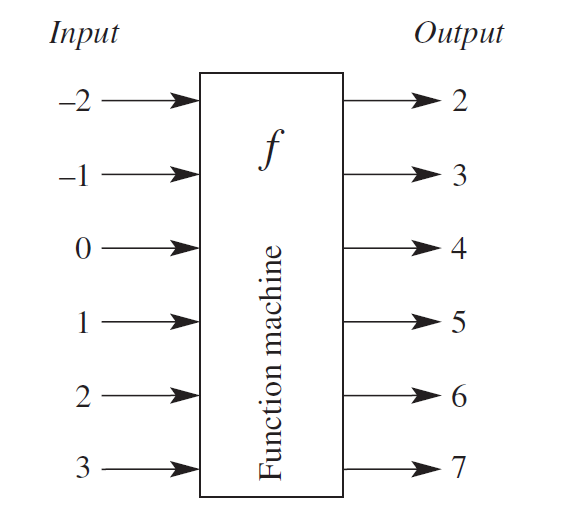
\includegraphics[scale=0.5]{functiongraphic.png}
\end{center}
}
\qs{}{\begin{center}$f(x) = 3x + 4$ find $f(\frac{1}{2})$ \end{center}}
$$f(\frac{1}{2}) = 3(\frac{1}{2}) + 4$$
$$= \frac{3}{2} + 4$$
$$= \frac{11}{2}$$
\qs{}{\begin{center} Find the domain of the following equation $f(x) = \frac{2}{x}$ \end{center}}
\begin{center}
    The domain for the equation is $x \neq 0$
\end{center}
\newpage
\section{Linear Relationships}
\subsection{Straight lines}
\subsubsection{Straight line formula}
\thm{Straight line formula}{
    Gradient states the slope of a line abbreviated to m in equations
    To find the gradient the equation is $\frac{y2-y1}{x2-x1}$
    \newline
    If the gradient is positive the  slope is uphill
    If the gradient is negative the slope is downhill
    No gradient = horizontal line
    Vertical line = Undefined line
\newline
    The straight line equation is $y = mx + c$
 where  m  is the  gradient and c  is the y-intercept
\newline


 
}
\raggedright
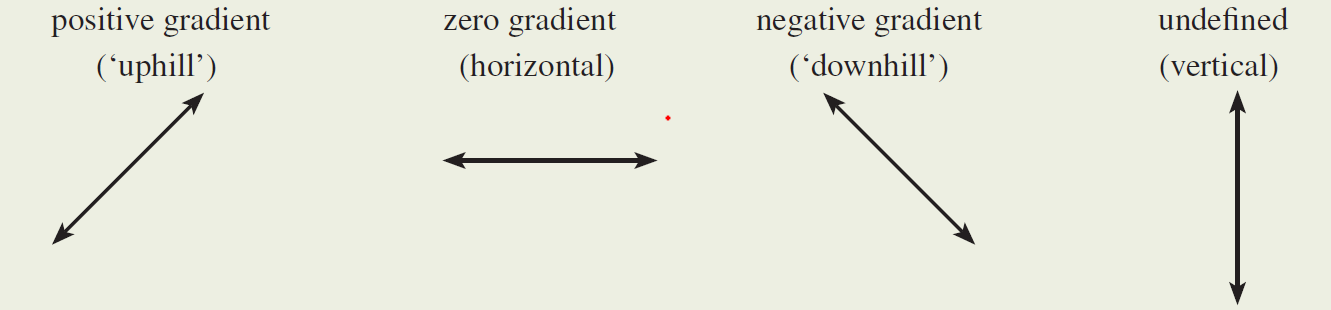
\includegraphics[scale=0.5]{gradient_lines.png}
\qs{Find Y intercept}{$$y = 2x - 8$$}
$$y = 2 \times 0 -8$$
$$ y = -8$$
\newline
\qs{Find equation of the line using the points below}{$$(3,11) (6,7)$$}
$$\frac{11-7}{3-6}$$
$$-\frac{4}{3}$$
$$y = -\frac{4}{3}x + c$$
$$11 = -\frac{4}{3} \times 3 + c$$
$$11 = 4 + c $$
$$c = 7$$
\newpage
\subsubsection{Point Gradient Formula}
\thm{Point Gradient Formula}{
    If you are given one point and  gradient you can use $y-y1 = m(x-x1)$
    where (y1, x1,) are the points on the line and m is the gradient

}
\qs{Find the equation of the line }{$$(3,2) and m = 4$$}
$$y-2 = 4(x-3)$$
$$y-2 = 4x-12$$
$$y = 4x -10$$
\qs{Find the equation of the line}{$$(-3,-4) m = -1$$}
$$y + 4 = -1(x+3)$$
$$y + 4 = -x - 3$$
$$y = -x -7$$
\subsubsection{Additional formulas} 
\thm{Additional formulas}{
    Midpoint Formula:
    \newline
    The midpoint is  between two points of a line segment, the formula is
    $M= (\frac{x1+x2}{2},\frac{y1+y2}{2})$
    \newline
    Line Segment Length:
    \newline
    The length of a line segment is the distance between two points, the formula is 
    $d = \sqrt{(x2-x1)^{2}+ (y2 - y1)^{2}}$
}
\qs{Find the midpoint}{$$(-3,-5) and (2,8)$$}
$$M = (\frac{-3 + 2}{2}, \frac{8-5}{2})$$
$$ M =(-\frac{1}{2},\frac{3}{2})$$

\qs{Find the distance between the points}{$$(-3,8) and (4, -1)$$}
$$d = \sqrt{(4+3)^{2}+(-1-8)^{2}}$$
$$d = \sqrt{7^{2}+ 9^{2}}$$
$$d = \sqrt{130}$$
\subsubsection{Parallel and perpendicular lines}
\thm{Parallel and Perpendicular lines}{
    Parallel Lines:
    \newline
    All parallel lines have the same gradient
    \newline
    Perpendicular lines:
    \newline
    To find perpendicular lines $ m1 \times m2 = -1$ or $ m2 = -\frac{1}{m1}$, m2 is the negative reciprocal of m1

}
\qs{Are these lines perpendicular or parallel}{$$ y = \frac{1}{2}x + 2$$ \centering and $$ 2y - x = 5$$}
$$2y = x + 5$$
$$ y = \frac{1}{2}x + \frac{5}{2}$$
$$These lines are parallel to each other$$
\qs{Are these lines perpendicular or parallel}{$$ y = -3x-8$$ \centering and $$y = \frac{1}{3}x+ 1$$}
$$ -3 \times \frac{1}{3} = -1$$
$$Thes lines are perpendicular$$
\newpage
\subsection{Simultaneous Equations}
\subsubsection{Simultaneous Equations Substitution}
\thm{Simultaneous Equations Substitution}{
    The substitution method is used to solve simultaneous equations when one pronumeral is isolated and can be substituted into the other equation
}
\qs{}{$$1.2x-3y = -8$$ $$2.y = x + 3$$}
\centering Sub 2 into 1
$$2x -3(x + 3) = -8$$
$$2x -3x -9 = -8$$
$$x = -1$$
$$ y = -1 + 3$$
$$y = 2$$
$$(-1,2)$$
\begin{note}
 Always remember to isolate pronumerals before substituting
\end{note}
\qs{}{$$1.y = -3x + 2$$  $$2.y = 7x -8$$}
\centering Sub 1 into 2
$$ 7x - 8 = -3x + 2$$
$$10x = 10$$
$$ x =  1$$
$$y = 7 -8$$
$$ y = -1$$
$$(1,-1)$$
\newpage
\raggedright
\subsubsection{Simultaneous Equations Elimination}
\thm{Simultaneous Equations Elimination}{
    The elimination method is used when you cannot isolate one variable and the equation is in the form of $ax + by = d$
    \newline
    The method used to complete the elimination method is multiplying both equations by a chosen factor and then adding or subtracting one of the equations from the other to eliminate a variable
}
\qs{}{$$1.x + y = 6$$ \centering $$2.3x - y = 10$$}
\centering add 1 to 2
2a.$$4x = 16$$
$$x = 4$$
$$4 + y = 6$$
$$ y = 2$$
\begin{note}
    Once you find one variable, sub into an equation to find the other
\end{note}

\qs{}{$$1.3x + 2y = 6$$ \centering and $$2.5x + 3y = 11$$}
\centering 1. times 3
\centering 2. times 2
$$1a. 9x + 6y = 18$$
$$2a. 10x + 6y = 22$$
\centering 2a - 1a
$$ x = 4$$
$$12 + 2y = 6$$
$$ y = -3$$
\begin{note}
    When multiplying the equations by the chosen factor, remember that  one coefficient and variable in each equation should be the same
\end{note}
\newpage
\raggedright
\subsection{Linear Inequalities}
\thm{Linear inequalities }{
    We solve Linear inequalities the same way we solve linear equations except we flip the sign if we multiply or divide by a negative.
    \newline
    When drawing linear inequalities we use an open circle if the greater or less than signs are used, We use a closed circle if the greater/less than or equal to symbols are used.
}
\qs{}{$$3x + 4 > 13$$}
$$3x > 9$$
$$ x > 3$$
\qs{}{$$4 -\frac{x}{3} \leq 6$$}
$$-\frac{x}{3} \leq 2$$
$$x \geq -6$$
\section{Indices and Surds}
\subsection{Surds}
\subsection{Surd Rules and Simplification }
\thm{Surds Rules and Simplification }{
    Surds are irrational numbers that don't have a terminating decimal, surds use $ \sqrt{}$ 
    \newline
    Surd Rules:
    \newline
    $\sqrt{x^{2}} = x$
    \newline
    $\sqrt{xy} = \sqrt{x} \times \sqrt{y}$
    \newline
    $\sqrt{\frac{x}{y}} = \frac{\sqrt{x}}{\sqrt{y}}$
    \newline 
    When a factor of a number is a perfect square, its called a square factor
    \newline 
    Simplifying Surds:
    \newline
    To simplify a surd look for square factors of that number $\sqrt{50} = \sqrt{25 \times 2} = 5\sqrt{2}$
}
\qs{Simplify the following Surd}{$$\sqrt{32}$$}
$$ \sqrt{16 \times 2}$$
$$4\sqrt{2}$$
\qs{Simplify the following Surd}{$$\sqrt{\frac{75}{9}} $$}
$$\frac{\sqrt{25 \times 3}}{3}$$
$$\frac{5\sqrt{3}}{3}$$
\subsubsection{Adding and Subtracting Surds}
\thm{Adding and Subtracting Surds}{
    Like surds are multiples of the same surd, only like surds can be added or subtracted. 
    \newline
    Remember to simplify surds before adding or subtracting them
}
\qs{}{$$2\sqrt{3}+ 4\sqrt{3}$$}
$$=6\sqrt{3}$$
\qs{}{$$5\sqrt{2} - \sqrt{8}$$}
$$=5\sqrt{2} - \sqrt{4 \times 2} $$
$$=5\sqrt{2} - 2\sqrt{ \times 2} $$
$$3\sqrt{2}$$

\subsubsection{Multiplying and Dividing Surds}
\thm{Multiplying and Dividing}{
    When multiply surds use $a\sqrt{x} \times b\sqrt{y} = ab\sqrt{xy}$
    \newline
    When dividing surds use $\frac{a\sqrt{x}}{b\sqrt{y}} = \frac{a}{b} \sqrt{\frac{x}{y}}$
    \newline 
    Also, remember to use the distributive law to expand brackets
}
\qs{}{$$2\sqrt{3} \times 3\sqrt{15}$$}
$$6 \sqrt{45}$$
$$6 \sqrt{9 \times 5}$$
$$18 \sqrt{5}$$
\begin{note}
    Remember to times all square numbers by the number multiply the surd as seen above
\end{note}
\qs{}{$$\frac{12\sqrt{18}}{3 \sqrt{3}}$$}
$$\frac{12}{3}\sqrt{\frac{18}{3}}$$
$$4\sqrt{6}$$
\begin{note}
    Always separate the fraction before simplifying when dividing Surds
\end{note}
\subsubsection{Rationalising the Denominator}
\thm{Rationalising the denominator}{
    Rationalising the denominator involves multiplying the entire fraction 
    by the surd, denominator to rationalise it to a whole number
}
\qs{}{$$\frac{2\sqrt{6}}{5\sqrt{2}}$$}
$$\frac{2\sqrt{6}}{5\sqrt{2}} \times \frac{\sqrt{2}}{\sqrt{2}}$$
$$\frac{2\sqrt{12}}{10}$$
$$\frac{4\sqrt{3}}{10}$$
$$\frac{2\sqrt{3}}{5}$$
\qs{}{$$\frac{1-\sqrt{3}}{\sqrt{3}}$$}
$$\frac{1-\sqrt{3}}{\sqrt{3}} \times \frac{\sqrt{3}}{\sqrt{3}}$$
$$\frac{\sqrt{3}-3}{3}$$
\newpage

\subsection{Indices}
\subsubsection{Fractional Indices}
\thm{Fractional Indices}{
    $a^{\frac{1}{n}} = \sqrt[n]{a}$
    this is the nth root of a
    \newline
    $a^{\frac{m}{n}}  = (\sqrt[n]{a})^{m}$
}
\qs{Write in index form}{$$\sqrt[4]{x^{7}}$$}
$$=x^{\frac{7}{4}}$$
\qs{Write in surd form}{$$5^{\frac{2}{3}}$$}
$$= \sqrt[3]{5^{2}}$$
\subsubsection{Exponential Equations}
\thm{Exponential Equations}{
    An exponential equation looks like $a^{x} = b$, there is only one 
    solution to an exponential equation like the above. Many of these equations can be solved by  using 
    the same base for each exponent
}

\qs{}{$$25^{x}= 125$$}
$$(5^{2})^{x} = 5^{3}$$
$$2x = 3$$
$$x = \frac{3}{2}$$

\qs{}{$$3^{2x-1}= 27^{x}$$}
$$3^{2x-1}= 3^{3x}$$
$$2x-1= 3x$$
$$x = -1$$
\newpage
\section{Statistics}
\subsection{Types of Statistics and Data Displays}
\thm{Types of Statistics and Data Displays}{
    Types of Statistics:
    \newline
    There are two types of Statistics Categorical and Numerical, within these types there are subsections or statistics.
    \newline
    For Categorical Data there are nominal and Ordinal data. Nominal data has no order ie red, green blue. Ordinal data can be ordered ie low medium high.
    \newline
    For Numerical, there are Discrete and Continuous data. Discrete data can only have a limited amount of values ie the number of children in a family. For Continuous Data, it can take any value of numbers in a range ie time taken to run a race.
    \newline
    Types of Data sets:
    \newline
    There are three types of data sets, Symmetrical where the mean and median will be equal, 
    \newline
    Positively Skewed where the median will be less than the mean and
   \newline
    Negatively skewed where the median will be greater than the mean.
    See the Figures Above for a visual representation


}
\begin{figure}
    \centering
    \begin{subfigure}[b]{0.3\textwidth}
        \centering
        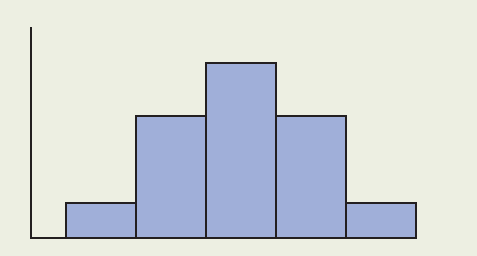
\includegraphics[width=\textwidth]{symmetrical_data.png}
        \caption{The median and mean will be equal}
        \label{Symmetrical Data}
    \end{subfigure}
    \hfill
    \begin{subfigure}[b]{0.3\textwidth}
        \centering
        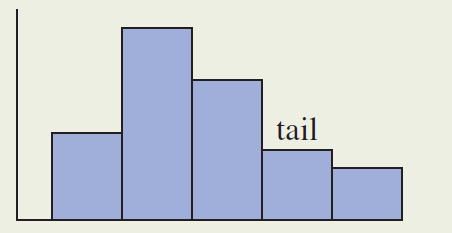
\includegraphics[width=\textwidth]{positive_data.png}
        \caption{The median will be less than the mean}
        \label{Positively skewed Data}
    \end{subfigure}
    \hfill
    \begin{subfigure}[b]{0.3\textwidth}
        \centering
        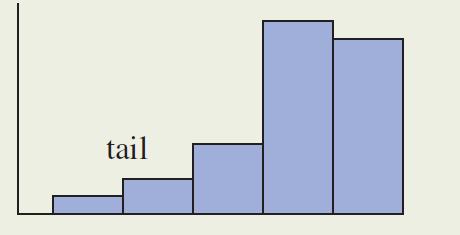
\includegraphics[width=\textwidth]{negative_data.png}
        \caption{The median will be greater than the mean}
        \label{Negatively Skewed Data}
    \end{subfigure}
       \caption{SYMMETRICAL AND SKEWED DATA}
       \label{fig:three graphs}
\end{figure}
\subsection{Summary Statistics}
\thm{Summary Statistics}{
    Summary statistics highlight important aspects of a data set
    \newline
    The median is the middle value of a data set, when the data set is even you should divide the middle two numbers by 2
    \newline
    The mode is the most frequently occurring value in a dataset
    \newline
    \newline
    The frequency and the percentage frequency are the number of times a 
    favourable outcome occurred. To get percentage frequency you 
    divide the number of favourable outcomes by the total outcomes.
    \newline
    \newline
    Five-figure summary:
    \newline
    Min/max value, the smallest/largest value in a dataset
    \newline
    Lower Quartile($Q_1$), the value above $25\%$ of the ordered data. The formula to obtain $Q_1$ is $ 0.25(n+1)$ with n being the number of data points given.
    \newline
    \newline
    The median($Q_2$), the value above $50\%$ of the ordered data.
    \newline
    \newline
    Upper Quartile($Q_3$), the value above $75\%$ of the ordered data. The formula to obtain $Q_1$ is $ 0.25(n+1)$ with n being the number of data points given.
    \newline
    \newline
    \newline
    A measure of spread:
    \newline
    Range = max value - min value
    \newline
    Interquartile Range(IQR). The formula for this is $Q_3 Q_1$
    \newline
    Standard deviation(SD)
    Outliers are outside the parameters o a data set, to detect if a data point is an outlier the formula is  $ if <  Q_1 - 1.5 \times IQR $ or $ > Q_3 + 1.5 \times IQR$
}
\subsection{Box Plots}
\thm{Box Plots}{
    Box Plots are used to summarise data sets, the dataset is divided into four groups as seen in the figure below,
    \begin{center}
        \includegraphics[scale=0.5]{boxplot.png} 
    \end{center}
    An outlier is marked with an x on the plot
}
\subsection{BiVariate Data}
\thm{Bivariate Data}{
    Types of correlation with bivariate data:
    \begin{center}
        \includegraphics[scale=0.3]{correlation.png}
    \end{center}

}
\subsection{Line of Best fit}
\thm{Line of best fit}{
What is a line of best fit?
\newline
A line of best fit is placed on a graph with an even amount of points across each side, this shows the trend of the data.
\newline
To find the line of best fit you can use the straight line formula or Point gradient Formula.
\newline
This line can be used for extrapolation or interpolation 
}
\section{Probability}
\subsection{Arrays}
\thm{Arrays}{
An array is used to list the data of a two-step experiment.
If replacement is allowed in the experiment then the outcome can occur in both steps of the experiment
However, if replacement is not allowed. the outcome cannot occur in both steps of the experiment, w highlight these possibilities with an X in the array table
}
\subsection{Tree Diagrams}
\thm{Tree Diagrams}{
Tree diagrams are used to list the probability of outcomes in an experiment with two or more steps
\newline
The branches on the tree describe the probability of an outcome at each stage. To gain the probability of an outcome occurring you multiply the probability of each branch by each other.
See the diagram below for example:
}

\includegraphics[scale=0.25]{treediagram.png}
\section{Measurement}
\subsection{Area of quadrilaterals }
\thm{Area of quadrilaterals}{
Area formulas:
\newline
Rhombus : $ \frac{1}{2}xy$
\newline
Parallelogram: $bh$
\newline 
Trapezium: $ h\left(\frac{a+b}{2}\right)$
\newline
Kite: $\frac{1}{2}xy$
}
\subsection{Cylinders and Prisms}
\subsubsection{SA  of Cylinders and Prisms}
\thm{SA of Cylinders and Prisms}{
    To find the Surface area of  objects you need to find the area of each 2d shape that make up the 3d object
    \newline
    To find the SA of a cylinder the formula is $2\pi$$r^{2}+ \pi$$dh$ with (d) being the diameter and (h) being the height
    \newline
    To find the SA of a prism the formula is $ 2(w \times h) + 2(h \times l) + 2(l \times w)$
}
\qs{}{If the radius of a cylinder is 3 and the height of the cylinder is 3 what is the SA, leave your answer in exact form}
$$SA = 2\pi3^{2} + \pi6 \times 3$$

$$=18\pi + 18\pi$$
$$=36\pi$$
\qs{}{If the height of a prism is 5 and the length of the prism is 7 and the width of a prism is 2 find the SA}
$$SA = 2(2 \times 5) + 2(7 \times 5) + 2(2 \times 7) $$
$$= 40 + 70 + 28$$
$$=138$$
\newpage
\subsubsection{Volume of Cylinders and Prisms}
\thm{Volume of Cylinders and Prisms}{
To calculate the volume of a cylinder and prism you first need to find the area of the cross-section that makes up that shape.
The volume formula for a cylinder is $ \pi$$r^{2} \times h$
\newline
The volume formula for a prism is $ah$ where a is the area of the cross-section of the shape.
}
\qs{}{Find the volume of a prism where the width is 2m, length is 3m and height is 4 m}
$$V = 4(2 \times 3)$$
$$= 24$$

\qs{}{Find the volume of a cylinder where the radius is 2m and the height is 6m in exact form}
$$V = \pi2^{2} \times 6$$
$$ = 24\pi$$
\newpage
\subsection{Pyramids and cones}
\subsubsection{SA of Pyramids and Cones}
\thm{SA of Pyramids and Cones}{
    The formula for the surface area of a right cone is $\pi$$rl + \pi$$r^{2}$ where l is the slant height, if you need to find the slant height or any measurement in a  cone use the Pythagorean theorem, the Sine rule or Cosine Rule
    \newline
    The surface area for a right pyramid is $4(b \times h) + b^{2}$
}
\qs{}{The slant height of a cone is 4 and the radius of a cone is 6, what is the SA in exact form}
$$SA = \pi6 \times 7 + \pi6^{2}$$
$$= 42\pi + 36\pi$$
$$ = 78\pi$$
\qs{}{ The base of a pyramid is 4 and the height is 6 find the SA}
$$SA = 2(4 \times 6) + 4^{2}$$
$$= 48 + 16$$
$$= 64$$
\subsubsection{Volume of Pyramids and Cones}
\thm{Volume of Pyramids and Cones}{
To find the volume of a right pyramid or cone the formula $\frac{1}{3}AH$ where A is the area of the pyramids or cone cross-section, $x^{2}$ for pyramid  or$\pi$$r^{2}$ for cone.
 
}
\qs{}{Find the volume of this pyramid if the length is 4 and the height is 6}
$$V = \frac{1}{3}4^{2} \times 6$$
$$=\frac{16}{3} \times 6$$
$$=\frac{96}{3}$$
$$=32$$
\newpage
\qs{}{Find the volume of a cone in the exact form if the radius is 10 and the height is 15}
$$V =\frac{1}{3}(\pi10^{2}) \times 15$$
$$=\frac{100\pi}{3} \times 15$$
$$=\frac{1500\pi}{3}$$
$$=500\pi$$
\subsection{Spheres}
\subsubsection{SA of Spheres}
\thm{SA of Spheres}{
The formula for a Spheres SA is $4\pi$$r^{2}$
}
\qs{}{If the radius of the sphere is 3 find the SA in exact form}
$$SA = 4\pi3^{2}$$
$$=4\pi9$$
$$=36\pi$$
\qs{}{If the radius of a sphere is 5 find the SA in exact form}
$$SA=4\pi5^{2}$$
$$=100\pi$$
\subsubsection{Volume of a Sphere}
\thm{Volume of a Sphere}{
The formula for the Volume of a Sphere is $\frac{4}{3}\pi$$r^{3}$
}
\qs{}{If the Radius of the sphere is 7 find the volume in exact form}
$$\frac{4}{3}\pi7^{3}$$
$$\frac{4}{3}343\pi$$
$$\frac{1372\pi}{3}$$
\qs{}{If the radius of a sphere is 3 find the volume in exact form}
$$\frac{4}{3}\pi2^{3}$$
$$\frac{4}{3}8\pi$$
$$\frac{32\pi}{3}$$
\section{Trigonometry}
\subsection{Trigonometric Ratios}
\thm{Trigonometric Ratios}{
Trigonometric ratios help us find the angles inside a RAT
\newline
The three trigonometric Ratios:
\newline
$Sin\theta = \frac{opp}{hyp}$
\newline
$Cos\theta = \frac{adj}{hyp}$
\newline
$Tan\theta = \frac{opp}{adj}$
\newline
A mnemonic to remember these ratios is SOHCAHTOA
\newline
To find the unknown length of a side you can find a ratio that links the angle and the two sides together  and solve for $x$ See the second example below
\newline



}
\qs{}{Find the angle if the adjacent side is 5 and the hypotenuse 7 }
$$\cos\theta = \cos^{-1} \frac{5}{7}$$
$$\cos\theta = 44.4$$
\qs{}{Find the unknown side if the opp is 5cm, hyp = unknown and the angle is 50 }
$$\sin50 = \frac{5}{x}$$
$$x = \frac{5}{\sin50}$$
$$x = 6.53$$
\begin{note}
    Remember  if the variable is the numerator multiply the ratio and the length, if the variable is the denominator remember to divide the length by the variable
\end{note}
\subsection{Bearings}
\thm{Bearings \textbf{Come back to this later}}{
Bearings are three-digit numbers that give us a more accurate direction
}
\qs{}{}
\qs{}{}
\subsection{Obtuse Angles and Unit Circle}
\thm{Obtuse angles and Unit Circle}{
The unit circle has a radius of 1. It is used to define the values of $Cos\theta$ $Sin\theta$ and $Tan\theta$
\newline
Obtuse Angles:
\newline
To find the angle supplementary to an obtuse angle in the Q2 use the below 
\newline
$cos(180 - \theta)=  -cos\theta$
\newline
$sin(180 - \theta)= sin\theta$
\newline
$tan(180 - \theta)= -tan\theta$
\newline
A mnemonic to remember the sign in each of the four Quadrants is All Stations To Central(ALL SIN TAN COS) in the first quadrant(acute) all values are positive and in the Second only Sin is positive. etc.
\newline
\newline
Exact Values for the trigonometric Ratios can be obtained using two triangles seen below
\includegraphics[scale=0.5]{exactvaluetriangles.png}
\newline
Here are the values in a table:
\begin{center}
\includegraphics[scale=0.5]{exactvalues.png}
\end{center}
}
\newpage
\qs{}{Find the supplementary angle that goes with $\sin150$}
$$\theta=\sin180-150$$
$$=30$$
$$\sin30=\frac{1}{2}$$
\qs{}{Find the supplementary angle that goes with $\tan135$}
$$\theta=\tan180-135$$
$$= \tan45$$
$$\tan45 = 1$$

\subsection{Sine Rule}
\thm{The Sine Rule}{
 The Sine rule describes the relationship between the angles in a triangle and their opposite sides, being that they're equal.
 \newline
 the Sine Rule is $\frac{a}{\sin(A)} = \frac{b}{\sin(B)} = \frac{c}{\sin(C)}$, this rule can be manipulated to find either the side length or angle size.
 \newline
 It is important to note that to use the sine rule you need to know the size of one angle, the length of the side opposite that angle, and another side or angle.
\begin{center}
    \includegraphics[scale=0.5]{sinediagram.png}   
\end{center}
}
\newpage
\qs{}{Find for x in the following: \begin{center}\includegraphics[scale=0.5]{qs1.png}\end{center}}
$$\frac{x}{\sin39}= \frac{22}{\sin57}$$
$$x = \frac{22 \times \sin39}{\sin57}$$
$$x = 16.51cm$$
\qs{}{Find $\theta$ in the following: \begin{center} \includegraphics[scale=0.5]{qs2.png} \end{center}}
$$\frac{\sin\theta}{20}= \frac{\sin78}{28}$$
$$\sin\theta = \frac{20 \times \sin78}{28}$$
$$\sin\theta = 44.32$$
\begin{note}
    Remember to use $\sin^{-1}($ to gain the size of the angle. Additionally when using the sine rule to find  an angle, use the reciprocal of the rule stated in the theorem 
\end{note}
\newpage
\subsection{Cosine Rule}
\thm{Cosine Rule}{
    The cosine rule describes the relationship between three sides and one angle in a triangle.
    \newline
    The rule to find a side is $a^{2} = b^{2} + c^{2} - 2bc\times \cos(A)$
    \newline
    The rule to find the angle is $\cos(A) = \frac{b^{2} + c^{2} - a^{2}}{2bc}$
    \newline
    You can use the Cosine Rule when you are given two sides and angles and you are required to find the third side. You are required to find the angle when given three sides
    \newline
    Checking your answer, the longest side is opposite the largest $\angle  \therefore$ smallest angle is opp smallest $\angle$
}
\qs{}{Solve for the missing side \begin{center} \includegraphics[scale=0.5]{qs3.png}\end{center}}
$$a^{2} = 7^{2} + 11^{2} -2\times 7 \times 11 \times \cos(125) $$
$$a = \sqrt{258.33}$$
$$a = 16.07cm$$
\qs{}{Solve for $\theta$ \begin{center} \includegraphics[scale=0.5]{qs4.png}\end{center}}
$$\cos\theta = \frac{5^{2}+7^{2}- 8^{2}}{2 \times 5 \times 7}$$
$$= \frac{10}{70}$$
$$= \cos^{-1}\left(\frac{1}{7}\right)$$
$$\theta=81.79$$
\newpage
\subsection{Area Rule}
\thm{Area Rule}{
The area rule is primarily used for NRATS but you can use it for RATS as well, it relates two sides of a triangle plus the including angle with the area.
\newline
The formula is $A = \frac{1}{2}ab\sin(C)$
}
\qs{}{Find the area \begin{center} \includegraphics[scale=0.5]{qs5.png}\end{center}}
$$A = \frac{1}{2}\times 3 \times 5 \times \sin(36)$$
$$A= 4.41cm^{2}$$
\qs{}{Solve for x \begin{center} \includegraphics[scale=0.5]{qs6.png}\end{center}}
$$22 = \frac{1}{2}\times 12 \times x \times \sin(40) $$
$$\frac{22}{6\sin(40)} = x$$
$$x = 5.7mm^{2}$$
\subsection{The four Quadrants}
\thm{The four Quadrants}{
   Dependent on the quadrant the angle is, the angle ratio could be positive or negative:
   \newline
   Q1(0-90): All ratios are positive
   \newline
   Q2(90-180): Only Sine Ratio is positive
    $180 - \theta$
    \newline
   Q3(180-270): Only the Tan ratio is positive, to get this angle the equation is $\theta - 180$
   \newline
   Q4(270-360): Only the Cosine ratio is positive the equation to find the cute angle is $360 - \theta$
   \newline
   A mnemonic to remember this is All Stations to Central
}
\qs{}{Find the acute angle if it is 280}

$$\theta = 360 - 280$$
$$\theta = 80 = -tan(80), -sin(80), cos(80)$$
\
\newpage
\subsection{Trigonometric Function Graphs}
\thm{Trigonometric exact value graphs}{
    Here are the graphs that show the pattern of trigonometric exact values
    \newline
    Sine Wave:
    \begin{center}
    \includegraphics[scale=0.5]{sinewave.png}
    \newline
    \end{center}
    Cosine Wave:
    \begin{center}
    \includegraphics[scale=0.3]{coswave.png}
    \newline
    \end{center}
    Tangent Wave:
    \begin{center}
    \includegraphics[scale=0.7]{tanwave.png}
    \end{center}

}
\section{Geometry}
\subsection{Triangle Congruency}
\thm{Triangle Congruency}{
Two triangles are considered to be congruent when they are the same shape and size

Triangle congruency can be proven using one of the tests below:
\newline
\newline 
SSS(3 Sides): The three sides of each triangle are equal to each other
\newline
SAS(Two sides one angle):  The two sides and the including angle of the triangles are equal to each other
\newline
AAS( Two angles and one side ): The two angles and one side of the triangles are equal
\newline
RHS(right-angle, hypotenuse, side): One side, 90-degree angle and the hypotenuse of triangles are equal 
}
\qs{}{Prove this pair of triangles is congruent \begin{center} \includegraphics[scale=0.5]{qs7.png} \end{center}}
$$BC = EF (given)$$
$$AB = DE (given)$$
$$\angle ABC = \angle DEF (given)$$
$$\therefore \triangle ABC = \triangle DEF (SAS)$$
\qs{}{Prove this pair of triangles is congruent \begin{center} \includegraphics[scale=0.5]{QS8.png} \end{center}}
$$EF = CB (given)$$
$$\angle EDF = \angle CAB (given)$$
$$\angle EFD = \angle ACB (given)$$
$$\therefore \triangle EDF = \triangle CAB (AAS)$$
\newpage 
\subsection{Similarity in shapes\textbf{ADD QUESTIONS}}

\thm{Similarity in Shapes}{
For two figures to be considered similar, they need to be the same shape(proportional) but have different 
sizes.
\newline
The symbol used to describe similarity in shapes is
\newline
To prove two shapes are similar we can use four different tests:
\newline
PPP(three proportional sides): Three sides of each triangle are proportional to each other
\newline
PAP(two proportional sides and included angle): Two sides of each triangle are proportional and the included angle is equal
\newline
AA(Two Angles): Two angles in each triangle are equal to each other
\newline
RHS(right angle, hypotenuse, side): The right angle, hypotenuse and side are proportional to each triangle

}
\qs{}{Prove these two triangles are similiar \begin{center} \includegraphics[scale=0.5]{qs9.png} \end{center}}
$$\angle DCE = \angle ACB (vert opp)$$
$$\angle CDE = \angle ABC (alt angles)$$
$$\therefore \triangle DCE ||| \triangle ACB (AA)$$

\qs{}{Prove these two triangles are similar \begin{center} \includegraphics[scale=0.5]{qs10.png} \end{center}}
$$\angle BAC  = \angle EDF (given)$$
$$\angle ABC  = \angle DEF $$
$$\therefore \triangle BAC ||| \triangle EDF (AA)$$
\subsection{Circle terminology and chord properties}
\begin{figure}
    \centering
    \begin{subfigure}[b]{0.3\textwidth}
        \centering
        \includegraphics[width=\textwidth]{chord.png}
        \caption{The Chord is a segment whose both points lie on a circular arc}
        \label{Chord}
    \end{subfigure}
    \hfill
    \begin{subfigure}[b]{0.3\textwidth}
        \centering
        \includegraphics[width=\textwidth]{arc.png}
        \caption{An arc is a smooth curve joining two endpoints}
        \label{ARC}
    \end{subfigure}
    \hfill
    \begin{subfigure}[b]{0.3\textwidth}
        \centering
        \includegraphics[width=\textwidth]{segment.png}
        \caption{A segment is part of the circle which is cut off by a chord or secant}
        \label{Segment}
    \end{subfigure}
       \caption{STypes of lines in Circles}
       \label{fig:three circles}
\end{figure}
\thm{Circle terminology and Chord properties}{
Look at the figures above to revise basic circle terms, an important term to remember is subtended which is a mathematical term for make/made.
\newline
An angle is subtended by an arc/chord when the arms of the angle arms meet the chord/arc's endpoint. See the example below.
\newline
\begin{center}
\includegraphics[scale=0.3]{chordangle.png}
\end{center}
Rules about Chords:
\newline
\noindent\begin{minipage}{0.3\textwidth}% adapt widths of mini pages to your needs
    \includegraphics[width=\linewidth]{chordequal.png}
    \end{minipage}%
    \hfill%
    \begin{minipage}{0.6\textwidth}\raggedright
    Chords of equal length subtend equal angles at the centre of a circle, and chords that subtend equal angles are equal length.
    \end{minipage}

\noindent\begin{minipage}{0.3\textwidth}% adapt widths of minipages to your needs
    \includegraphics[width=\linewidth]{chordcentre.png}
\end{minipage}%
        \hfill%
\begin{minipage}{0.6\textwidth}\raggedright
        Chords which are equal distances from the centre are equal, and chords of equal length are equal distances from the centre.
\end{minipage}

\noindent\begin{minipage}{0.3\textwidth}% adapt widths of minipages to your needs
    \includegraphics[width=\linewidth]{chordperp.png}
\end{minipage}%
        \hfill%
\begin{minipage}{0.6\textwidth}\raggedright
    The perpendicular from the centre of a circle bisects the chord, and a line through the centre of a circle that bisects a chord
    is perpendicular to the chord.
\end{minipage}
\noindent\begin{minipage}{0.3\textwidth}% adapt widths of mini pages to your needs
    \includegraphics[width=\linewidth]{chordbisect.png}
\end{minipage}%
        \hfill%
\begin{minipage}{0.6\textwidth}\raggedright
Perpendicular bisectors of each chord intersect at the centre of a circle, you can use two perp bisectors to find the circle centre.
\end{minipage}

}


\qs{}{Given AB = CD and OE = 3 cm , find OF.\begin{center} \includegraphics[scale=0.5]{qs11.png} \end{center}}
\ centre {$OF = 3cm$ (chords of equal length are the same distance from centre)}
\qs{}{Given $OM \perp AB$, AB = 10 cm and $\angle AOB = 92$ ,  find AM and $\angle AOM$ \begin{center} \includegraphics[scale=0.5]{qs12.png} \end{center}}
\center{$AM = 5cm$, perp centre bisects chord}
\begin{center}
    $\angle AOM = 92\div 2 = 46$
\end{center}
\raggedright
\subsection{Circle Angle properties}
\thm{Circle angle properties}{
     Here are the angle properties at the centre and circumference of a circle
     \newline
     The angle at the circumference of a circle is $\frac{1}{2}$ the size of the angle at the centre when standing on the same arc. The angle at the circumference is called an inscribed angle. See diagram.
     \begin{center}
        \includegraphics[scale=0.5]{circleangleprop.png}
     \end{center}
     The inscribed angle theory states that Angles subtended by the same arc are equal. See diagram.
     \begin{center}
        \includegraphics[scale=0.5]{inscribedangle.png}
     \end{center}
     The angle formed by the diameter to a point on a semi-circle is 90
     \begin{center}
        \includegraphics[scale=0.5]{diameterangle.png}
     \end{center}
     Opposite angles in a cyclic quadrilateral add to 180 degrees, as long as all vertices touch the circumference of the Circle. See diagram.
     \begin{center}
        \includegraphics[scale=0.5]{cyclicquadangle.png}
     \end{center}
}
\qs{}{Find the value of $a$\begin{center}\includegraphics[scale=0.5]{QS13.png}\end{center}}
\begin{center}
    $a = 30$ inscribed angles on the same arc are equal
 \end{center}
 \qs{}{Find the value of $x$\begin{center}\includegraphics[scale=0.5]{qs14.png}\end{center}}
 \begin{center}
     $x = 80$ centre angles are 2 times the size of an inscribed angle when standing on the same arc
  \end{center}

\subsection{Tangent Theorems}
\thm{Tangent Theorems}{
    What is a tangent? A tangent is a line that has one point of contact with the circle/object.
    \newline
    In a circle, the tangent intersects the circle once and the tangent is perpendicular to the radius at the point of contact.
    \newline
    Two tangents that originate at the same point are equal.
    \newline
    Alternate angle theorem:
    \newline
    The angle formed between the tangent and the chord through the point of contact of the tangent is equal to the angle formed by the chord in the alternate segment. See diagram.
    \begin{center}
        \includegraphics[scale=0.5]{alternateangletheorem.png}
     \end{center}
}
\qs{}{Solve for $a$     \begin{center}
    \includegraphics[scale=0.5]{qs15.png}
 \end{center}}
 \begin{center}
    $\angle BOA = 90$ alternate angle theorem
\end{center}
    $$180 -(90 + 71) = 19$$
    $$\therefore \angle OBA = 19$$
    \qs{}{Solve for $a$     \begin{center}
        \includegraphics[scale=0.3]{qs16.png}
     \end{center}}
$$\angle BOA = 360-243 = 117$$
\begin{center}
$\angle OBP = \angle OAP = 90$ alternate angle theorem
\end{center}
$$a = 360- (117 + 90 + 90) = 63$$
$$a = 63$$
\section{Logarithms and Polynomials}
\subsection{Logarithm Intro}
\thm{Logarithm Intro}{
    Logarithms are is used to find the power a base was raised to get a value.
    \newline
    Example:
    \newline
    $\log_2(16)= 4$ since$   2^{4} = 16$
    \newline
    The way a log is written is the base is the subscript, and the value of the equation is inside the function which outputs the exponent ie $a^{x} = y$ $=\log_a(y) = x$
}
\qs{}{\centering Write $10^{2} = 100$ in log form}
$$\log_{10}(100) = 2$$
\qs{}{
\centering Write $\log_{7}(49) = 2$ in index form}
$$7^{2} = 49$$
\subsection{Log Laws}
\thm{Log Laws}{
    The Log laws Relate to index Laws, the log laws help us simplify and expand Logs  when needed
    \newline

    Product Rule:
    \newline
    $log_{a}(xy) = log_{a}(x) + log_{a}(y)$ This law relates to the  index law of $ a^{x}\times a^{y} = a^{x+y}$
    \newline
    Quotient Rule:
    \newline
    $\log_{a}(\frac{x}{y}) = \log_a{x} - log_{a}{y}$ This relates to $a^{m}\div a^{n} = a^{m-n}$
    \newline
    Power Rule:
    \newline
    $\log_{a}(x^{n}) = n\log_a{x}$ This law relates to $(a^{m})^{n}= a^{m\times n}$
    \newline
    Change of Base Rule:
    \newline
    $\log_{a}(x) = \frac{\log_{b}(x)}{\log_{b}(a)}$
    \newline
    $\log_a{\frac{1}{x}} = \log_{a}(x^{-1}) = -\log_{a}(x)$
}
\qs{}{Simplify$$\log_{a}(3)+ \log_{a}(2)$$}
$$\log_{a}(6)$$
\qs{}{Simplify$$2\log_{a}(3)$$}
$$\log_{a}(3^{2})$$
\end{document}